%% ----------------------------------------------------------------
%% Thesis.tex -- MAIN FILE (the one that you compile with LaTeX)
%% ---------------------------------------------------------------- 

% Set up the document
\documentclass[a4paper, 11pt, oneside]{Thesis}  % Use the "Thesis" style, based on the ECS Thesis style by Steve Gunn
\graphicspath{{../svnit_thesis_final/Figures/}}  % Location of the graphics files (set up for graphics to be in PDF format)

% Include any extra LaTeX packages required
\usepackage[square, numbers, comma, sort&compress]{natbib}  % Use the "Natbib" style for the references in the Bibliography
\usepackage{verbatim}  % Needed for the "comment" environment to make LaTeX comments
\usepackage{vector}  % Allows "\bvec{}" and "\buvec{}" for "blackboard" style bold vectors in maths
\usepackage[section]{placeins}
\usepackage{amsmath,amssymb,amsopn,amstext,amsfonts}
%\graphicspath{{../figures/}}
\hypersetup{urlcolor=blue, colorlinks=true}  % Colours hyperlinks in blue, but this can be distracting if there are many links.

%% ----------------------------------------------------------------
\begin{document}
	\frontmatter      % Begin Roman style (i, ii, iii, iv...) page numbering
	
	% Set up the Title Page
	\title  {Low Cost Drone Development System for Precision Farming}
	\authors  {\texorpdfstring
		{{\textbf{MOSAM DABHI (U13EC022)}}}
		{Mosam}\\		
		{{\textbf{MURLI PRAJAPATI (U13EC035)}}}\\
		{{\textbf{SIDDHANT LOYA (U13EC036)}}}\\		
		{{\textbf{SHIKHAR OMAR (U13EC037)}}}\\
		{{\textbf{RAJ MIGLANI (U13EC103)}}}\\
	}

	%\authors  {\texorpdfstring
%	$	{{Mosam Sanjay Dabhi}}
%		{Mosam Sanjay Dabhi}
%	}
%	\addresses  {\groupname\\\deptname\\\univname}  % Do not change this here, instead these must be set in the "Thesis.cls" file, please look through it instead
%	\date       {\today}
%	\subject    {}
%	\keywords   {}
	
	\maketitle
	%% ----------------------------------------------------------------
	
	\setstretch{1.3}  % It is better to have smaller font and larger line spacing than the other way round
	
	% Define the page headers using the FancyHdr package and set up for one-sided printing
	\fancyhead{}  % Clears all page headers and footers
	\rhead{\thepage}  % Sets the right side header to show the page number
	\lhead{}  % Clears the left side page header
	
	\pagestyle{fancy}  % Finally, use the "fancy" page style to implement the FancyHdr headers
	
	%% ----------------------------------------------------------------
	% Declaration Page required for the Thesis, your institution may give you a different text to place here
	%\Declaration{
		
	%	\addtocontents{toc}{\vspace{1em}}  % Add a gap in the Contents, for aesthetics
		
	%	I, Mosam Sanjay Dabhi, declare that this thesis titled, `Study of Efficient Mixed-Integer Planning for Autonomous Vehicles in Densely Cluttered Environments' and the work presented in it are my own. I confirm that:
		
	%	\begin{itemize} 
					
			%\item[\tiny{$\blacksquare$}] Where any part of this thesis has previously been submitted for a degree or any other qualification at this University or any other institution, this has been clearly stated.
			
		%	\item[\tiny{$\blacksquare$}] Where I have consulted the published work of others, this is always clearly attributed.
			
		%	\item[\tiny{$\blacksquare$}] Where I have quoted from the work of others, the source is always given. With the exception of such quotations, this thesis is entirely my own work.
			
		%	\item[\tiny{$\blacksquare$}] I have acknowledged all main sources of help.
			
			%\item[\tiny{$\blacksquare$}] Where the thesis is based on work done by myself %jointly with others, I have made clear exactly what was done by others and what I have contributed myself.
			%\\
		%\end{itemize}
		
		
		%Signed:\\
		%\rule[1em]{25em}{0.5pt}  % This prints a line for the signature
		
		%Date:\\
		%\rule[1em]{25em}{0.5pt}  % This prints a line to write the date
	%}
	%\clearpage  % Declaration ended, now start a new page
	
	%% ----------------------------------------------------------------
	% The "Funny Quote Page"
	\pagestyle{empty}  % No headers or footers for the following pages
	
%	\null\vfill
	% Now comes the "Funny Quote", written in italics
%	\textit{``When Larry and Sergey founded Google Search, one of the things that struck me is that it was available for everyone to use. We deeply desire our services to work for everyone. And that inherently means we have to work with partners. That is the thesis underlying everything we do.''}
	
%	\begin{flushright}
%		Sundar Pichai
%	\end{flushright}
	
%	\vfill\vfill\vfill\vfill\vfill\vfill\null
%	\clearpage  % Funny Quote page ended, start a new page
	%% ----------------------------------------------------------------
	
	% The Abstract Page
	\addtotoc{Abstract}  % Add the "Abstract" page entry to the Contents
	\abstract{
		\addtocontents{toc}{\vspace{1em}}  % Add a gap in the Contents, for aesthetics
		
Precision farming is a farming concept aimed at improving the yield of a farm by observing, measuring and analysing the crops. This aims at utilizing the latest development in the fields of UAVs, image processing, cloud and machine learning to deliver data driven plating advice. High yield of each crop is dependent on the seed, the soil, the cropping pattern, the weather, water and the use of fertilizer and the lack of pets. Considering all these parameters, hyperspectral imaging of thee crops taken by the drone helps to predict what is growing healthy and what not.

The project includes designing an autonomous Hex-copter with a Go-pro HD camera mounted using the gimbal for collecting the data of hyperspectral images. The processing of this hyperspectral image data is performed on the server by utilizing various open-source computer vision and GIS libraries. This pre-processed data is classified with the help of vegetation indices combined with machine learning algorithms. Once the critical areas of the farm are known from the above approach, a deep learning model is used to analyse the images of the crops in those critical areas to provide a prescription of the disease on a simple to use Graphical User Interface (GUI). 
		
	}
	
	\clearpage  % Abstract ended, start a new page
	%% ----------------------------------------------------------------
	
	\setstretch{1.3}  % Reset the line-spacing to 1.3 for body text (if it has changed)
	
	% The Acknowledgements page, for thanking everyone
	\acknowledgements{
		\addtocontents{toc}{\vspace{1em}}  % Add a gap in the Contents, for aesthetics
		
		We acknowledge OUR guide and advisor for this project, Dr. A. D. Darji, Assistant Professor, Electronics and Communication Engineering Department, S.V.N.I.T. for his valuable inputs and suggestions without which this report would not have been possible. 
		
		We also acknowledge 6omvi team for giving us the opprtunity for perfoming the experiments and obtain the required results.
		
	}
	\clearpage  % End of the Acknowledgements
	%% ----------------------------------------------------------------
	
	\pagestyle{fancy}  %The page style headers have been "empty" all this time, now use the "fancy" headers as defined before to bring them back
	
	
	%% ----------------------------------------------------------------
	%\lhead{\emph{Contents}}  % Set the left side page header to "Contents"
	\tableofcontents  % Write out the Table of Contents
	
	%% ----------------------------------------------------------------
	%\lhead{\emph{List of Figures}}  % Set the left side page header to "List if Figures"
	\listoffigures  % Write out the List of Figures
	
	%% ----------------------------------------------------------------
	%\lhead{\emph{List of Tables}}  % Set the left side page header to "List of Tables"
	\listoftables  % Write out the List of Tables
	
	%% ----------------------------------------------------------------
	\setstretch{1.5}  % Set the line spacing to 1.5, this makes the following tables easier to read
	\clearpage  % Start a new page
	%\lhead{\emph{Abbreviations}}  % Set the left side page header to "Abbreviations"
	%\listofsymbols{ll}  % Include a list of Abbreviations (a table of two columns)
	%{
	% \textbf{Acronym} & \textbf{W}hat (it) \textbf{S}tands \textbf{F}or \\
	%\textbf{LAH} & \textbf{L}ist \textbf{A}bbreviations \textbf{H}ere \\
	
	%}
	
	%% ----------------------------------------------------------------
	\clearpage  % Start a new page
	%\lhead{\emph{Physical Constants}}  % Set the left side page header to "Physical Constants"
	%\listofconstants{lrcl}  % Include a list of Physical Constants (a four column table)
	%{
	% Constant Name & Symbol & = & Constant Value (with units) \\
	%Speed of Light & $c$ & $=$ & $2.997\ 924\ 58\times10^{8}\ \mbox{ms}^{-\mbox{s}}$ (exact)\\
	
	%}
	
	%% ----------------------------------------------------------------
	
	%\lhead{\emph{Symbols}}  % Set the left side page header to "Symbols"
	%\listofnomenclature{lll}  % Include a list of Symbols (a three column table)
	%{
	% symbol & name & unit \\
	%$a$ & distance & m \\
	%$P$ & power & W (Js$^{-1}$) \\
	%& & \\ % Gap to separate the Roman symbols from the Greek
	%$\omega$ & angular frequency & rads$^{-1}$ \\
	%}
	%% ----------------------------------------------------------------
	% End of the pre-able, contents and lists of things
	% Begin the Dedication page
	
	\setstretch{1.5}  % Return the line spacing back to 1.3
	
	\pagestyle{empty}  % Page style needs to be empty for this page
	%\dedicatory{For/Dedicated to/To my\ldots}
	
	\addtocontents{toc}{\vspace{2em}}  % Add a gap in the Contents, for aesthetics
	
	
	%% ----------------------------------------------------------------
	\mainmatter	  % Begin normal, numeric (1,2,3...) page numbering
	\pagestyle{fancy}  % Return the page headers back to the "fancy" style
	
	% Include the chapters of the thesis, as separate files
	% Just uncomment the lines as you write the chapters
	
	\chapter{Introduction}

Agricultural production system is an outcome of a complex interaction of seed, soil, water and agro-chemicals (including fertilizers). Therefore, judicious management of all the inputs is essential for the sustainability of such a complex system. The focus on enhancing the productivity during the Green Revolution coupled with total disregard of proper management of inputs and without considering the ecological impacts, has resulted into environmental degradation. The only alternative left to enhance productivity in a sustainable manner from the limited natural resources at the disposal, without any adverse consequences, is by maximizing the resource input use efficiency. It is also certain that even in developing countries, availability of labour for agricultural activities is going to be in short supply in future. The time has now arrived to exploit all the modern tools available by bringing information technology and agricultural science together for improved economic and environmentally sustainable crop production. Precision agriculture merges the new technologies borne of the information age with a mature agricultural industry. It is an integrated crop management system that attempts to match the kind and amount of inputs with the actual crop needs for small areas within a farm field. This goal is not new, but new technologies now available allow the concept of precision agriculture to be realized in a practical production setting.

Many technological developments occurred in the last decade that has improvised the concept of Precision Farming (PF). Precision agriculture (PA) or satellite farming or site specific crop management (SSCM) is a farming management concept based on observing, measuring and responding to inter and intra-field variability in crops.~\cite{mcbratney2005future,whelan2003definition} The goal of precision agriculture research is to define a decision support system (DSS) for whole farm management with the goal of optimizing returns on inputs while preserving resources. The adaptability of this technique relies on the integration and utilisation of modern days technologies such new advance farm technologies with the single system site specific technologies. The technology varies from high speed connectivity of internet, farmer awareness. PF is an integrated, information and agricultural management system that is designed to improve the whole farm production efficiency with the low cost effect while avoiding the unwanted effects of chemical loading to the environment. The focus under PF is to gather information regarding the soil and crop condition and capture the sequence on the soil and crop conditions at spatial level.

\section{Motivation}

Precision agriculture means application of precise and correct amount of inputs like water, fertilizer, pesticides etc. at the correct time to the crop for increasing its productivity and maximizing its yields. Precision agriculture management practices can significantly reduce the amount of nutrient and other crop inputs used while boosting yields. Farmers thus obtain a return on their investment by saving on phytosanitary and fertilizer costs. The second, larger scale benefit of targeting inputs in spatial, temporal and quantitative terms concerns environmental impacts. Applying the right amount of inputs in the right place and at the right time benefits crops, soils and groundwater, and thus the entire crop cycle. Consequently, precision agriculture has become a cornerstone of sustainable agriculture, since it respects crops, soils and farmers. Sustainable agriculture seeks to assure a continued supply of food within the ecological, economic and social limits required to sustain production in the long term. Precision agriculture therefore seeks to use high-tech systems in pursuit of this goal. 

In a developing country like India the use of precision farming can help to boost the economic growth in agriculture via substantial increase in crop yield. The overall cost and infrastructure needed to meet this goal still seems a challenging task to be accomplished. We therefore decided to build an end-to-end solution for precision farming by building a low cost system. 

\section{System Overview}
We aim to design a low cost system to solve the problems discussed above and help the farmers gain better insights of the farms. A flowchart of the system is shown in Fig.~\ref{fig: extra-1}. The system consists of image capturing of the farm by the drone. These images are then uploaded on the server for image processing and analysis. The analyzed image is  overlaid on Google Maps for better visualization of the farm showing critical areas in different colors. The photographs of the critical areas can be uploaded on our applictaion to be evaluated for prescription of crop diseases.
\begin{figure}[!h]
	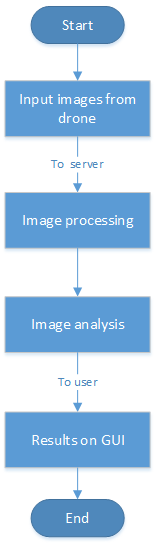
\includegraphics[height=0.9\linewidth]{extra-1}
	\centering
	\caption{\label{fig: extra-1}Flowchart of the System Workflow}
\end{figure}.


\section{Objectives}

The main objectives of the project are:

\begin{itemize}
	\item Build a low cost drone with the use of a flight controller having the functionality of stable and autonomous flight. (having capability of hovering and following the flight of guided waypoints)
	\item Perform image processing to stitch the images using Open Drone Map
	\item Perform image analysis with two approaches i.e. Vegetation 	Index(VI) methods and machine learning on hyperspectral data, and deep learning on RGB data.
	\item Build a Graphical User Interface(GUI) and an Android Application.
\end{itemize}


\section{Structure of the document}
The report is divided into five chapters with each part describing different aspects of the project. The second chapter presents a literature survey on the knowledge obtained on the topic. The third chapter describes the methods and tools used to build/assemble the drone required for above mentioned functionality. The fourth chapter provides insights into the image processing techniques applied to achieve the best results. The fifth chapter describes the methods used for image analysis. The sixth chapter deals with the development of the GUI for the end user clients.


 % Introduction
	
	\chapter{Literature Survey}

Non-stop supply of nutritious food production for the ever increasing population as well because the challenges of global market have factored in the need for newer efficient farming systems. Precision Farming is a scientific approach to enhance the agricultural management by adoption of data to spot, analyse and manage the spatial and temporal viability of science parameters. 


Most conservation researchers and practitioners currently rely on satellite-based remote sensing for mapping and monitoring land use change~\cite{broich2011time}. However, remote sensing technology might not be accessible for many developing-country researchers due to financial constraints. Although certain low-resolution satellite images are freely available (e.g., Landsat~\cite{LandsatS1:online} and MODIS ~\cite{LandsatS40:online}), other sub-meter resolution images can be prohibitively costly (e.g., QuickBird ~\cite{LandsatS4:online}, IKONOS ~\cite{geoeyeco87:online}). Yet, such high-resolution data are often critical for accurately detecting and tracking land use change at the landscape scale.

Furthermore, much of the humid tropics is often obscured from remote sensing satellites due to a persistent cloud cover~\cite{hansen2008method}. As such, cloud-free satellite images for a specific time period and location are often not readily available. Researchers typically have to search from a time series of images to obtain the cloud-free data they require, thus rendering any real-time monitoring of land-use change practically impossible. 

\section{Drone Development and operation}
The autopilot system of such precision farming drones is based on the ‘ArduPilot Mega’ (APM), which has been developed by an online community of ``diydrones''~\cite{diydrone38:online}. The APM includes a computer processor, geographic positioning system (GPS), data logger, pressure and temperature sensor, airspeed sensor, triple-axis gyro, and accelerometer. By combining the APM with an open-source mission planner software (APM Planner), most remote control model airplanes could be con verted to an autonomous drone~\cite{ardupilo77:online}.

Previous versions of APM 2.6 had only the onboard compass which resulted in very large offsets during the flight tests and even in calibration phase. Due to off-board compass amalgamated with GPS, accuracy of the autonomous flight is considerably increased. Also, proper tuning was not available easily in the previous versions.

Our choice of flight controller is also based on which type of rotor we would be using.  As we are using Multi Rotor and not a fixed wing machine, APM 2.5 doesn't seem to catch up with the applicative need of our mission of multi-rotor(hex-copter). If we are flying a fixed-wing rotor (plane) then APM 2.5 is the better choice as its slightly cheaper and due to the space we can mount the APM away from magnetic interference (motors/ESC). Also the higher speed Mediatek module is better suited to faster moving vehicles. While if we are flying Multi-rotor (hex-copter), then its best to go with the APM 2.6 as the GPS module is better suited to slower moving platforms, and the external compass allows us to mount it away from interferance from all the ESC's we have on Multicopters~\cite{APM25orA25:online}.



\section{Spectral signature of vegetation}

A plant leaf does not absorb all wavelengths uniformly since it consists of biochemical and chemical substances with different absorption peaks. It is documented that various pigments - such as chlorophyll-a and chlorophyll-b,  anthocyanin, $\alpha$ and $\beta$-carotenoids, lutein, violaxanthin - the physical structure of leaves and their water content are the main factors determining the spectral signature ~\cite{zwiggelaar1998review,campbell2011introduction}.

An interesting point is that these components change during the season, depending on the phenophase, species, and nutrient conditions. The spectral signatures of leaves can therefore be utilized to monitor various plant conditions, such as nutrient and water deficiency, and to identify crop types and weeds. 

At the canopy level, the absorption peaks of the chemical substances generally become unclear, since reflectance from canopy is strongly influenced by leaf size, plant density, number of layers, orientation of leaves, and other environmental factors such as soil reflectance and light angle~\cite{campbell2011introduction}. However, some of the biochemical properties are still detectable from the canopy reflectance. Indeed, the canopy reflectance spectrum has been used to identify crop types~\cite{serpico1996experimental} and weeds~\cite{goel2002use,goel2003potential,lamb1999evaluating,lass1996detection}, to detect water and nutrient stress~\cite{goel2002use,goel2003potential,lelong1998hyperspectral,shibayama1993canopy}, and to estimate crop phenology~\cite{railyan1993red,boissard1993reflectance}, leaf area index~\cite{aparicio2002relationship,rastogi2000estimation,shibayama1989seasonal} and plant biomass~\cite{serrano2000remote}.

\section{Image Stitching}
In the stitching method mentioned in~\cite{chen2014image} first of all feature extraction takes place through harris corner detection and feature is matched by finding the normalized cross correlation between them. After that ransac is used to remove the outliers and to eliminate the error matching. Another method overcome the limitation of SIFT i.e. sensitive to non linear illumination changes~\cite{yang2014image}. In this method initially feature points are extracted by SYFM(a local symmetry based descriptor)and SIFT(gradient based descriptor). Then SIFT descriptor and local symmetry are combined to characterize those feature point. After that feature matching is carried out by ``randomized kd trees'' and transform parameters are calculated by correct inner points after ransac was used to eliminate wrong matches. In the case of drone image stitching we must understand the fact that the images have GPS points encoded in them , which can be used to stitch the images . This method gives better result than other methods because apart from the features which we extract from images we can use the GPS points to arrange and stitch the images characterize those feature point. After that feature matching is carried out by ``randomized kd trees'' and transform parameters are calculated by correct inner points after ransac was used to eliminate wrong matches.

\section{Vegetation Indices and Machine Learning}
Over the years, a number of vegetation indices (VIs) have been developed by combining two or more wavebands in the hyperspectral images in ratios and/or differences, to highlight various crop conditions. However, one of the problems in applying VIs to crop yield estimation is the difficulty in choosing the most appropriate vegetation index in a specific situation~\cite{barrett1999fractional}. In fact, various environmental factors, such as background effects and crop canopy conditions, have been shown to be potential sources of noise, which affect the spectral reflectance in canopy level~\cite{aparicio2000spatial}.

Artificial intelligence and especially machine learning have contributed to the creation of control systems in agriculture. There are a lot of machine learning algorithms like Support Vector Machines(SVM), Simple Multivariate Linear Regressions(SMLR), Decision Trees(DT), Neural Networks(NN), etc. available that can be utilized for recognizing intricate patterns in data.

Applying machine learning models in addition to the VI based methods have resulted in great results as shown by Farid Melgani and Lorenzo Bruzzone in ~\cite{melgani2004classification}.


\section{Deep Learning for Image-Based Plant Disease Detection}
Crop diseases are a major threat to food security, but their rapid identification remains difficult in many parts of the world due to the lack of the necessary infrastructure.

Modern technologies have given human society the ability to produce enough food to meet the demand of more than 7 billion people. However, food security remains threatened by a number of factors including climate change[1], the decline in pollinators~\cite{bay2008speeded}, plant diseases~\cite{dalal2005histograms}, and others. Plant diseases are not only a threat to food security at the global scale, but can also have disastrous consequences for smallholder farmers whose livelihoods depend on healthy crops. In the developing world, more than 80 percent of the agricultural production is generated by smallholder farmers~\cite{deng2009imagenet}, and reports of yield loss of more than 50\% due to pests and diseases are common~\cite{ehler2006integrated}. Furthermore, the largest fraction of hungry people (50\%) live in smallholder farming households~\cite{everingham2010pascal}, making smallholder farmers a group that’s particularly vulnerable to pathogen-derived disruptions in food supply.

Various efforts have been developed to prevent crop loss due to diseases. Historical approaches of widespread application of pesticides have in the past decade increasingly been supplemented by integrated pest management (IPM) approaches~\cite{garcia2013comparison}. Independent of the approach, identifying a disease correctly when it first appears is a crucial step for efficient disease management. Historically, disease identification has been supported by agricultural extension organizations or other institutions such as local plant clinics. In more recent times, such efforts have additionally been supported by providing information for disease diagnosis online, leveraging the increasing internet penetration worldwide. Even more recently, tools based on mobile phones have proliferated, taking advantage of the historically unparalleled rapid uptake of mobile phone technology in all parts of the world~\cite{bold2012mobile}. 


Smartphones in particular offer very novel approaches to help identify diseases because of their tremendous computing power, high-resolution displays, and extensive built-in sets of accessories such as advanced HD cameras. It is widely estimated that there will be between 5 and 6 billion smartphones on the globe by 2020. At the end of 2015, already 69\% of the world’s population had access to mobile broadband coverage, and mobile broadband penetration reached 47\% in 2015, a 12-fold increase since 2007~\cite{bold2012mobile}. The combined factors of widespread smartphone penetration, HD cameras, and high performance processors in mobile devices lead to a situation where disease diagnosis based on automated image recognition, if technically feasible, can be made available at an unprecedented scale. 

Computer vision, and object recognition in particular, has made tremendous advances in the past few years. The PASCAL VOC Challenge~\cite{he2016deep}, and more recently the Large Scale Visual Recognition Challenge (ILSVRC)~\cite{hernandez2014integrating} based on the ImageNet dataset~\cite{huang2007application} have been widely used as benchmarks for numerous visualization-related problems in computer vision, including object classification. In 2012, a large, deep convolutional neural network achieved a top-5 error of 16.4\% for the classification of images into 1,000 possible categories~\cite{hughes2015open}. In the following three years, various advances in deep convolutional neural networks lowered the error rate to 3.57\% ~\cite{hughes2015open,facts2015figures,jia2014caffe,krizhevsky2012imagenet,lecun1989backpropagation}.


\section{Summary}

In the literary review, we have enlisted the various techniques that are currently being used in precision farming using Unmanned Aerial Vehicle(UAV). We based our prototype drone on a popular model airplane (DJI Model). This hex-copter is relatively inexpensive, lightweight, and has ample room within its fuselage for installing the APM and an onboard camera. The Hex-copter is also be equipped with a video camera. We used a GoPro HD Hero camera housed within a protective shockproof casing~\cite{NewTab52:online}. This camera was attached to the belly of the hex-copter and pointed at around 45 degrees forwards and downwards. Previously VI based methods have been used for image analysis. But these methods seem to be greatly affected by environmental noise. Machine learning has also shown good results in this field and therefore, a combination of VI based method and machine learning  is used for the analysis of the farm. The role of GIS in different agricultural scenarios has also been discussed. The use of deep learning for crop disease prediction is also employed for providing bettter prescription to the farmers. The model and approach for an agricultural system can be easily noted by analysis of past work. Thus such literature allows for an easy yet fast approach towards a complete prototype. % Literature Survey
	
	\chapter{Image Data Collection using Autonomous Drone}

\section{About}

This chapter deals with complete specifications of our vehicle used for the penultimate applications of using for precision farming applications. The focus of this chapter is to lay out a complete overview of our system used with the causes and outputs related to the precision farming applications. Which flight mode is to be used at what time, how would those flight modes be accessed, significance of PID Autotune, why making a dataset of farm images is necessary, etc. are some of the questions we have tried to answer in this chapter. 

During our field tests, the drone was powered by a 2200 mAh (milliampere-hour) battery, which allowed it to fly for around 25 minutes per mission, and over a total distance of approximately 15 km. Using the APM Planner (version 1.1.26), we programmed the flight path of each mission by clicking on waypoints in a Google satellite map interface. The drone can be programmed to take off and land autonomously, and circle over any waypoint for a specified number of turns or duration. We also programmed other flight parameters such as ground speed and altitude of each waypoint. Each pre-programmed mission was uploaded to the drone, which would then fly the mission autonomously.


We would be discussing the overview, selection of flight controller, detailed specification of physical parameters used by our system, sensors used for our application, flight modes representing Autotune, Loiter mode(hover) and guided waypoint ultimately resulting in an autonomous flight. We would be making the dataset of images available as open-source so that public can utilize this data for machine learning purposes. 

The overall pipeline showcasing the system flow is displayed in Fig.~\ref{fig: asda}

\begin{figure}[!h]
	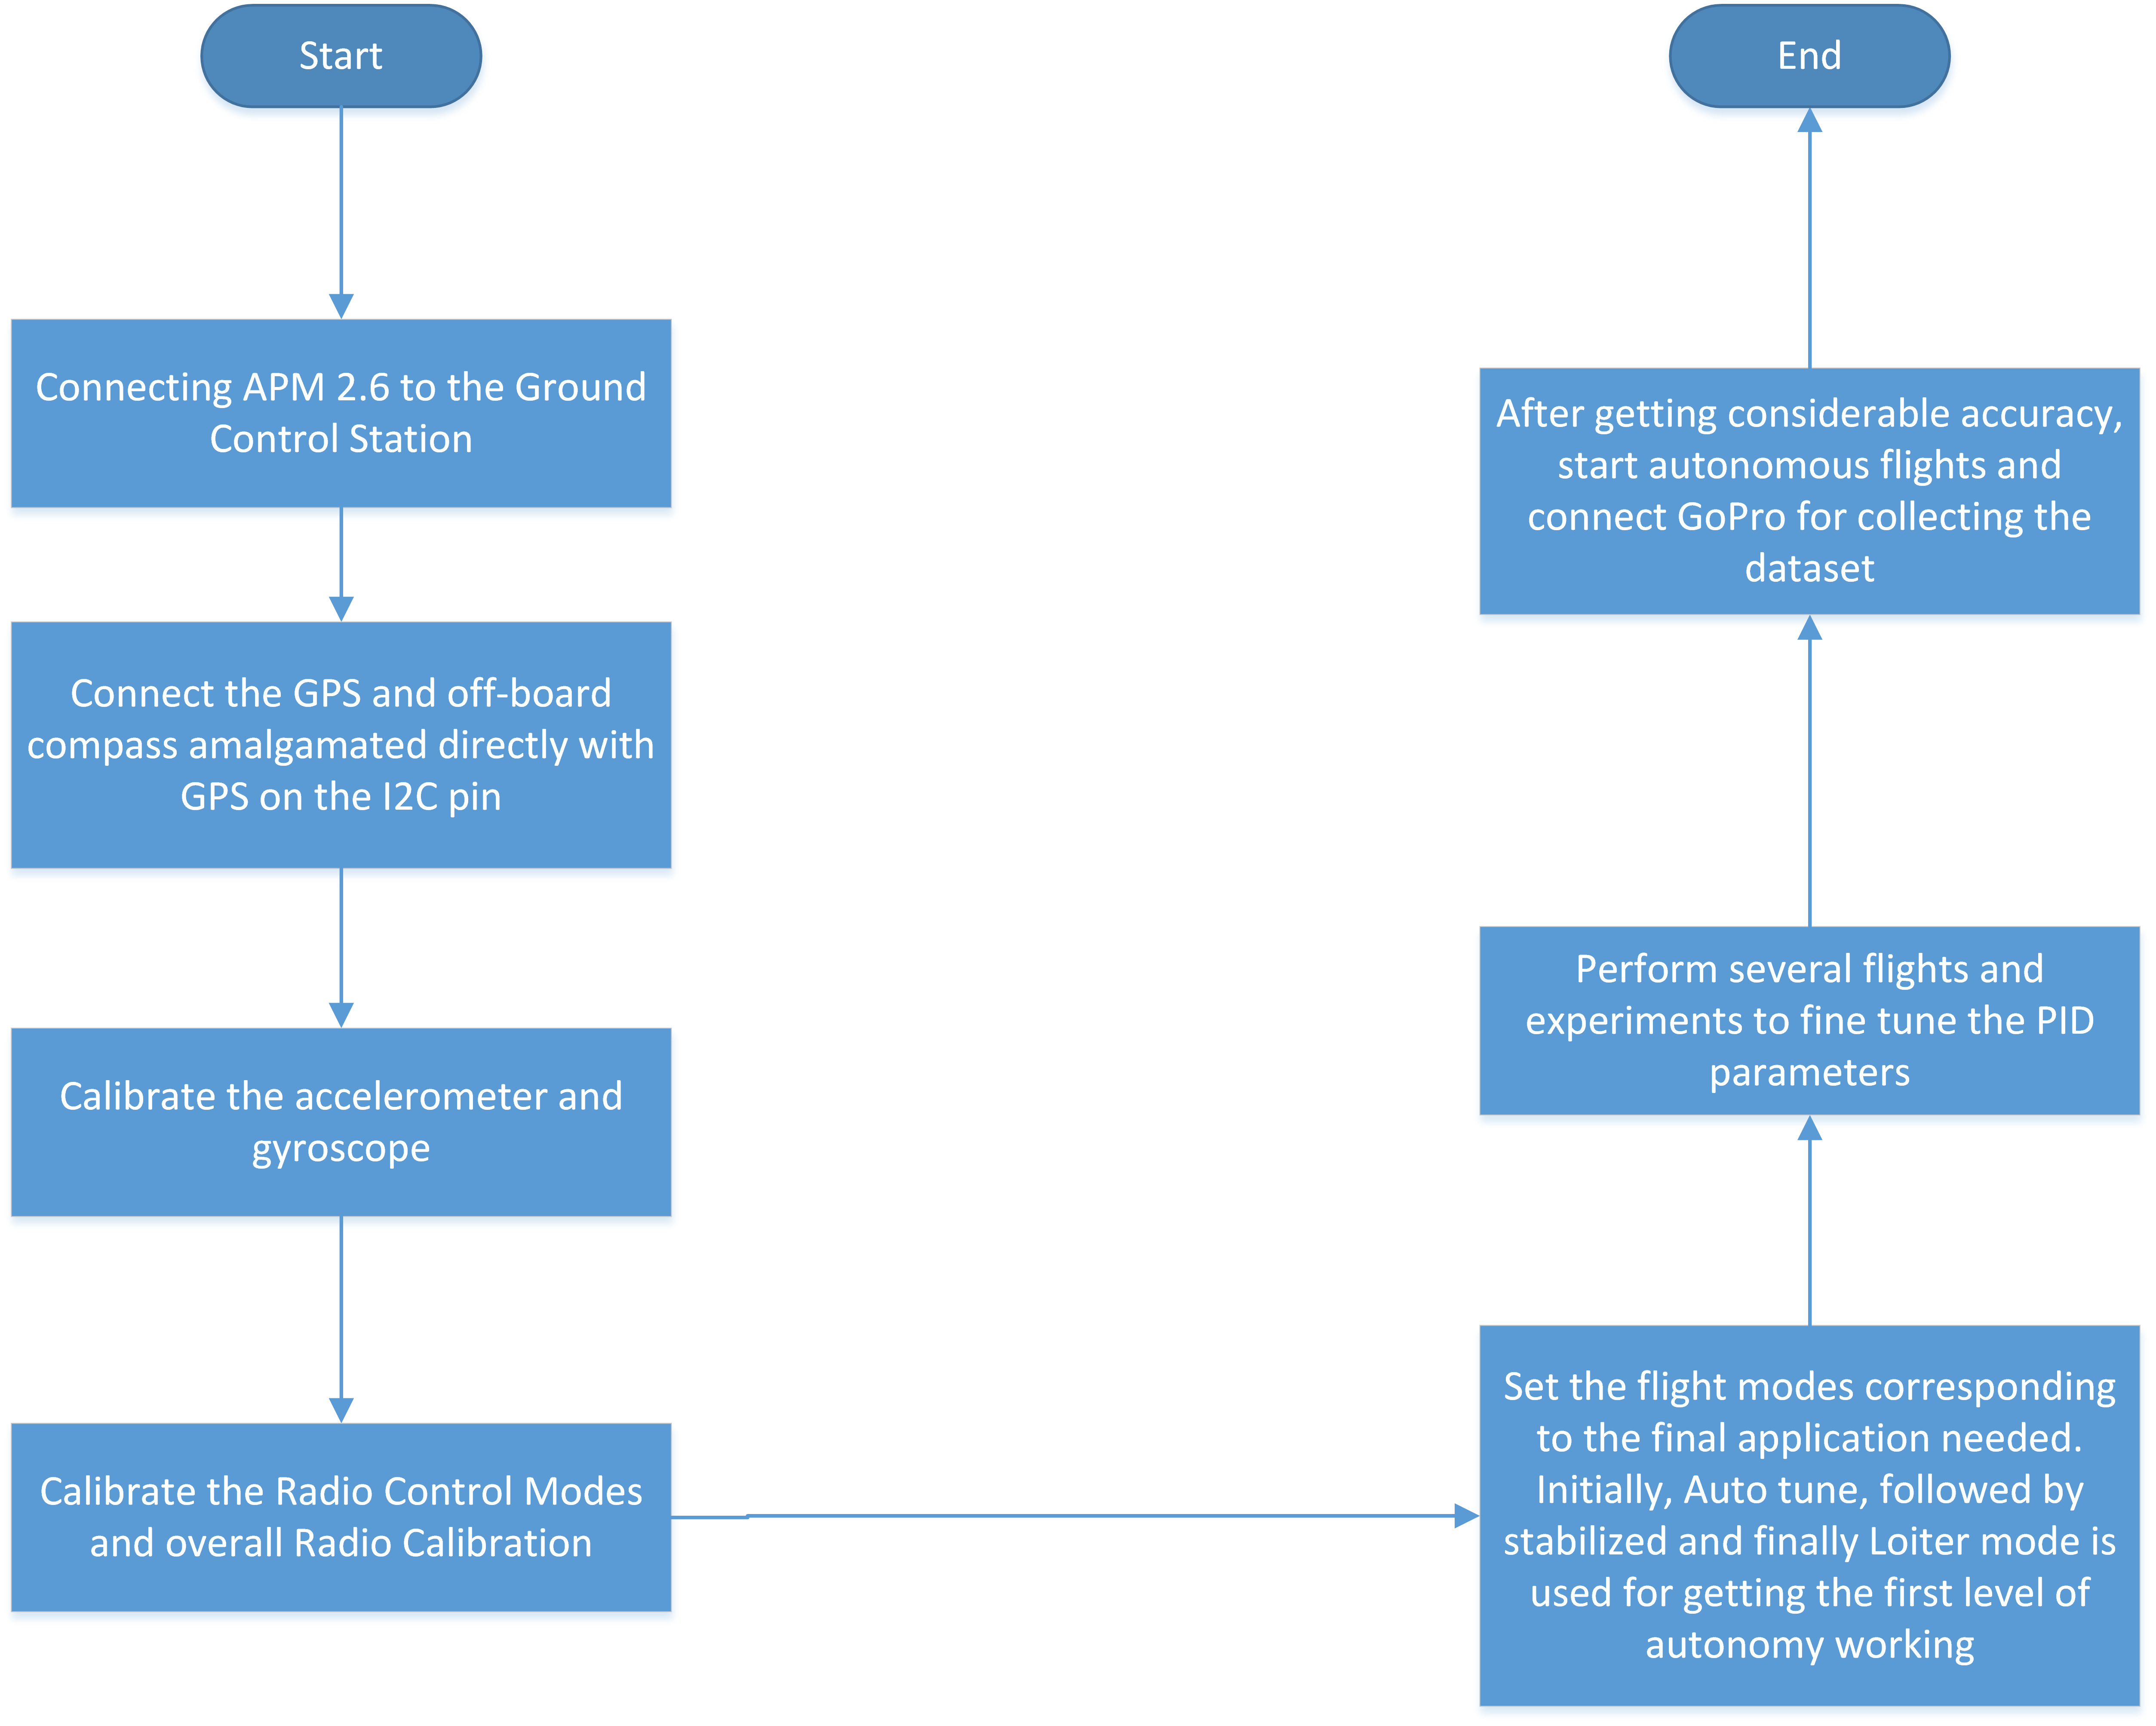
\includegraphics[width=1.0\linewidth]{asda}
	\centering
	\caption{\label{fig: asda}Pipeline of the autonomous hex-copter flight system}
\end{figure}.
A proper working sytem of the pipeline shown in Fig.~\ref{fig: asda} is accomplished and displayed in chapter ``Chapter 7 - Experimental Results''.


\section{Overview of the System}


The reason we zeroed in on using the overview flow as shown in Fig.~\ref{fig: img_1} and using APM system was because it is an open-source autopilot solution for multi-rotor vehicles, offering both enhanced remote control flight (via a number of intelligent flight modes) and execution of fully autonomous missions~\cite{19}. As part of the wider ArduPilot software platform it works seamlessly with Ground Control Station software that can monitor vehicle telemetry and perform powerful mission planning activities. It also benefits from other parts of the Ardupilot ecosystem, including simulators, log analysis tools, and higher level APIs for vehicle management and control. 

\begin{figure}[h]
	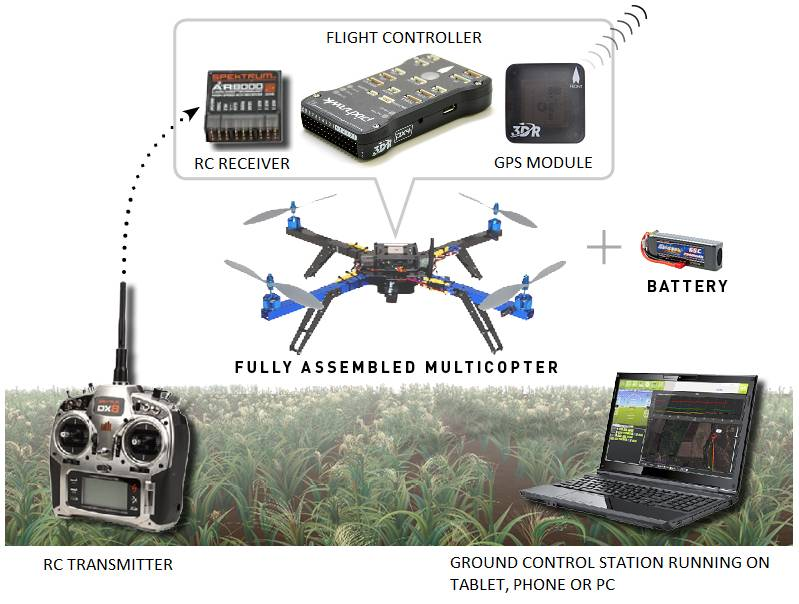
\includegraphics[width=0.9\linewidth]{img_1}
	\centering
	\caption{\label{fig: img_1}Overview of our system}
\end{figure}.

\subsection{Choosing a Flight Controller}
ArduPilot runs on many different flight controller boards. Selecting the right board depended on the physical restraints of the vehicle and the applications we wanted to run. Due to it's gracious presence and impression in open-source domain and the popularity in its forums, we retained our system to APM 2.6 Flight controller as our need for gathering data by flying upon agricultural fields either with autonomy or hand-held control was being accomplished by this system.


That being the prime reason for choosing APM 2.6 Controller as shown in Fig.~\ref{fig: 3 and 4}. Also, the APM 2.6 board requires no assembly, and is ready for firmware. We have a choice of side or top entry pin configuration, in order to accommodate a variety of installations. 

APM 2.6 is a revision of the APM that makes use of an external compass. Our APM 2.6 had no on board compass, and it is optimized for vehicles where the compass should be placed as far from power and motor sources as possible to avoid magnetic interference. Our APM 2.6 is designed to be used with the 3DR GPS uBlox LEA-6 with Compass module. We mounted the GPS/Compass module further from noise sources than the APM itself. APM 2.6 required a GPS unit with an on board compass for full autonomy, the condition fulfilled by our system.

\begin{figure}[t]
	\hfill
	\subfigure[]{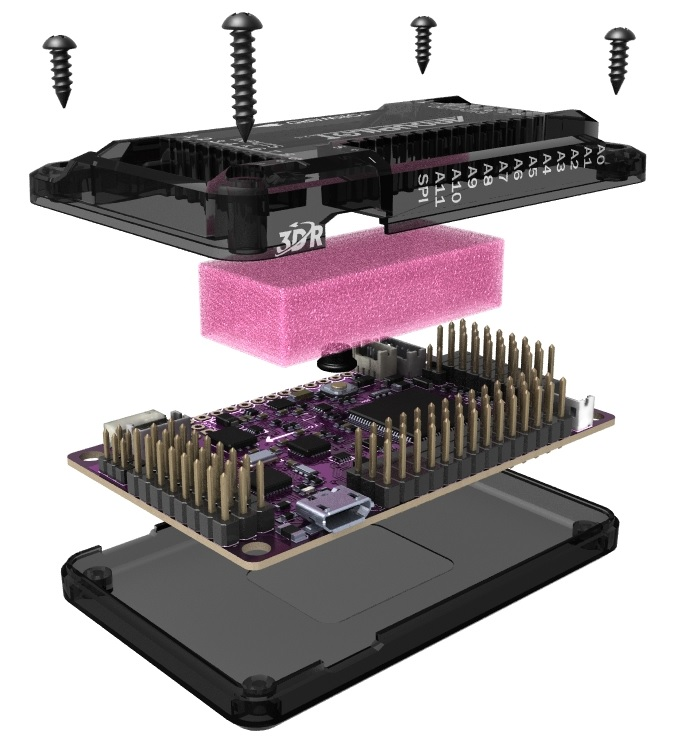
\includegraphics[width=0.48\linewidth]{3}}
	\hfill
	\subfigure[]{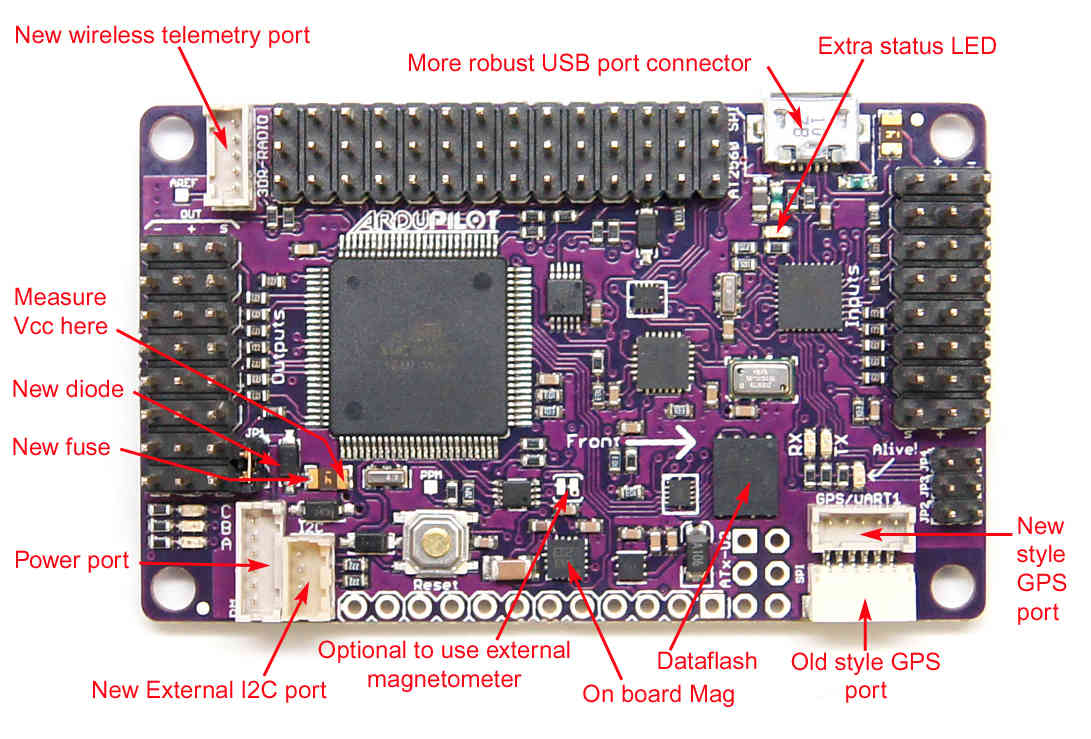
\includegraphics[width=0.48\linewidth]{4}}
	\hfill
	\caption{\label{fig: 3 and 4}APM 2.x overview~\cite{19}}
\end{figure}


\section{Physical Parameters pertaining to our system}
6 brushless DC motors of 1000kV are used on our hex-copter. Detailed specifications of Sensors, Electrical parameters and Mechanical parameters are described below.
\subsection{Sensors}
\begin{itemize}
	\item \textbf{MPU6000}: 3 accelerometers, 3 gyroscopes and 1 temperature sensor
	\item \textbf{MPU9250}: 3 accelerometers , 3 magnetometers, 3 gyroscopes and 1 temperature sensor
	\item \textbf{LSM9DS0}: 3 accelerometers , 3 magnetometers, 3 gyroscopes and 1 temperature sensor
	\item \textbf{MS5611-01BA}: 1 digital pressure sensor (barometer) and 1 temperature sensor
\end{itemize}

\subsection{Electrical}

\begin{itemize}
	\item \textbf{Power}:A 5V Supply, power module connector (DF-13 6 pins), ESC signal cables
	\item \textbf{Indicators}: 3 normal LEDs (Green, Amber and Blue), RGB LED
	\item \textbf{Connectors}: 2x UARTs, 1x ADC connector, 1x CAN, 3x I2C, 1x Buzzer out, 1x Safety switch, 12x PWM output channels, 1 PPM/S.Bus in, 1x Power brick and 1x Battery backup (1 LiPo cell)
\end{itemize}

\subsection{Mechanical}
\begin{itemize}
	\item \textbf{Size}: 95.6 x 75.27 x 36.2 mm
	\item \textbf{Layers}: 6 PCB thickness 1.6 mm
	\item \textbf{RoHS Complicant}: Yes
	\item \textbf{Weight}: 110 grams
\end{itemize}



\section{Remote Control Modes}
\subsection{Overview}
We used RC transmitters that are used to control vehicle movement and orientation. Copter minimally control throttle, pitch, roll and yaw. We mapped each of these control signals to transmitter stick/switch(s) and in turn to autopilot channels from the connected receiver.

We needed to calibrate each of the transmitter controls/channels. For that, simply moved each of the enabled sticks/switches through their full range and record the maximum and minimum positions.

\subsection{Transmitter configuration}
There are two main transmitter configurations on our hex-copter:
\begin{itemize}
	\item \textit{Mode 1}: left stick controls pitch and yaw, the right stick will control throttle and roll. It is shown in Fig.~\ref{fig: mos_1}.
	\item \textit{Mode 2}: left stick controls throttle and yaw; the right stick will control pitch and roll. It is shown in Fig.~\ref{fig: mos_2}.
\end{itemize}
\begin{figure}[h]
	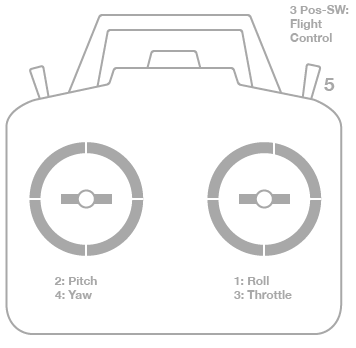
\includegraphics[width=0.5\linewidth]{radio_setup_mode_1}
	\centering
	\caption{\label{fig: mos_1}\textit{Transmitter(Mode 1): Recommended Channels}}
\end{figure}

\begin{figure}[h]
	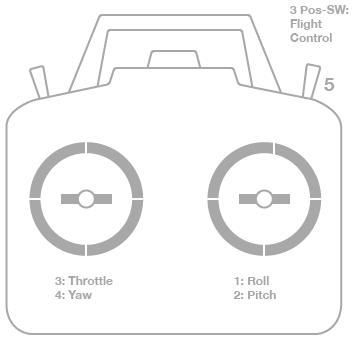
\includegraphics[width=0.5\linewidth]{rc_transmitter_mode2_setup}
	\centering
	\caption{\label{fig: mos_2}\textit{Transmitter(Mode 2): Recommended Channels}}
\end{figure}


\subsection{Channel Mappings}
Copter default channel mappings are:
\begin{itemize}
	\item \textbf{Channel 1}: Roll
	\item \textbf{Channel 2}: Pitch
	\item \textbf{Channel 3}: Throttle
	\item \textbf{Channel 4}: Yaw
	\item \textbf{Channel 5}: Flight Modes
	\item \textbf{Channel 6}: (Optional) Inflight tuning or camera mount (mapped to transmitter tuning knob)
\end{itemize}
Unused channels can be mapped to control additional peripherals.

\subsection{Connecting autopilot and turning on receiver}
We first connected the autopilot via USB and turned on your RC transmitter. Then, we verified that the transmitter is bound to the receiver (the receiver displayed a solid green light) and that it is set to use the correct model for our vehicle.

We then opened Mission Planner’s INITIAL SETUP | Mandatory Hardware | Radio Calibration screen. Since our RC receiver (Rx) and transmitter (Tx) are bound, we saw the green bars move when we moved the transmitter sticks.

\begin{figure}[h]
	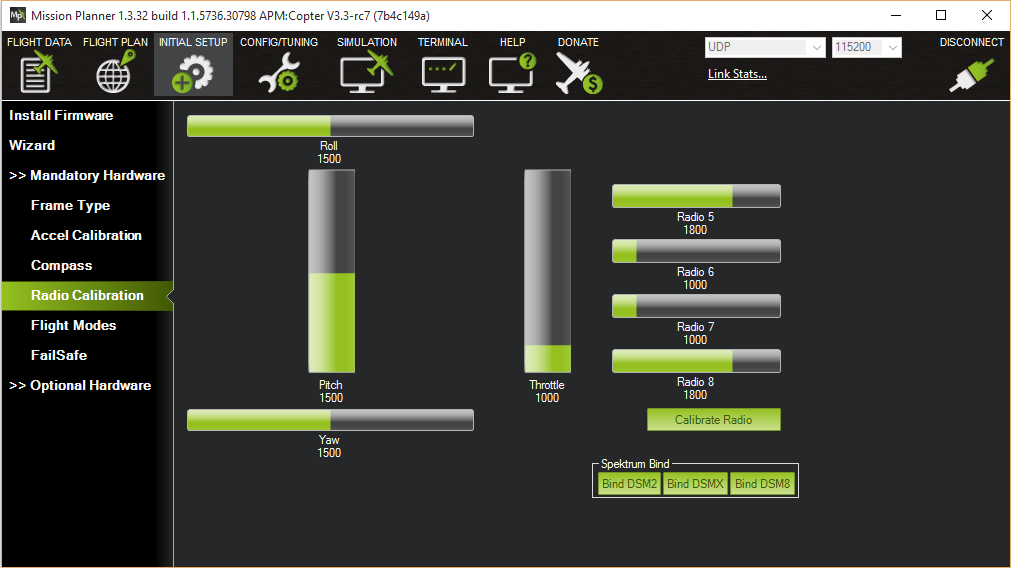
\includegraphics[width=1.0\linewidth]{mp_radio_calibration}
	\centering
	\caption{\label{fig: mos_3}\textit{MissionPlanner: Radio Calibration Screen (Copter)}}
\end{figure}

\subsection{Calibration steps}
\begin{enumerate}
	\item Opened Mission Planner’s INITIAL SETUP | Mandatory Hardware | Radio Calibration screen. A screen shown in Fig.~\ref{fig: mos_3} will be opened.
	\item Clicked on the green Calibrate Radio button in the lower right of the window.
Mission Planner displayed a prompt to check radio control equipment is on, battery is not connected, and propellers are not attached. We then selected OK. Screen shown in Fig.~\ref{fig: mos_4} will appear.
\begin{figure}[h]
	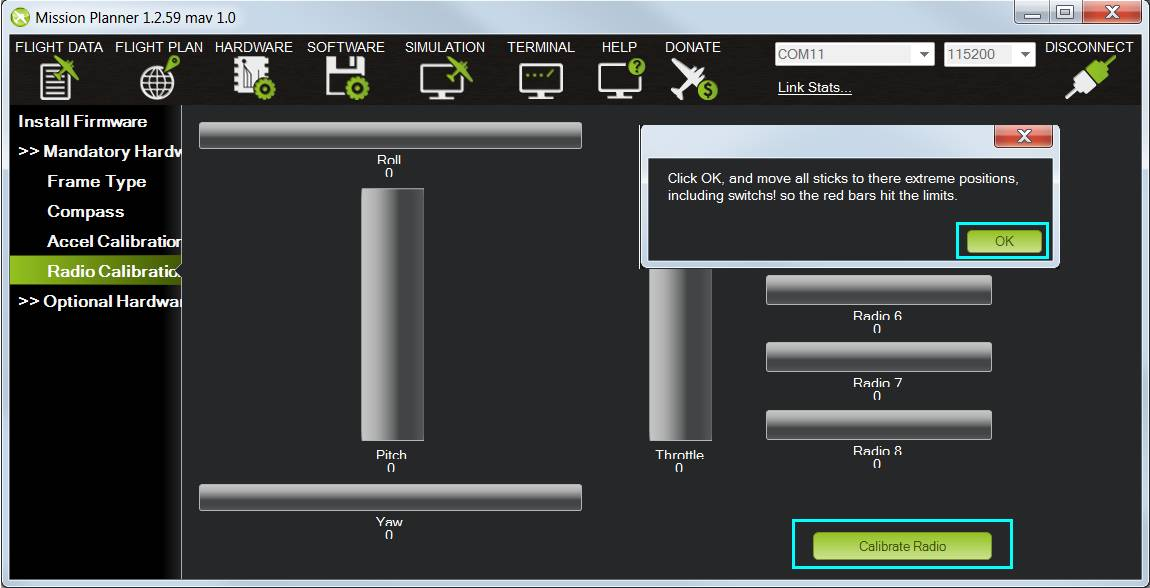
\includegraphics[width=1.0\linewidth]{mp_calibrate_radio}
	\centering
	\caption{\label{fig: mos_4}\textit{Mission Planner: Selected Calibrate Radio and then clicked OK to begin our calibration.}}
\end{figure}
	\item We then moved the control sticks and toggled switches on our transmitter to their limits of travel and observed the results on the radio calibration bars. Red lines appeared across the calibration bars to indicate maximum and minimum values:

\begin{figure}[h]
	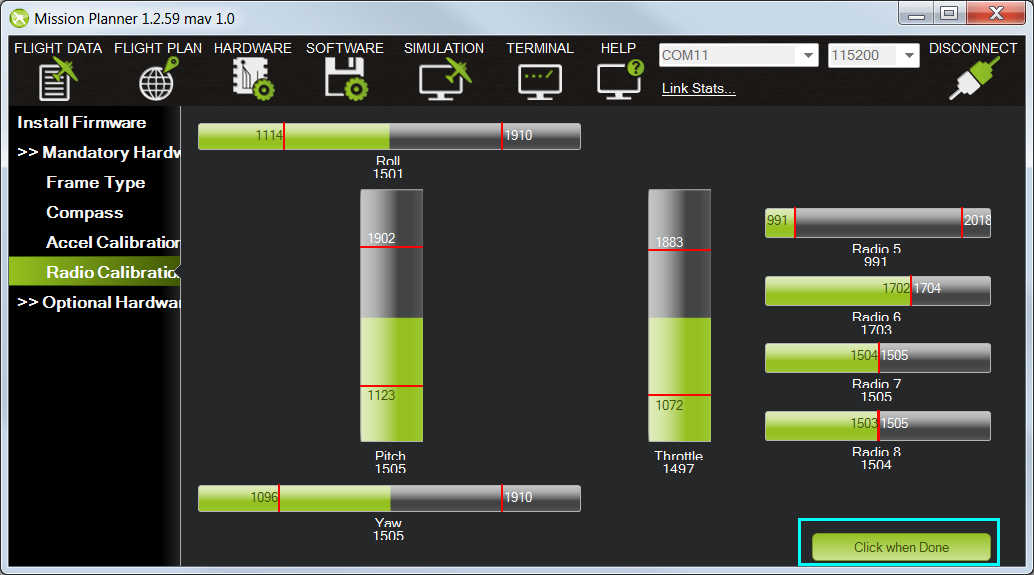
\includegraphics[width=1.0\linewidth]{mp_radio_calibration_click_when_done}
	\centering
	\caption{\label{fig: mos_5}\textit{Mission Planner: Input range marked with red lines}}
\end{figure}
\item Finally, we selected Click when Done when all required channels were set at the minimum and maximum positions.

Mission Planner showed a summary of the calibration data. Normal values are around 1100 for minimums and 1900 for maximums as shown in Fig.~\ref{fig: mos_5}.
\begin{figure}[h]
	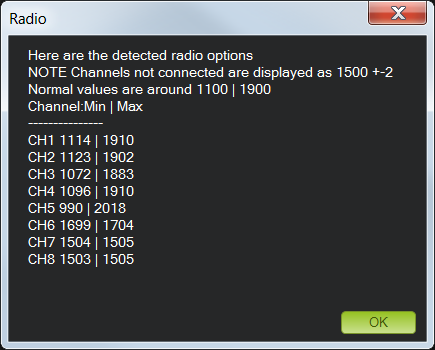
\includegraphics[width=0.7\linewidth]{radi-calib-results}
	\centering
	\caption{\label{fig: mos_6}\textit{Mission Planner: Radio Calibration Results}}
\end{figure}
\item Finally, we turned off our transmitter and disconnect the battery if it was connected and Radio Calibration results as shown in Fig.~\ref{fig: mos_6} appears.

\end{enumerate}

\subsection{RC Transmitter Flight Mode Configuration}
\subsubsection{Flight modes configuration}
The mapping between switch position and flight mode is set in the Mission Planner Flight Mode screen, as shown in Fig.~\ref{fig: mos_7}.

\begin{figure}[h]
	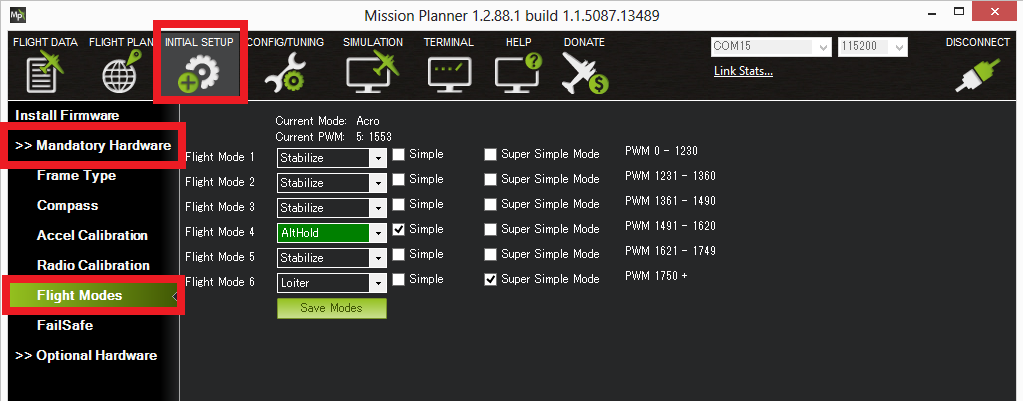
\includegraphics[width=1.0\linewidth]{mp_setup_flight_mode}
	\centering
	\caption{\label{fig: mos_7}\textit{Mission Planner:Flight Mode Screen}}
	\end{figure}
We set up the flight modes available on the transmitter by doing the following:
\begin{itemize}
	\item Turned on our RC transmitter
    \item Connected the APM 2.6 to the Mission Planner
	\item Went to the Initial Setup | Mandatory Hardware | Flight Modes screen
	\item Used the drop-down on each line to select the flight mode for that switch position.
	\item Ensured that at least one switch position is left assigned to STABILISE.
	\item Optionally checked the Simple Mode check-box for that switch position. 
	\item When finished, we pressed the Save Modes button.
	
	Some modes can also be invoked from the auxiliary switches (a.k.a. ch7, ch8 option switches). For example, to set a dedicated switch for RTL.
	
	
\end{itemize}

\subsubsection{Setting the flight mode channel}
The flight mode channel is the input radio channel that ArduPilot monitors for mode changes.
For our case, on our Copter this is always channel 5.

\subsubsection{Transmitter configuration}
The transmitter must emit PWM signals in the correct range to allow us to map a mode to a switch position.
If we wanted to just support three modes (using a three position switch) then we would configure the transmitter to produce PWM pulse widths of 1165, 1425, and 1815 microseconds for the respective switch positions.

If we want to support 6 modes then the transmitter will need to emit PWM widths of around 1165, 1295, 1425, 1555, 1685, and 1815 milliseconds. Typically this is achieved by configuring the transmitter to mix a two position switch and a three position switch (giving 6 modes in total). We can also do this with an analog dial if one is available, but it’s hard to reliably turn a dial to just the right position for six distinct settings.

The sections below provide links showing how to configure transmitters from different manufactures, and how to test (in Mission Planner) that each switch setting is emitting the appropriate PWM signal.

\subsubsection{Test transmitter switch settings}
We can use the Mission Planner Radio Calibration screen to test the PWM pulse widths for each mode setting.

We simply can toggle through the modes on our transmitter and confirm that the PWM for the selected channel matches the required PWM values. The screenshot in Fig.~\ref{fig: mos_8} assumes that the flight mode channel is set to Radio 5.



\begin{figure}[h]
	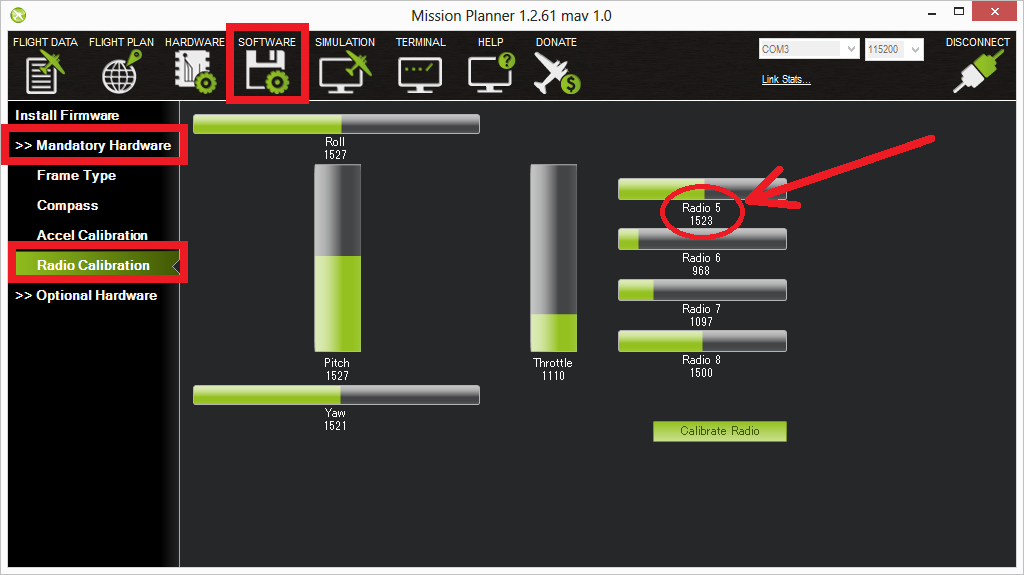
\includegraphics[width=1.0\linewidth]{mp_radio_calibration_ch5_pwm}
	\centering
	\caption{\label{fig: mos_8}\textit{Transmitter switch settings}}
\end{figure}


\section{Flight Modes and Autonomous Navigated Flight}
This section deals with the questions such as why did we end up with following flight modes and how did we went on about doing it.
\begin{itemize}
	\item Autotune Mode
	\item Stabilize Mode
	\item Loiter Mode
	\item RTL Mode
	\item Auto Mode (Autonomous flight)
\end{itemize}

\subsection{Autotune}

In order to get closer to our final aim of an autonomous flight, we needed a stabilized flight. For this, the PID values needed to be calibrated accordingly. Thus, we used this mode to autotune the paramters for a stable flight down the lane while using guided waypoints/auto mode, as shown in Fig.~\ref{fig: AutoTuneCh7Switch}.

AutoTune attempts to automatically tune the Stabilize P, Rate P and D, and maximum rotational accelerations to provide the highest response without significant overshoot. Copter needs to be “basically” flyable in Stabilize mode before attempting to use AutoTune as the feature needs to be able to “twitch” the copter in the roll and pitch axis.
\begin{figure}[h]
	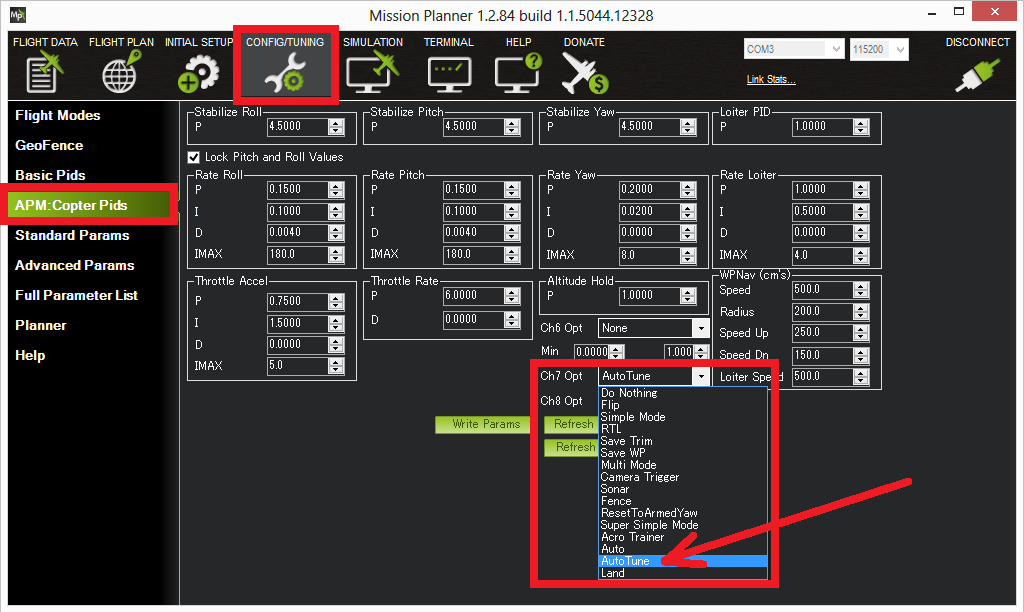
\includegraphics[width=1.0\linewidth]{AutoTuneCh7Switch}
	\centering
	\caption{\label{fig: AutoTuneCh7Switch}\textit{Setup for Autotune}}
\end{figure}

\subsubsection{Setup before flying}
\begin{enumerate}
	\item We set up one flight mode switch position to be AltHold/Stabilize.
	\item Then, we set an Auxiliary Function Switch to Autotune to allow us to turn the auto tuning on/off with the a switch.
\end{enumerate}
\subsubsection{How to invoke AutoTune}
\begin{enumerate}
	\item We waited for a calm day and went to a large open area.
	\item We then ensured that the ch7 or ch8 switch is in the LOW position.
	\item Took off and kept the copter into AltHold/Stabilize mode at a comfortable altitude.
	\item Faced the vehicle so that it will twitch at 90degrees from the direction the wind is blowing (i.e. if tuning Roll first, point the vehicle into the wind). Situation is explained graphically in Fig.~\ref{fig: autotune_copterwind}.
\begin{figure}[h]
	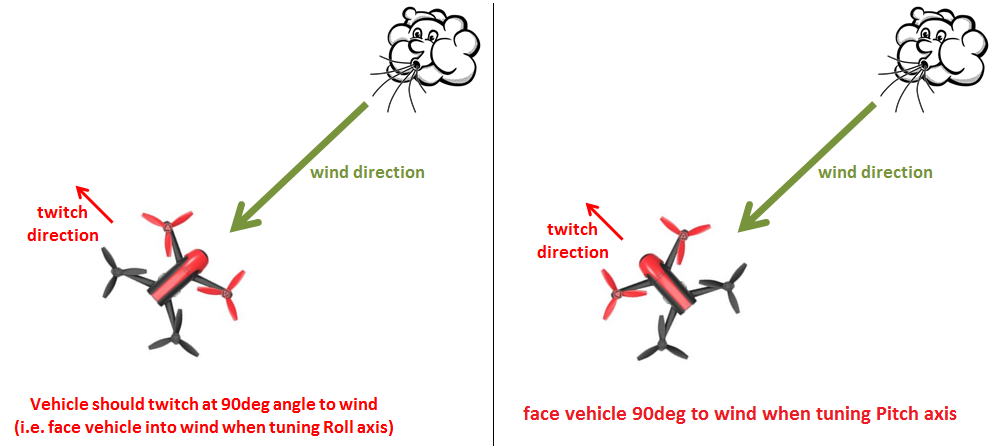
\includegraphics[width=1.0\linewidth]{autotune_copterwind}
	\centering
	\caption{\label{fig: autotune_copterwind}\textit{Twitch direction}}
\end{figure}
	\item Set the ch7/ch8 switch to the HIGH position to engage auto tuning:
	\begin{itemize}
		\item We will see it twitch about 20 degrees left and right for a few minutes, then it will repeat forward and back.
		\item We can use the roll and pitch stick at any time to reposition the copter if it drifts away (it will use the original PID gains during repositioning and between tests). When we release the sticks it will continue auto tuning where it left off.
		\item We can move the ch7/ch8 switch into the LOW position at any time to abandon the autotuning and return to the origin PIDs.
	\end{itemize}
	\item When the tune completes the copter will change back to the original PID gains.
	\item We can put the ch7/ch8 switch into the LOW position then back to the HIGH position to test the tuned PID gains.
	\item Feeling staisfied with the autotuned PID gains, left the ch7/ch8 switch in the HIGH position, landed and disarmed to save the PIDs permanently.
\end{enumerate}
We sometimes found that, after performing an AutoTune, that the vehicle feels overly twitchy when flying Stabilize, AltHold or PosHold (but ok in more autonomous modes like Loiter, RTL, Auto). For this, we tried reducing the RC\_FEEL parameter to $0.25$. This smooths out the given input.

\subsection{Stabilize Mode}
We focused on this mode for our application as this mode allows us to fly our vehicle manually, but self-levels the roll and pitch axis.

\subsubsection{Overview of this mode}
\begin{itemize}
	\item Pilot’s roll and pitch input control the lean angle of the copter. When we release the roll and pitch sticks the vehicle automatically levels itself.
	\item We would need to regularly input roll and pitch commands to keep the vehicle in place as it is pushed around by the wind.
	\item Our yaw input controls the rate of change of the heading. When we release the yaw stick the vehicle will maintain it’s current heading.
	\item Our throttle input controls the average motor speed meaning that constant adjustment of the throttle is required to maintain altitude. If the we put the throttle completely down the motors will go to their minimum rate (MOT\_SPIN\_ARMED) and if the vehicle is flying it will lose attitude control and tumble.
	\item The throttle sent to the motors is automatically adjusted based on the tilt angle of the vehicle (i.e. increased as the vehicle tilts over more) to reduce the compensation we must do as the vehicle’s attitude changes.
	
\end{itemize}
\subsubsection{Tuning}
 We used AutoTune which allowed us to automatically determine the best Stabilize and Rate PID values. 
 
Using this mode, after using the Autotune mode gave us an immense increase in the stability of the flight.



\subsection{Loiter Mode}
This mode was inculcated in our study to verify the first level of autonomy in our flight. This mode enabled us to verify the performance actually carried out by our system when shifted in autonomous mode. By verifying the working of this mode, it was safe for us to assume that we could shift over complete autonomy in guided waypoints mode where our copter flew to corresponding waypoints to achieve an autonomus flight.

Loiter Mode automatically attempts to maintain the current location, heading and altitude. A good GPS lock, low magnetic interference on the compass and low vibrations are all important in achieving good loiter performance.
\subsubsection{Controls}
We can control the copter’s position with the control sticks.

Horizontal location can be adjusted with the the Roll and Pitch control sticks with the default maximum horizontal speed being 5m/s (see Tuning section below on how to adjust this). When we release the sticks the copter will slow to a stop.
Altitude can be controlled with the Throttle control stick just as in AltHold/Stabilize mode
The heading can be set with the Yaw control stick
The vehicle can be armed in Loiter mode but only once the GPS has 3D lock and the HDOP has dropped below 2.0. 


\subsection{RTL Mode}
RTL mode (Return To Launch mode) was needed in our flight to navigate Copter from its current position to hover above the home position. So before/after completing the guided waypoint mission, we could direct our copter to RTL mode so that it may return and hover over the home location before ultimately landing. This mode basically gave control and stabilized our autonomous flight.
\subsubsection{Overview}
When RTL mode is selected, the copter will return to the home location. The copter will first rise to RTL\_ALT before returning home or maintain the current altitude if the current altitude is higher than RTL\_ALT. The default value for RTL\_ALT is 15m. We set it to 5m.

\begin{figure}[h]
	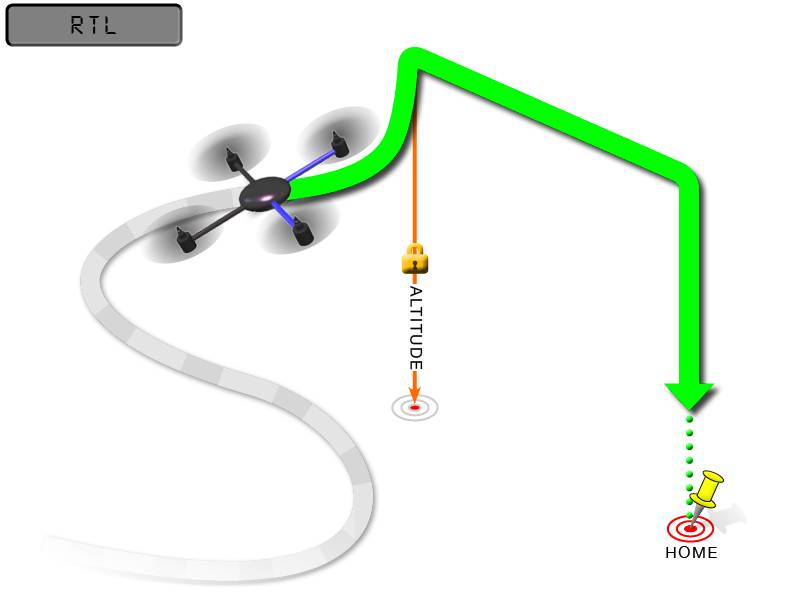
\includegraphics[width=0.7\linewidth]{RTL}
	\centering
	\caption{\label{fig: RTL}\textit{Return to Launch scenario}}
\end{figure}

RTL is a GPS-dependent move, so it was essential that GPS lock was acquired before attempting to use this mode. Before arming, we ensured that the APM’s blue LED is solid and not blinking (for confirmation of GPS fix). For a GPS without compass, the LED will be solid blue when GPS lock is acquired. For the GPS+Compass module, the LED will be blinking blue when GPS is locked(for our case). Figure ~\ref{fig: RTL} aptly describes the RTL Mode execution by our drone.

RTL commanded the copter to return to the home position, meaning that it will return to the location where it was armed. Therefore, the home position is always supposed to be our copter’s actual GPS takeoff location, unobstructed and away from people. For Copter if we get GPS lock and then ARM our copter, the home position is the location the copter was in when it was armed. This means if we execute an RTL in Copter, it will return to the location where it was armed. This is a needed mode while setting up the guided waypoints/Auto method.

\subsection{Auto Mode}
This is the actual mode which we were concerned for since beginning. This gave us the autonomy needed to inspect our crops efficiently and take images(data) by flying over them in a predefined path and taking videos/images using GoPro through a gimbal attached to our hex-copter. All the flight modes explained above were like a prerequisites needed to achive the success in this mode. 

In Auto mode the copter will follow a pre-programmed mission script stored in the autopilot which is made up of navigation commands (i.e. waypoints) and “do” commands (i.e. commands that do not affect the location of the copter including triggering a camera shutter). 
\subsubsection{Overview}
\begin{figure}[h]
	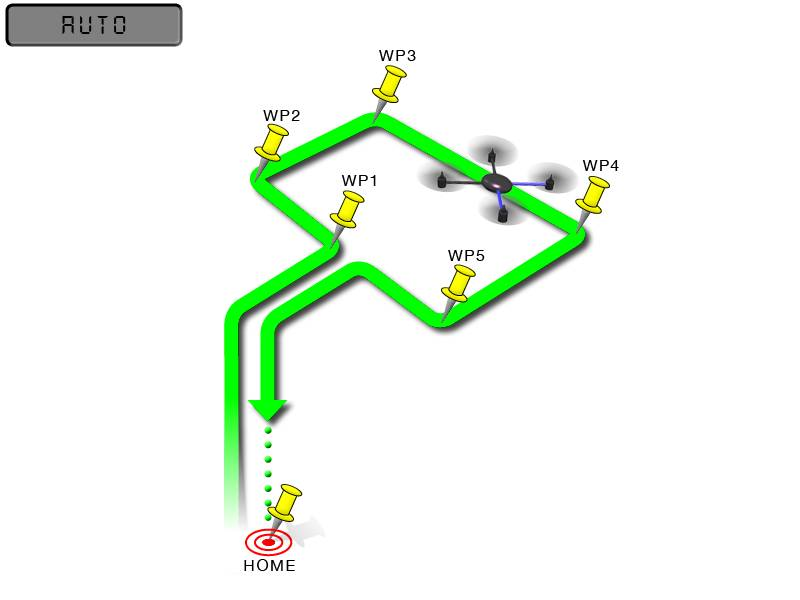
\includegraphics[width=0.7\linewidth]{auto}
	\centering
	\caption{\label{fig: auto}\textit{Overview of Auto Mode}}
\end{figure}
AUTO mode incorporates the altitude control from AltHold mode and position control from Loiter mode and should not be attempted before these modes are flying well as we mentioned above. All the same requirements apply including ensuring that vibration levels and compass interference levels are acceptable and that the GPS is functioning well including returning an HDOP of under 2.0. Figure ~\ref{fig: auto} aptly describes the Auto Mode execution.



\subsubsection{Controls and How it would be executed?}
AUTO should be set-up as one of the Flight Modes on the flight mode switch.

If starting the mission while the copter is on the ground wet should ensure the throttle is down, then we would switch to the Auto flight mode, then raise the throttle. The moment that the throttle is raised above zero, the copter will begin the mission.

If starting the mission from the air the mission will begin from the first command the moment that the flight mode switch is moved to Auto. If the first command in the mission is a take-off command but the vehicle is already above the take-off command’s altitude the take-off command will be considered completed and the vehicle will move onto the next waypoint.

At any time we can retake control (which was needed in our case many times due to poor GPS Connectivity) from the autopilot by returning the flight mode switch to another flight mode such as Stabilize or Loiter. If the pilot then switches to AUTO again, the mission will restart from the first command.

During the mission the our roll, pitch and throttle inputs are ignored but the yaw can be overridden with the yaw stick. This allows us to, for example aim the nose of the copter (which might have a hard mounted camera on it) as the copter flies the mission. The autopilot will attempt to retake yaw control as the vehicle passes the next waypoint. The overall Mission Flight Plan for the above explained Auto-Grid is shown in Fig.~\ref{fig: mp_auto_mission_grid}.

\subsubsection{Ending a Mission}

Missions should normally have an RTL as their final command to ensure the copter will return after the mission completes. Alternatively the final command could be a LAND with a different location. Without a final RTL or LAND command the copter will simply stop at the final waypoint and we will need to retake control with the transmitter.

We should remember that when using RTL, the copter will return to the “home” position which is the location where the copter was armed.

As the copter touches down at the end of the mission we should move the throttle to zero at which point the autopilot will disarm the motors if it also believes that it has landed.



There are detailed reasons why we utilized the above mentioned flight modes in our testing. 



 
\section{Conclusion}

We conducted some tests using the theory and practical approach mentioned earlier in this section. So we can conclude that using the apporach mentioned in this chapter which documented our way of planning a flight in the agricultural/farming area.

Following the approaches mentioned, we are trying to bridge the gap of open-source market with common people. We want to make the data available of crops from the agricultural field from flight data to the researcher's community so that all sorts of testing can be done on a large scale. Hence, we are planning to open source our image dataset we would be taking from an actual agricultural field following a mission as described in Fig.~\ref{fig: mp_auto_mission_grid}.



 % Image Data Collection using Autonomous Drone
	
	\chapter{Stitching of Images}

\section{About the Chapter}

The part of image processing in this project is to take the hyperspectral images from the drone and stitch them into a complete image of the farm for further analysis.

We require a well-structured dataset for the proper functioning of this system. The dataset consists of hyperspectral images order to get information about the image on a wider range of spectrum. The dataset should consist of a serial of overlapping images taken of the farm field in all four directions. Overlapping is an essential condition as we require it to increase the accuracy of image mosaicing. 



\begin{figure}[t]
	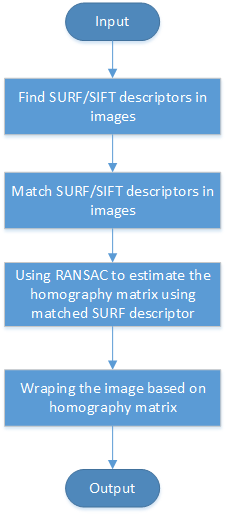
\includegraphics[height=0.9\linewidth]{extra-4}
	\centering
	\caption{\label{fig: extra-4}Image Mosaicing and Ortho-rectification process}
\end{figure}


\section{Image Mosaicing and Ortho-rectification}
The important steps in the algorithm are listed in Fig.~\ref{fig: extra-4} to give the reader an intuitive understanding.We need to stitch together our georeferenced images now to get an overall image of the farm land. This we can treat as the base map raster layer for our operations and we will perform a series of image processing algorithms on it to get pertinent data. The problem of image mosaicing is a combination of three problems:

\begin{enumerate}
	\item Correcting geometric deformations using image data and/or camera models.
	\item Image registration using image data and/or camera models.
	\item Eliminating seams from image mosaics.
\end{enumerate}

\subsection{Geometric corrections}
A geometric transformation could be a mapping that relocates image points. Transformations can be world or native in nature. Global transformations square measure sometimes outlined by a single equation that is applied to the complete image. Local transformations square measure applied to a half of image and those square measure tougher to specific briefly. 

The complications due to parallax that square measure determined within the case of change of location motion of a plate like camera are often avoided by employing a one dimensional camera to scan scenes. This action can be emulated victimization standard cameras by combining strips taken from a sequence of 2-D pictures as a series of neighboring segments. These cameras can directly acquire cylindrical (with a rotating motion) and writing (with change of location motion) maps. They can conjointly acquire pictures on Associate in nursing whimsical path. The strips that should be taken from 2-D pictures square measure known because the ones perpendicular to the image flow in. This family of strips can handle a wide form of motions together with motion and optical zoom. Additional formulation is developed in for these sophisticated cases of motion.

\section{Image Registration}
Image registration is the task of matching two or a lot of pictures. It has been a central issue for a range of problems in image process like seeing, monitoring satellite pictures, matching stereo images for reconstructing depth, matching biomedical pictures for designation, etc.

Registration is also the central task of image mosaicing procedures. The construction of mosaic images and the use of such images on several computer vision/graphics applications have been active areas of research in recent years. Carefully tag Associate in nursing pre-recorded camera parameters might be wont to eliminate the necessity for an automatic registration. User interaction also is a reliable supply for manually registering pictures (e.g. by choosing corresponding points and using necessary transformations on screen with visual feedback). Automated strategies for image registration used in image mosaicing literature will be categorized as follows:                                                                                                                                   

\begin{enumerate}
	\item Feature based methods
	\item Intensity based mosaicing
\end{enumerate}


\subsection{Feature based methods}

\begin{figure}[t]
	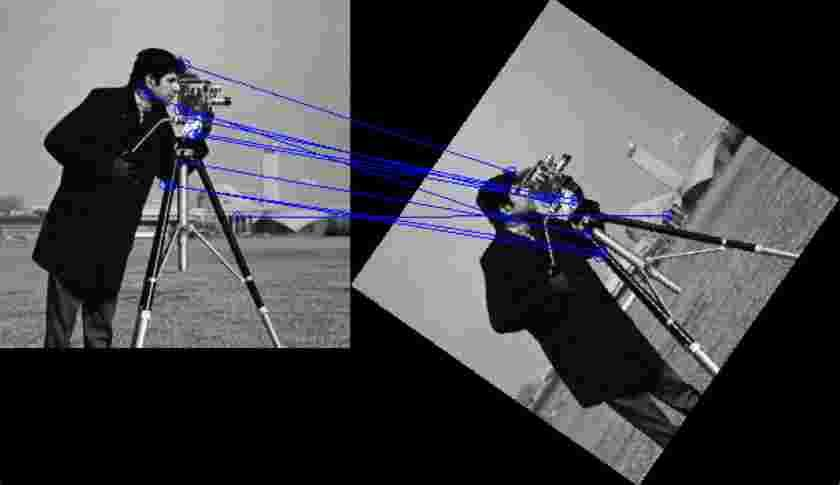
\includegraphics[width=0.9\linewidth]{extra-5}
	\centering
	\caption{\label{fig: extra-5}Feature based detection~\cite{FeatureD37:online}}
\end{figure}

In feature-based technique of Fig.~\ref{fig: extra-5}, all main feature points in an image pair is compare with all features in the other image by using one of the local descriptors. For image stitching based on feature-based techniques, feature extraction, registration, and blending are different steps required for doing image stitching. Feature-based methods are used by establishing correspondences between points, lines, edges, corners or any other shapes. The main characteristics of robust detectors includes invariance to image noise, scale invariance, translation invariance, and rotation transformations.

\subsection{Intensity based mosaicing}
Iteratively adjusting camera-motion parameters leads to local minimums unless a reliable initial estimate is provided. Initial estimates can be obtained using a coarse global search or an efficiently implemented frequency domain approach. Algorithm is as follows:

\begin{enumerate}
	\item For each pixel at ($x$, $y$) in the first image, we compute the corresponding pixel in the second image equal to ($x$', $y$').
	\item Compute the error density function between corresponding pixels.
	\item The problem is solved iterative to converge the error function towards the global minima.
\end{enumerate}

\section{Image Composting}
Images aligned once undergoing geometric corrections most seemingly need additional process to eliminate remaining distortions and discontinuities. Alignment of images might be imperfect as a result of registration errors ensuing from incompatible model assumptions, dynamic scenes, etc. Furthermore, in most cases images that want to be mosaiced don't seem to be exposed equally as a result of dynamical lighting conditions, automatic controls of cameras, printing/scanning devices, etc. These unwanted effects can be mitigated throughout the compositing method. 


The main downside in image compositing is that the problem of decisive however the pixels in Associate in nursing overlapping space ought to be delineated. Finding the best separation border between overlapping images has the potential to eliminate remaining geometric distortions. Such a border is likely to traverse around moving objects avoiding double exposure. The uneven exposure problem will be resolved by bar chart feat, by iteratively distributing the edge effect on the border to an outsized space, or by a smooth mixing perform.


\section{Ortho-Rectification of images}
The camera mounted on the drone is susceptible to different array of forces when the drone is airborne. This may result in changing of the orientation of the camera and hence the all the images may not be in the same plane. This can make the process of image mosaicing inaccurate and the final result we get will be a far off approximation of the real map of the field. To compensate for these errors, we need to implement some kind of pre-processing to account for this discrepancy in order to improve the efficiency of image mosaicing. Ortho-rectification is one of the ways to implement this compensation and is known to have good results for aerially acquired images. It is has an efficient implementation and so it requires less amount of processing time. This makes it compatible for real-world processing systems which is great advantage.
\begin{figure}[t]
	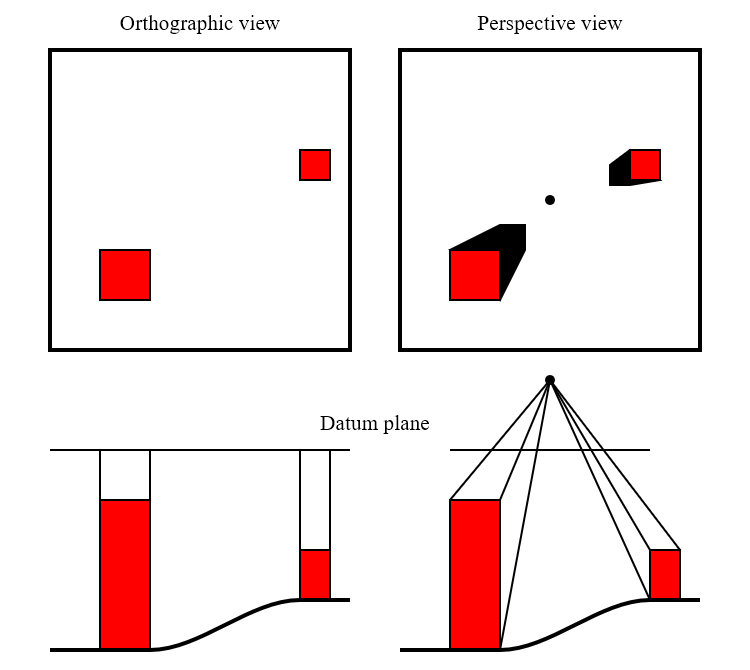
\includegraphics[height=0.9\linewidth]{extra-6}
	\centering
	\caption{\label{fig: extra-6}Ortho Rectification~\cite{OrthoPer57:online}}
\end{figure}
The process of ortho-rectification of Fig.~\ref{fig: extra-6} involves mapping of via aircraft non-inheritable pictures on a map of a similar size victimisation many geo-reference management points (GCPs)~\cite{1}. The topographical variations in the surface of  the world and also the tilt of the camera have an effect on  the gap with that options on the aerial image area unit show. The more topographically various the landscape, the more distortion inherent in the photograph. As a result, real world distances don't seem to be represented uniformly on the photograph. For example in a very steep area would relate to a way longer distance than an inch measured over a flat surface like a visible. Ortho-rectification is the name of the method accustomed removes these sources of distortion to equilibrate pic units with world distances. Once an aerial pic has been ortho-rectified, it is commonly cited as associate degree ortho-photo. A fascinating facet note is whereas ortho-rectification removes horizontal distortion; vertical relief displacement continues to be maintained. For example, the sides of a building would still contain distortion.

In some cases, a simple rectification method like removing the consequences of the lean of the camera is also all that's necessary. This is very rare and in most cases a lot of concerned method is needed. After removing the impact of the camera tilt, removing the effects of relief should be accomplished by knowing the elevation of the piece of land higher than (or below) the mapping plane must be identified~\cite{4}.

\subsection{Methods used in ortho-rectification}
There are two ways by that rectification of associate degree aerial photograph will occur. In the first case, Ground Control Points (GCP) are determined either typical ground surveys, from published maps, by Global Positioning System (GPS) surveys, or by aero triangulation. These points are taken at visible physical options on the landscape. On the corresponding image, the $x$, $y$ photo coordinates are then determined for every corresponding GCP. Depending on the sort of recursive correction to be used, a minimum of 3 to five GCP should be established. The relationship of the x, y photo coordinates to the real world GCP is then wont to confirm the algorithmic program for resampling the image.

The second method of ortho-rectification is to use DEMs. These elevations are collected from stereoscopic models by photogrammetric ways to kind a digital elevation model (DEM). As with using GCPs, the mathematical relationship between the real worlds coordinates and also the scanned aerial photograph is set and also the digital image is resampled to form the rectified image. For both cases, the resampling of the digital image involves warping the image thus that distance and space are uniform in relationship to world measurements. This means that with the resampled image, an in. on the image currently measures an equivalent distance on steep tract because it will during a field. Depending the on the desires of the aerial mental imagery within the GIS system, there are blessings and disadvantages to mistreatment either technique. GCP ortho-rectification is a faster method and may be accomplished mistreatment existing paper maps to ascertain the GCPs. Using DEMs for ortho-rectification is a lot of correct method by that to geocode digital mental imagery however need associate degree existing DEM or DTM for process. Once an image has been ortho-rectified it is often used with vector and formation information of an equivalent organization. This image can currently have broad outlines and street names overlay onto it. As mentioned before, spatial information will additionally currently be accurately measured in terms of distances and space, allowing for a lot of advanced spatial analysis~\cite{4}.

All the above mentioned method work separately for image mosaicing and ortho-rectification. We can use the SIFT (Scale Invariant Feature Transform) and SURF (Speeded-Up Robust Features) algorithms to simultaneously ortho-rectify the images and also stitch them. 

\section{SIFT and SURF}

\subsection{SIFT Detector}
\begin{figure}[h]
	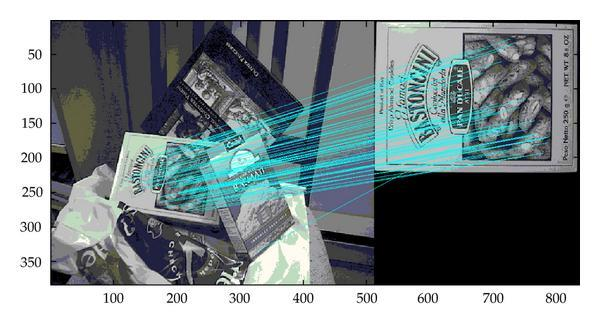
\includegraphics[width=0.9\linewidth]{extra-7}
	\centering
	\caption{\label{fig: extra-7}SIFT Based feature detection~\cite{FeatureM52:online}}
\end{figure}
Lowe proposed the Scale Invariant Feature remodel (SIFT). It has four computational phases that includes: scale-space extrema detection, key-point localization, orientation assignment, and defining key-point descriptors. The first stage is to spot location and scales of key point’s exploitation scale house extrema within the DoG (Difference-of-Gaussian) functions. In the key point localization Fig.~\ref{fig: extra-7} step, key point candidates are localized and refined by eliminating the key points wherever they rejected the low distinction points. In the orientation assignment step, the orientation of key point is obtained primarily based on native image gradient. In key-point descriptors stage, SIFT computes the local image descriptor for every key purpose supported image gradient magnitude and orientation at every image sample purpose in a very region focused at key purpose. These samples build a $3D$ histogram of gradient location and orientation, with $4$ X $4$ array location grid and eight orientation bins in each sample. SIFT provides a $128$-element dimension of key point descriptor. 

\subsection{SURF Detector}

The Speed-up Robust Feature detector (SURF) rule is based mostly on multiscale area theory and Speeds-up its computations by quick approximation of boot matrix and descriptor exploitation ``integral images''. SURF uses three feature detection steps namely; detection, description, and matching. SURF speeded-up the SIFT’s detection process by keeping in read of the standard of the detected points Fig.~\ref{fig: extra-8}. It gives a lot of focus on speeding-up the matching step~\cite{5}. The Hessian matrix is used alongside descriptors low spatial property to considerably increase the matching speed. SURF is widely used in the pc vision community. SURF has proven its potency and hardiness in the invariant feature-localization. 
\begin{figure}[h]
	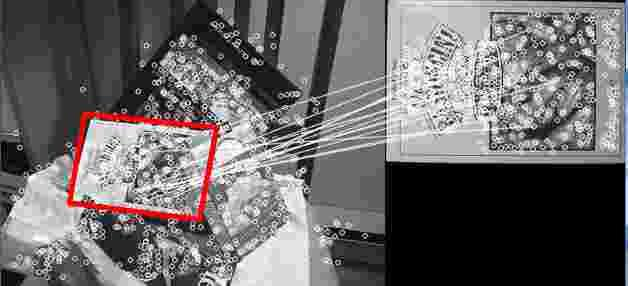
\includegraphics[width=0.9\linewidth]{extra-8}
	\centering
	\caption{\label{fig: extra-8}SURF Based feature based detection~\cite{FeatureD76:online}}
\end{figure}

\section{OpenDronemap based Image Processing}

OpenDroneMap is a tool to postprocess drone, balloon, kite, and street view data to geographic data including orthophotos, point clouds, \& textured mesh.

Docker is the world’s leading software container platform. Developers use Docker to eliminate ``works on my machine'' problems when collaborating on code with co-workers. Using containers, everything required to make a piece of software run is packaged into isolated containers. Unlike VMs, containers do not bundle a full operating system - only libraries and settings required to make the software work are needed.

We used opendronemap to achieve the step of image stitching robustly. We used docker as a container for easier installation and cross-platform support across all different OS and platforms. 

The main command to start the procedure is:

\begin{lstlisting}
docker build -t opendronemap:latest
\end{lstlisting}

This command builds the docker image using dockerfile. This command also creates a container that is used to generate the stitched image using georef coordinates.

\begin{lstlisting}
`docker run -it --rm -v img_loc:/code/images -v odm_orthophoto:/code/odm_orthophoto -v 
/odm_texturing:/code/odm_texturing my_odm_image_2`
\end{lstlisting}


 % Stitching of Images
	
	\chapter{Analysis of Stitched Image}

\section{About}
Analysis on the stitched image formed from previous steps is an important part of the system. This analysis helps to derive useful insights from the image which is used to provide prescription to the farmers.
This chapter describes the usgae of analysis techniques like Vegetation Indices as a measure of crop health combined with machine learning algorithms for better prediction. Classification of images taken by the farmer, with the use of deep learning is also dicussed. 
 
\section{Comparison of Different Image Analysis Techniques}
Given a framework that gathers the necessary data, the decision making to be performed requires knowledge extraction from these data. Hyperspectral images contain a lot of useful information that can be analyzed to generate many insightful results. These results can then help to produce a reliable prescription map and present the solutions in a way that can be understood by the farmers.

Over the years, a number of Vegetation Indices (VIs) have been developed by combining two or more wavebands in the hyperspectral images in ratios and/or differences, to highlight various crop conditions. However, one of the problems in applying VIs to crop yield estimation is the difficulty in choosing the most appropriate vegetation index in a specific situation (Barrett and Curtis 1999). In fact, various environmental factors, such as background effects and crop canopy conditions, have been shown to be potential sources of noise, which affect the spectral reflectance in canopy level (Aparicio et al., 2000). Ironically, these difficulties, to identify the most useful wavelengths or VIs under specific environmental conditions, have been heightened with the recent proliferation of large volume of data available from hyperspectral and broadband sensors. Sensitivity of vegetation indices and tapping the full potential of large quantities of spectral information acquired with the latest sensors are currently the most important impediments to successfully applying remote sensing technologies to precision farming.

Artificial intelligence and especially machine learning have contributed to the creation of control systems in agriculture. Machine learning is the process of discovering previously unknown and potentially useful information from data. It is one of the most important and useful data mining tools that can discover unknown regularities and patterns from data sets. There are a lot of machine learning algorithms like Support Vector Machines(SVM), Simple Multivariate Linear Regressions(SMLR), Decision Trees(DT), Neural Networks(NN), etc. available that can be utilized for recognizing intricate patterns in data. Implementation of these algorithms in agricultural domain have shown inspiring results as shown in Table ~\ref{tab: tab1}.
 
\begin{figure}[t]
	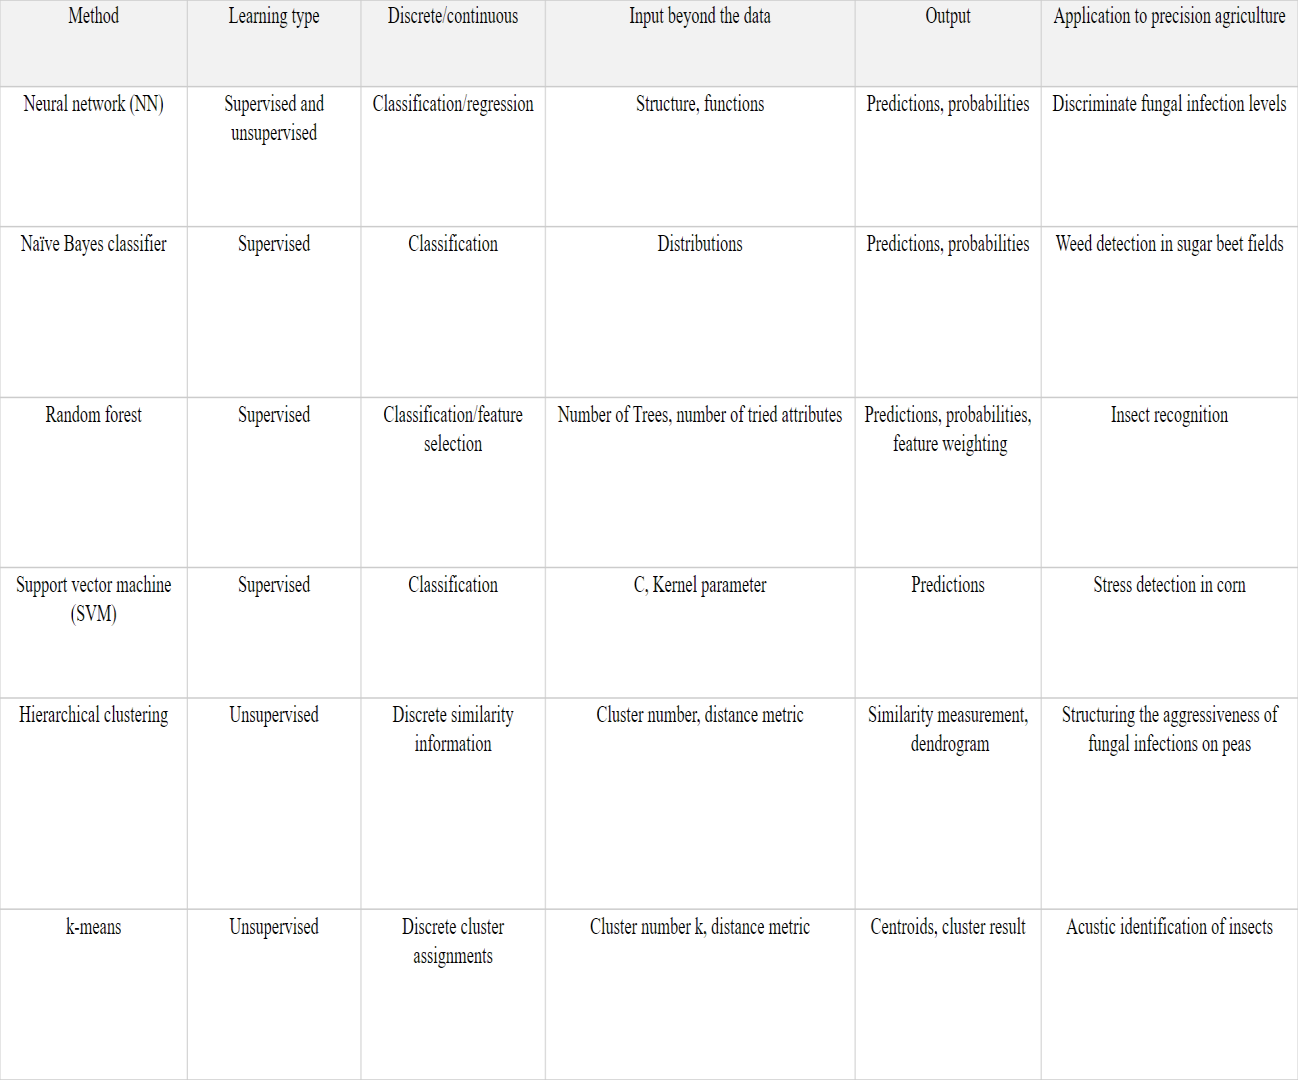
\includegraphics[width=1\linewidth]{extra-9}
	\centering
\captionof{table}{Comparison between different machine learning algorithms along with their application in agricultural domains} \label{tab: tab1}
\end{figure}

Deep Neural Networks (DNNs), have generated a strong interest in their potential effectiveness in estimating various field and crop conditions. The ability of DNNs to associate complicated information with target attributes without any constraints for sample distribution, make them ideal for describing the intricate and complex non-linear relationships which exist between canopy-level spectral signatures and various crop condition. In fact, successful applications have already been reported for surface water quality assessment, soil moisture estimation, biomass estimation, and yield prediction. A Deep Neural Network (DNN) is a computational model which mimics the human nervous system and decision-making process. Although some technical difficulties, such as the low interpretability of the developed models, the complexity involved in optimizing the model structure, and the high processing power required for the training process, once made the intensive application of this techniques difficult, recent improvements in computing power and learning algorithms has increased the applicability of the method in various fields.

A combination of VI methods, mainly Normalized Differnce Vegetation Index(NDVI) and machine learning is used as a part of analysis on hyperspectral data. This requires a lot of labelled dataset but due to its unavailablity we needed to generate our own data. Figure~\ref{fig: dada} shows the flow of the algorithm as used by us to generate labellled data and train the SoftMax model. NDVI calculations are done on the stitched image whose output is then fed into the K-means clustering algorithm to generate labelled data. This labelled data is then used to train the SofMax regression model. 
\begin{figure}[h]
	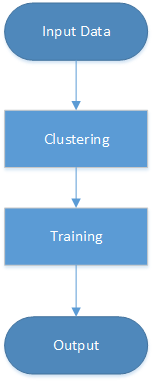
\includegraphics[height=1.0\linewidth]{dada}
	\centering
	\caption{\label{fig: dada}Flowchart to generate labelled data and train machine learning model}
\end{figure}


Evaluation of a new stitched image of the farm is done using this SoftMax model to determine critical areas on the farm which are shown by different colors on the output image which is overlaid on Google Map. Once the critical areas are determined we can go a step ahead to analyse the problem in those areas on the farm. The widespread distribution of smartphones among crop growers around the world with an expected 5 billion smartphones by 2020 offers the potential of turning the smartphone into a valuable tool for diverse communities growing food. To derive the potential of this fact along with the abilities of deep learning, we trained a deep learning model to recognize diseases in crops. The farmer can go to the critical areas on the farm and take a photograph of infected crops which will be evaluated against our deep learning model to provide a prescription.



\section{Image Analysis Using Indexing}

The hyperspectral images we have carry vital information that can be analyzed to deduce important parameters about crops. VI based methods provide many ways to explore this using specific algorithms designed to perform analysis on such images. Some of those which we wish to use are Normalized Difference Vegetation Index (NDVI), to know the chlorophyll content in leaves. A flowchart of the process is shown in Fig.~\ref{fig: extra-10}.

\begin{figure}[h]
	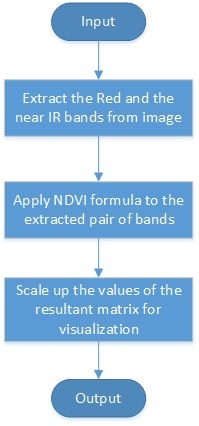
\includegraphics[height=0.9\linewidth]{extra-10}
	\centering
	\caption{\label{fig: extra-10}Image analysis using VI based methods}
\end{figure}


\subsection{Normalized Difference Vegetation Index}

The Normalized Difference Vegetation Index (NDVI) is a numerical indicator that uses the visible and near-infrared bands of the spectrum, and is adopted to analyze remote sensing measurements and assess whether the target being discovered contains live inexperienced vegetation or not. NDVI has found a wide application in vegetative studies because it has been accustomed estimate crop yields, pasture performance, and rangeland carrying capacities among others. It is often directly associated with different ground parameters like percentage of ground cowl, photosynthetic activity of the plant, surface water, leaf  area index and the quantity of biomass. NDVI was first used in 1973 by Rouse et al. from the Remote Sensing Centre of Texas A$\&$M University.

Generally, healthy vegetation will absorb most of the visible lightweight that falls on that, and reflects a large portion of the near-infrared lightweight. Unhealthy or sparse vegetation reflects additional visible lightweight and fewer near-infrared lightweight. Bare soils on the different hand mirror moderately in each the red and infrared portion of the spectrum. Since we recognize the behavior of plants across the spectrum, we will derive NDVI info by specializing in the satellite bands that area unit most sensitive to  vegetation info (near-infrared and red). The bigger the distinction so between the near-infrared and therefore the red coefficient, the more vegetation there has to be. The NDVI algorithm subtracts the red reflectance values from the near-infrared and divides it by the sum of near-infrared and red bands.

\begin{equation} \label{eq: eq-1}
NDVI = (NIR-RED)/(NIR+RED)
\end{equation}
This formulation allows us to cope with the fact that two identical patches of vegetation could have different values if one were, for example in bright sunshine, and another under a cloudy sky. The bright pixels would all have larger values, and therefore a larger absolute difference between the bands. This is avoided by dividing by the sum of the reflectance. 

\begin{figure}[h]
	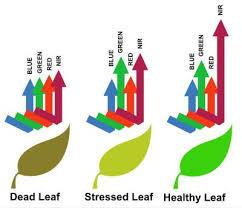
\includegraphics[height=0.5\linewidth]{fin_img_8}
	\centering
	\caption{\label{fig: reflectance}Reflectances from different types of leaves}
\end{figure}

Theoretically, NDVI values are represented as a ratio ranging in value from -1 to 1 but in practice extreme negative values represent water, values around zero represent bare soil and values over 0.6 represent dense green vegetation. Reflectances from different types of leaves is shown in Fig.~\ref{fig: reflectance}.


\subsection{Clustering and Classification}
After all the index calculations are done we are left with areas with different discrete patches that may have the same index range. The next step would be to cluster the similar data (pixel values) into a single color coded areas. The clustering is done using K-means algorithm. This clustered information is then used to train a SoftMax regression model for classification of new images as mentioned previously.

\subsubsection{K-means Algorithm}
K-means is one of the best unsupervised learning algorithms that solve the well-known bunch downside. Initially number of centers, which is k, is decided according to the Elbow Rule which minimizes the cost function with an appropriate number of clusters. The main idea is to outline kcenters, one for each cluster. These centers should be placed in a crafty method attributable to totally different location causes different result. So, the better selection is to put them the maximum amount as potential secluded from one another.

The next step is to assign the closest center to each data point. At this point we'd like to recalculate k new centroids as center of mass of the clusters ensuing from the previous step. After we have a tendency to have these k new centroids, a new binding must be done between constant data set points and therefore the nearest new center. A loop has been generated. As a result of this loop we could notice that the k centers amendment their location step by step till no additional changes square measure done or in different words centers don't move from now on. Finally, this algorithm aims at minimizing associate objective operate is aware of as square error operate given by:


\begin{equation} \label{eq: eq-3}
J(V) = \sum_{i=1}^{C}\sum_{j=1}^{C_i} (\begin{Vmatrix}x_i-v_i
\end{Vmatrix})^2
\end{equation}
\begin{equation*} 
\begin{Vmatrix}x_i-v_i

\end{Vmatrix} \text{is the Euclidean distance between } x_i \quad \& \quad v_j 
\end{equation*}
\begin{equation*} 
c_i \text{ is the number of data points in the $i_{}^{th}$ cluster}
\end{equation*}
\begin{equation*} 
c \text{ is the number of cluster centers}
\end{equation*}


Algorithmic steps for k-means clustering:

Let $X = \begin{Bmatrix} x_1,x_2,x_3,...,x_n \end{Bmatrix}$ be the set of data points and $V = \begin{Bmatrix} v_1,v_2,v_3,...,v_c \end{Bmatrix}$ be the set of centers.

\begin{enumerate}
	\item Randomly select ‘c’ cluster centers.
	\item Calculate the distance between each data point and cluster centers.
	\item Assign the data point to the cluster center whose distance from the cluster center is minimum of all the cluster centers.
	\item Recalculate the new cluster center using,
	\begin{equation} \label{eq: eq-4}
	v_i = (1/C_i)  \sum_{j=1}^{C_i}x_i
	\end{equation}
	where $c_i \text{ represents the number of data points in the $i_{}^{th}$ cluster}$
	\item Recalculate the distance between each data point and new obtained cluster centers.
	\item If no data point was reassigned then stop, otherwise repeat from step 3.	
\end{enumerate}


\subsection{Softmax Regression Model}
Once we have  labelled data we can train a machine learning model for better analysis of the farm. In our case we employ the use of SoftMax regression model to learn the range of NDVI values. Softmax regression is a generalization of logistic regression to the case where we want to handle multiple classes. It is a regression model which generalizes the logistic regression to classification problems where the output can take more than two possible values. SoftMax regression is competitive in terms of CPU and memory consumption. The Softmax Regression is preferred when we have features of different type (continuous, discrete, dummy variables etc), nevertheless given that it is a regression model, it is more vulnerable to multicollinearity problems and thus it should be avoided when our features are highly correlated. The structural architecture of the algorithm is shown in Fig.~\ref{fig: softmax}.
\begin{figure}[t]
	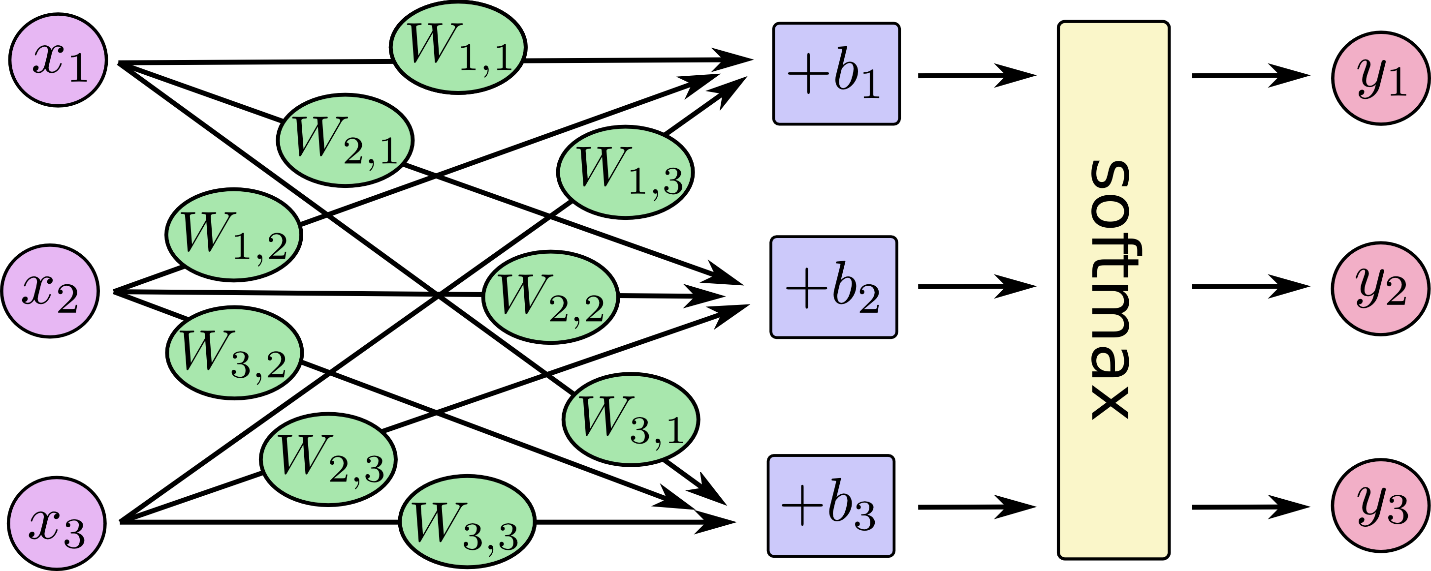
\includegraphics[width=1.0\linewidth]{fin_img_11}
	\centering
	\caption{\label{fig: softmax}Basic structure of Softmax Model}
\end{figure}

This model divides the input farm image into different color coded regions depending upon the NDVI values.This image is then overlayed onto the Google Map for better visualization of the farm. This image shows critical areas on the farm which can further be analysed for crop disease prediction using deep learning.


 % Analysis of Stitched Image
	
	\chapter{Crop Disease Prediction using Deep Learning}

\section{About}
Crop diseases are a major threat to food security, but their rapid identification remains difficult in many parts of the world due to the lack of the necessary infrastructure. The combination of increasing global smartphone penetration and recent advances in computer vision made possible by deep learning has paved the way for smartphone-assisted disease diagnosis. Using a public dataset~\cite{PlantVil94:online} of 54,306 images of diseased and healthy plant leaves collected under controlled conditions, we train a deep convolutional neural network to identify 14 crop species and 26 diseases (or absence thereof). Once the color coded image is overlaid on the Google Map, the farmer can go to the critical areas and click pictures of the unhealthy crops. These images will be evaluated against our already trained model and a prescription would be presented to the farmer on the application.

\section{Deep Learning Model}
Deep learning is a branch of machine learning based on a set of algorithms that attempt to model high level abstractions in data. In a simple case, you could have two sets of neurons: ones that receive an input signal and ones that send an output signal. When the input layer receives an input it passes on a modified version of the input to the next layer. In a deep network, there are many layers between the input and output (and the layers are not made of neurons but it can help to think of it that way), allowing the algorithm to use multiple processing layers, composed of multiple linear and non-linear transformations~\cite{deng2009imagenet}.

Many deep learning architectures such as Deep Neural Networks(DNNs), Convolutional Neural Networks(CNNs), and Recurrent Neural Networks(RNNs) have shown to produce state-of-the-art results on various tasks~\cite{ehler2006integrated}. As a powerful visual model, CNNs have demonstrated remarkable performance in various visual recognition problems, and attracted considerable attention in recent years.

The performance of convolutional neural networks in object recognition and image classification has made tremendous progress in the past few years. ~\cite{hughes2015open}, ~\cite{facts2015figures}, ~\cite{jia2014caffe}, ~\cite{krizhevsky2012imagenet} and ~\cite{lecun1989backpropagation}. Previously, the traditional approach for image classification tasks has been based on hand-engineered features such as SIFT~\cite{lecun2015deep}, HoG~\cite{lin2013network}, and then to use some form of learning algorithm in these feature spaces. This led to the performance of all these approaches depending heavily on the underlying predefined features. Feature engineering itself is a complex and tedious process which needed to be revisited every time the problem at hand or the associated dataset changed considerably. This problem has occurred in all traditional attempts to detect plant diseases using computer vision as they leaned heavily on hand-engineered features, image enhancement techniques, and a host of other complex and labour-intensive methodologies. 

\subsection{Convolutional Neural Networks}
Convolutional Neural Networks are very similar to ordinary Neural Networks, they are made up of neurons that have learnable weights and biases. Each neuron receives some inputs, performs a dot product and optionally follows it with a non-linearity. The whole network expresses a single differentiable score function: from the raw image pixels on one end to class scores at the other. And they have a loss function (e.g. SVM/Softmax) on the last (fully-connected) layer. CNN architectures make the explicit assumption that the inputs are images, which allows us to encode certain properties into the architecture. These then make the forward function more efficient to implement and vastly reduce the amount of parameters in the network~\cite{CS231nCo51:online}.


Neural Networks receive an input (a single vector), and transform it through a series of hidden layers. Each hidden layer is made up of a set of neurons, where each neuron is fully connected to all neurons in the previous layer, and where neurons in a single layer function completely independently and do not share any connections. The last fully-connected layer is called the ``output layer'' and in classification settings it represents the class scores, as it can be seen in Fig.~\ref{fig: extra-12} and Fig.~\ref{fig: extra-13}. Convolutional Neural Networks take advantage of the fact that the input consists of images and they constrain the architecture in a more sensible way. In particular, unlike a regular Neural Network, the layers of a CNN have neurons arranged in 3 dimensions: width, height, depth. 

\begin{figure}[h]
	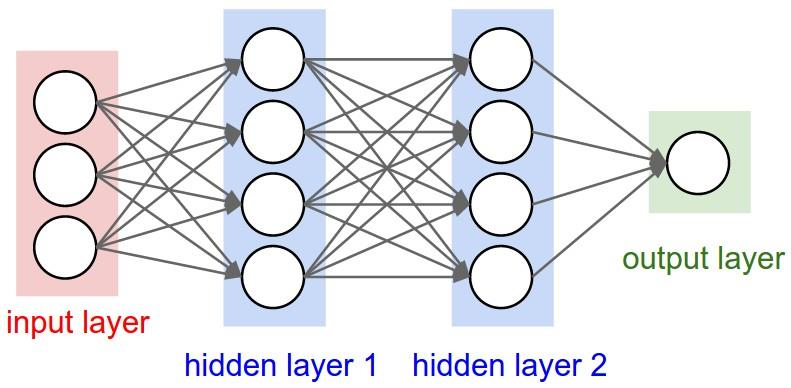
\includegraphics[width=1\linewidth]{extra-12}
	\centering
	\caption{\label{fig: extra-12}A regular 3-layer Neural Network~\cite{CS231nCo51:online}}
\end{figure}
\begin{figure}[h]
	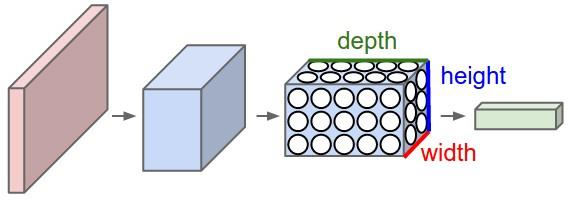
\includegraphics[width=1\linewidth]{extra-13}
	\centering
	\caption{\label{fig: extra-13}A CNN arranges its neurons in three dimensions (width, height, depth), as visualized in one of the layers. Every layer of a CNN transforms the 3D input volume to a 3D output volume of neuron activations. In this example, the red input layer holds the image, so its width and height would be the dimensions of the  image, and the depth would be 3 (Red, Green, Blue channels)~\cite{CS231nCo51:online}}
\end{figure}


A simple CNN is a sequence of layers, and every layer transforms one volume of activations to another through a differentiable function. We use three main types of layers to build CNN architectures: Convolutional Layer, Pooling Layer, and Fully-Connected Layer. In this way, CNNs transform the original image layer by layer from the original pixel values to the final class scores. 


\subsection{Deep Learning Frameworks}
Deep learning methods have resulted in significant performance improvements in several application domains and as such several software frameworks have been developed to facilitate their implementation to foster research and development in artificial intelligence. We can leverage these open-source tools and frameworks to implement many complex algorithms for different applications. Some of the very common frameworks include Caffe, Neon, TensorFlow, Theano, Torch, etc. 

Deep learning generally means building large scale neural networks with many layers. Simply put, these networks are simply functions which generate outputs Y given inputs X. In addition to the input X, the functions make use of a bunch of parameters (also called weights). These can include scalar values, vectors, and most expensively, matrices and higher-order tensors. A tensor is just a generalization of vectors and matrices into higher dimensions. The particular functions in vogue today involve tens of computationally expensive linear algebra operations, including matrix products and convolutions. Before we can train the network, we define a loss function. Common loss functions include squared error for regression problems and cross-entropy loss for classification. To train a network, we need to successively present many batches of new inputs to the network. After each is presented, we update the model by taking the derivative of the loss with respect to all of our parameters. So right away there are a few obvious problems. First, multiplying tens or hundreds or tensors together millions of times to process even a moderately sized dataset is terribly expensive. Second, taking the derivative of giant ugly functions by hand is a pain and could consume days or weeks that would be better spent imagining new experiments. This is why we need libraries like Theano, Caffe, Torch, and TensorFlow. The takeaway here is first that with any of these libraries you can write only the prediction code or forward pass and the framework will figure out how to take derivatives for you, that is to calculate the backwards pass. Second, you write your code once in a nice high-level language without ever learning the ugly details of GPU coding, and the framework will compile for whatever CPU or NVIDIA hardware you have access to.


\subsubsection{Why TensorFlow?}
TensorFlow is an open source software library by Google for numerical computation using data flow graphs. Nodes in the graph represent mathematical operations, while the graph edges represent the multidimensional data arrays (tensors) communicated between them. The flexible architecture allows us to deploy computation to one or more CPUs or GPUs in a desktop, server, or mobile device with a single API. The best part is that we can build every algorithm using easy to use data flow graphs which helps to visualize our algorithm’s architecture. TensorFlow seems to have a faster compile time and its computational graphs can be distributed on a cluster for computations. TensorFlow is both an R\&D and deployment framework. Support from such a huge company as Google is a big advantage for TensorFlow. TensorFlow can work with any gradient-based machine learning algorithm, which opens up a much broader range of uses. Written in C++ for speed, it doesn't require the developer to know anything about the underlying hardware. It also runs across multiple devices and architectures, so it's intended to scale from SoC devices, like phones, all the way up to distributed systems using dozens of GPUs. The main barrier to using any framework for math, statistics, or machine learning is ease-of-use. Likewise, one of TensorFlow's proffered advantages is ease-of-use. 

\textbf{Features:}


\begin{itemize}
	\item Multi GPU support
	\item Training across distributed systems
	\item Visualize the graphs using TensorBoard
	\item Model checkpointing
\end{itemize}


A few years ago, AlexNet~\cite{hughes2015open} showed for the first time that end-to-end supervised training using a deep convolutional neural network architecture is a practical possibility even for image classification problems with a very large number of classes, beating the traditional approaches using hand-engineered features by a substantial margin in standardbenchmarks. The absence of the labor-intensive phase of feature engineering and the generalizability of the solution makes them a very promising candidate for a practical and scalable approach for computational inference of plant diseases. Google also released its deep learning model GoogLeNet~\cite{szegedy2015going} in 2014 similar to AlexNet. Among the AlexNet and GoogLeNet architectures, GoogLeNet consistently performs better than AlexNet~\cite{mohanty2016using}, and based on the method of training, transfer learning always yields better results~\cite{mohanty2016using}, both of which were expected. An application of the ``network in network'' architecture~\cite{prince2015automatic} in the form of the inception modules is a key feature of the GoogleNet architecture.

In this report we used the concept of transfer learning to fine-tune the final layer of Google’s Inception V-3 (GoogLeNet) model based upon TensorFlow.

\subsection{Transfer Learning}
Modern object recognition models have millions of parameters and can take weeks to fully train. Transfer learning is a technique that shortcuts a lot of this work by taking a fully-trained model~\cite{pan2010survey} for a set of categories like ImageNet, and retrains from the existing weights for new classes. Transfer learning provides the opportunity to adapt a pre-trained model to new classes of data with several advantages. A basic concept of transfer learning is shown in Fig.~\ref{fig: transfer}.

\begin{figure}[h]
	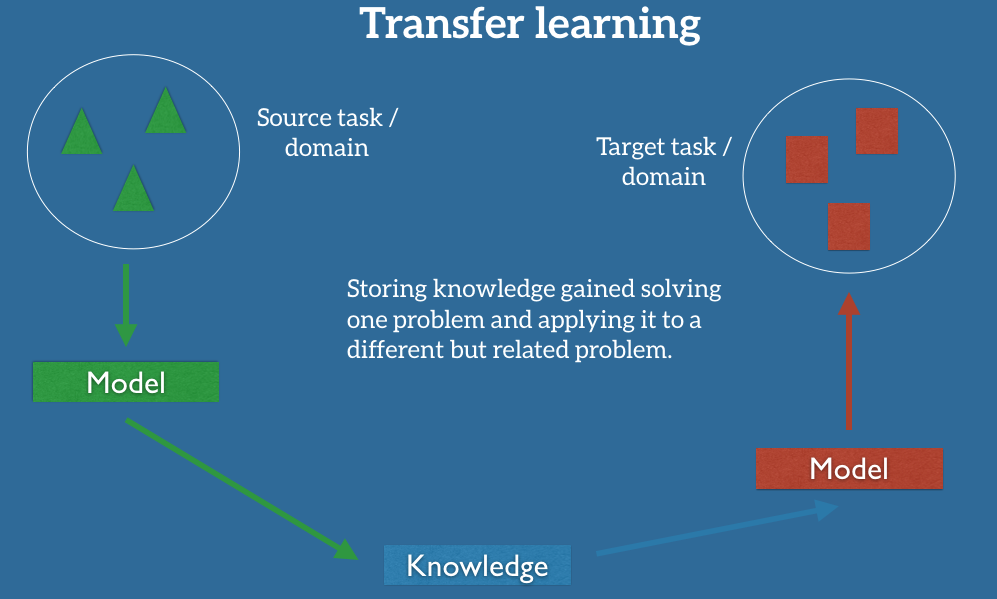
\includegraphics[width=1\linewidth]{fin_img_13}
	\centering
	\caption{\label{fig: transfer}Transfer Learning setup}
\end{figure}

In practice, we seek to transfer as much knowledge as we can from the source setting to our target task or domain. This knowledge can take on various forms depending on the data: it can pertain to how objects are composed to allow us to more easily identify novel objects; it can be with regard to the general words people use to express their opinions, etc. 

\subsubsection{Inception V-3 model}
Inception v3 is the 2015 iteration of Google’s Inception architecture for image recognition trained upon ImageNet data. Inception is a really great architecture and it’s the result of multiple cycles of trial and error.
 
Inception is basically:
\begin{itemize}
	\item An 299x299x3 input representing a visual field of 299 pixels
	and 3 color (RGB) channels
	\item Five vanilla convolution layers, with a few interspersed max-
	pooling operations
	\item Successive stacks of ``Inception Modules''
	\item A softmax ouput layer at the end ( logits ) and at an intermediate 	output layer ( aux\_logits ) just after the mixed 17x17x768e layer.
\end{itemize}


\begin{figure}[h]
	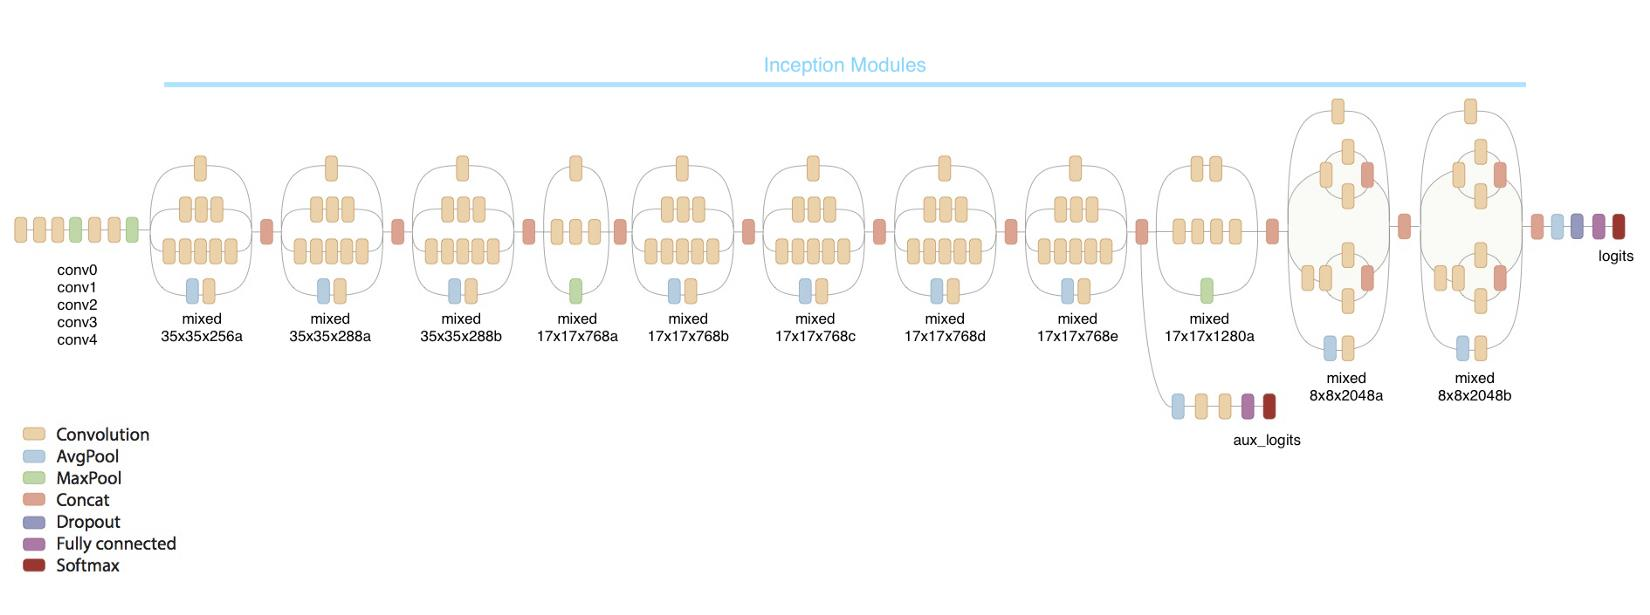
\includegraphics[width=1\linewidth]{fin_img_14}
	\centering
	\caption{\label{fig: inception}Overview of inception architecture~\cite{arxivorg71:online}}
\end{figure}




It’s the repeated stacking of the Inception modules that makes this architecture deep. While stacking Inception modules leads to depth, each module is also wide and architected to recognize features at multiple length scales. Overview of inception architecture is shown in Fig.~\ref{fig: inception}.











 % Crop Disease Prediction using Deep Learning
	
	\chapter{Experimental Results}

We hereby present the results of the experiments concluded so far. It includes the results of the autonomous flight of the hex-copter used for collection of data, image stitching using ODM library, NDVI analysis using QGIS and crop disease prediction using Google's inception v-3 model. A step wise flow of the web portal describing these steps is also shown for better understanding.

\section{Autonomous flight for data collection}

Stability of the hex-copter is increased by tuning the PID paramters by Autotune mode and thereby checking in Loiter mode as described below.

\subsection{Verifying Loiter performance with dataflash logs}
Viewing the loiter’s horizontal performance is best done by downloading a dataflash log from our flight, then open it with the mission planner and graph the NTUN message’s DesVelX vs VelX and DesVelY vs VelY. In a good performing copter the actual velocities will track the desired velocities as shown in Fig.~\ref{fig: Loiter_TuningCheck}, X = latitude (so positive = moving North, negative = South), Y = longitude (positive = East, negative = West).

\begin{figure}[h]
	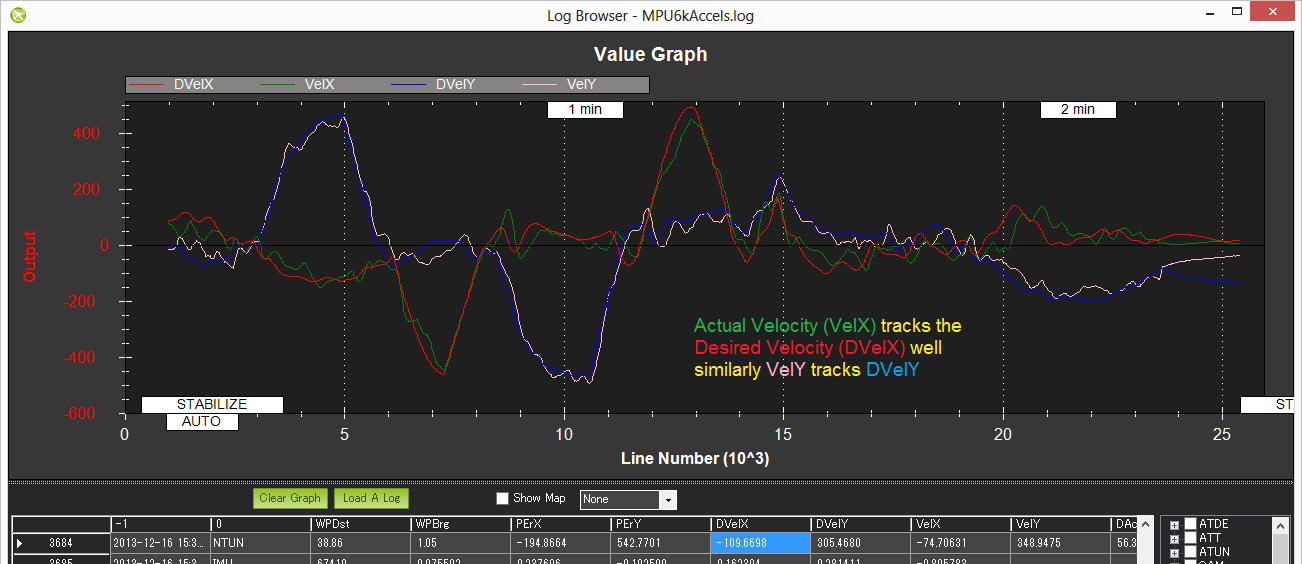
\includegraphics[width=1.0\linewidth]{Loiter_TuningCheck}
	\centering
	\caption{\label{fig: Loiter_TuningCheck}\textit{Loiter Mode Tuning Check using dataflash logs}}
	\end{figure}

\subsection{Verifying performance with dataflash logs}
Viewing the stabilize mode performance is best done by downloading a dataflash log from our flight. We opened it with the mission planner and graph the ATT message’s Roll-In or DesRoll (pilot desired roll angle) vs Roll (actual roll) and Pitch-In or DesPitch (desired pitch angle) vs Pitch (actual pitch angle). These two should track well as shown in Fig.~\ref{fig: Tuning_StabilizeCheck} for our flight test.
\begin{figure}[h]
	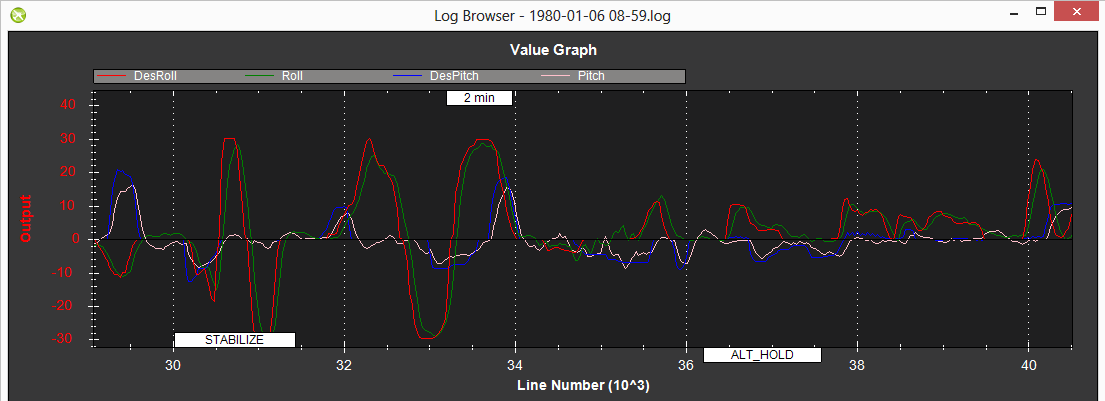
\includegraphics[width=1.0\linewidth]{Tuning_StabilizeCheck}
	\centering
	\caption{\label{fig: Tuning_StabilizeCheck}\textit{Stability Check using dataflash logs}}
\end{figure}

Some flight tests for autonomous flight have been conducted where we achieved the success of flying the flight in the modes mentioned above with considerably great stability. The images of some flight tests are shown in Fig.~\ref{fig: auto_self_I} and Fig.~\ref{fig: auto_self_II}.


\begin{figure}[h]
	\hfill
	\subfigure[]{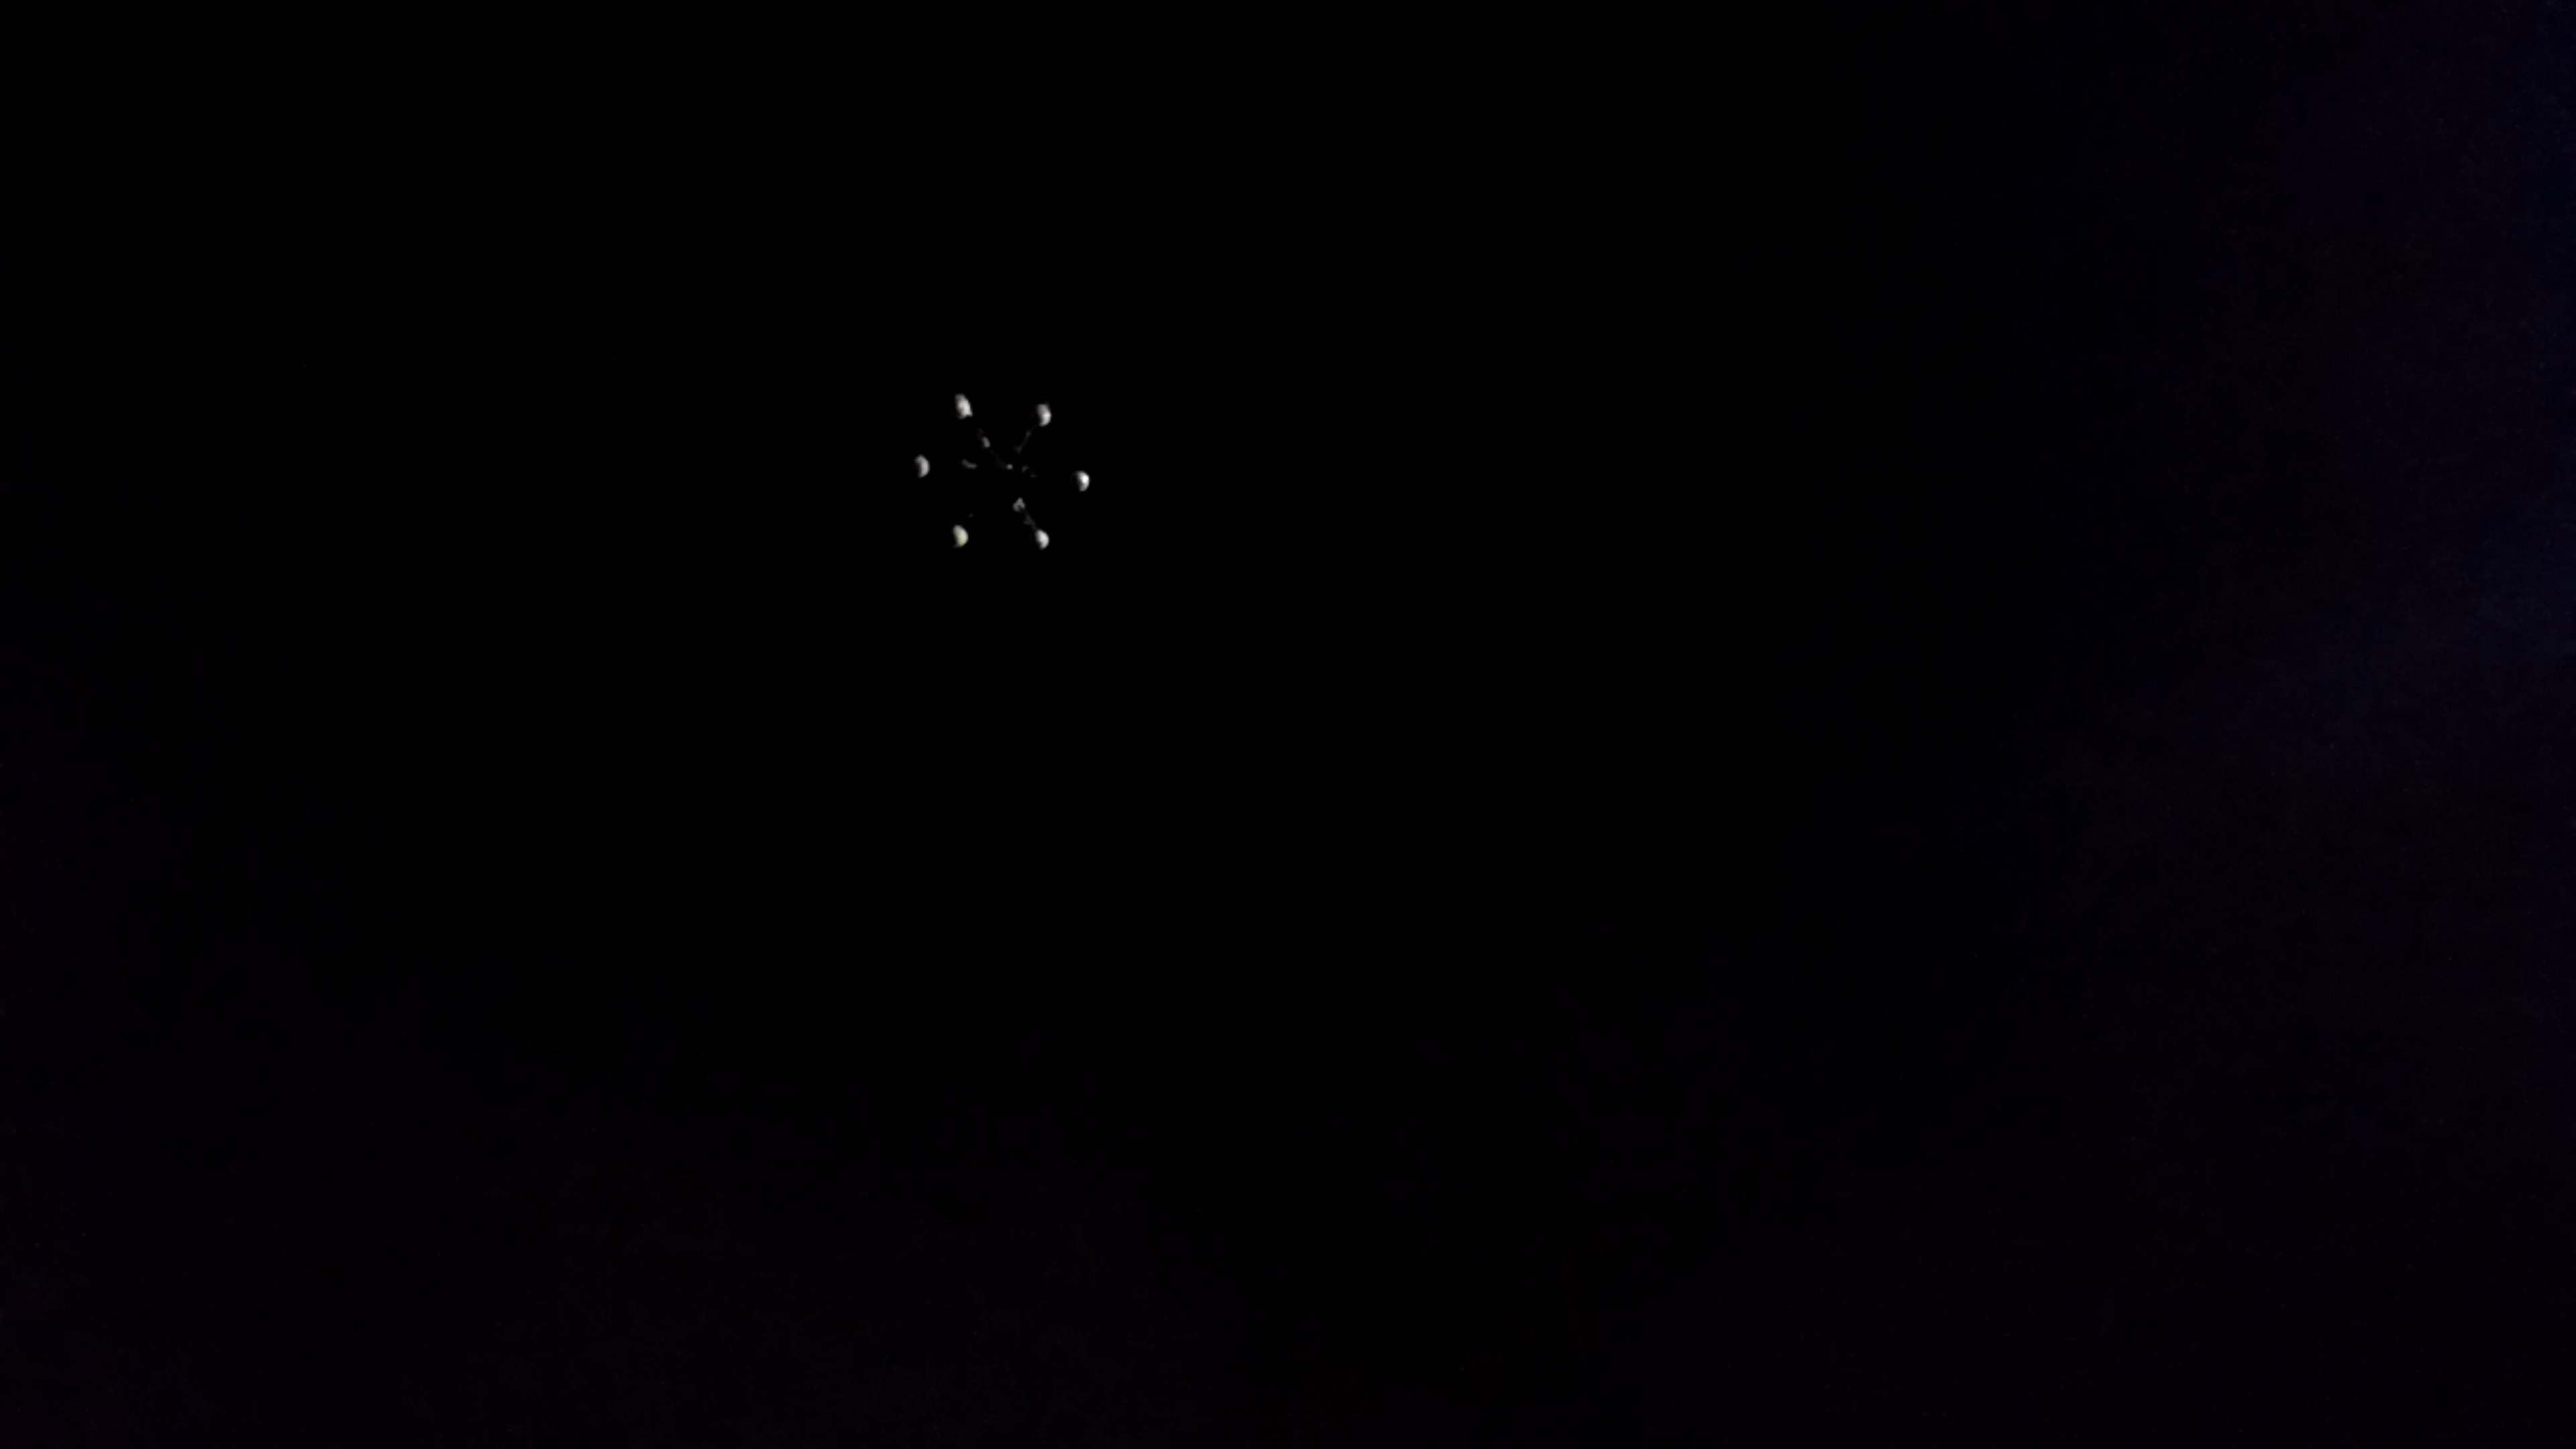
\includegraphics[width=0.48\linewidth]{auto_self_1}}
	\hfill
	\subfigure[]{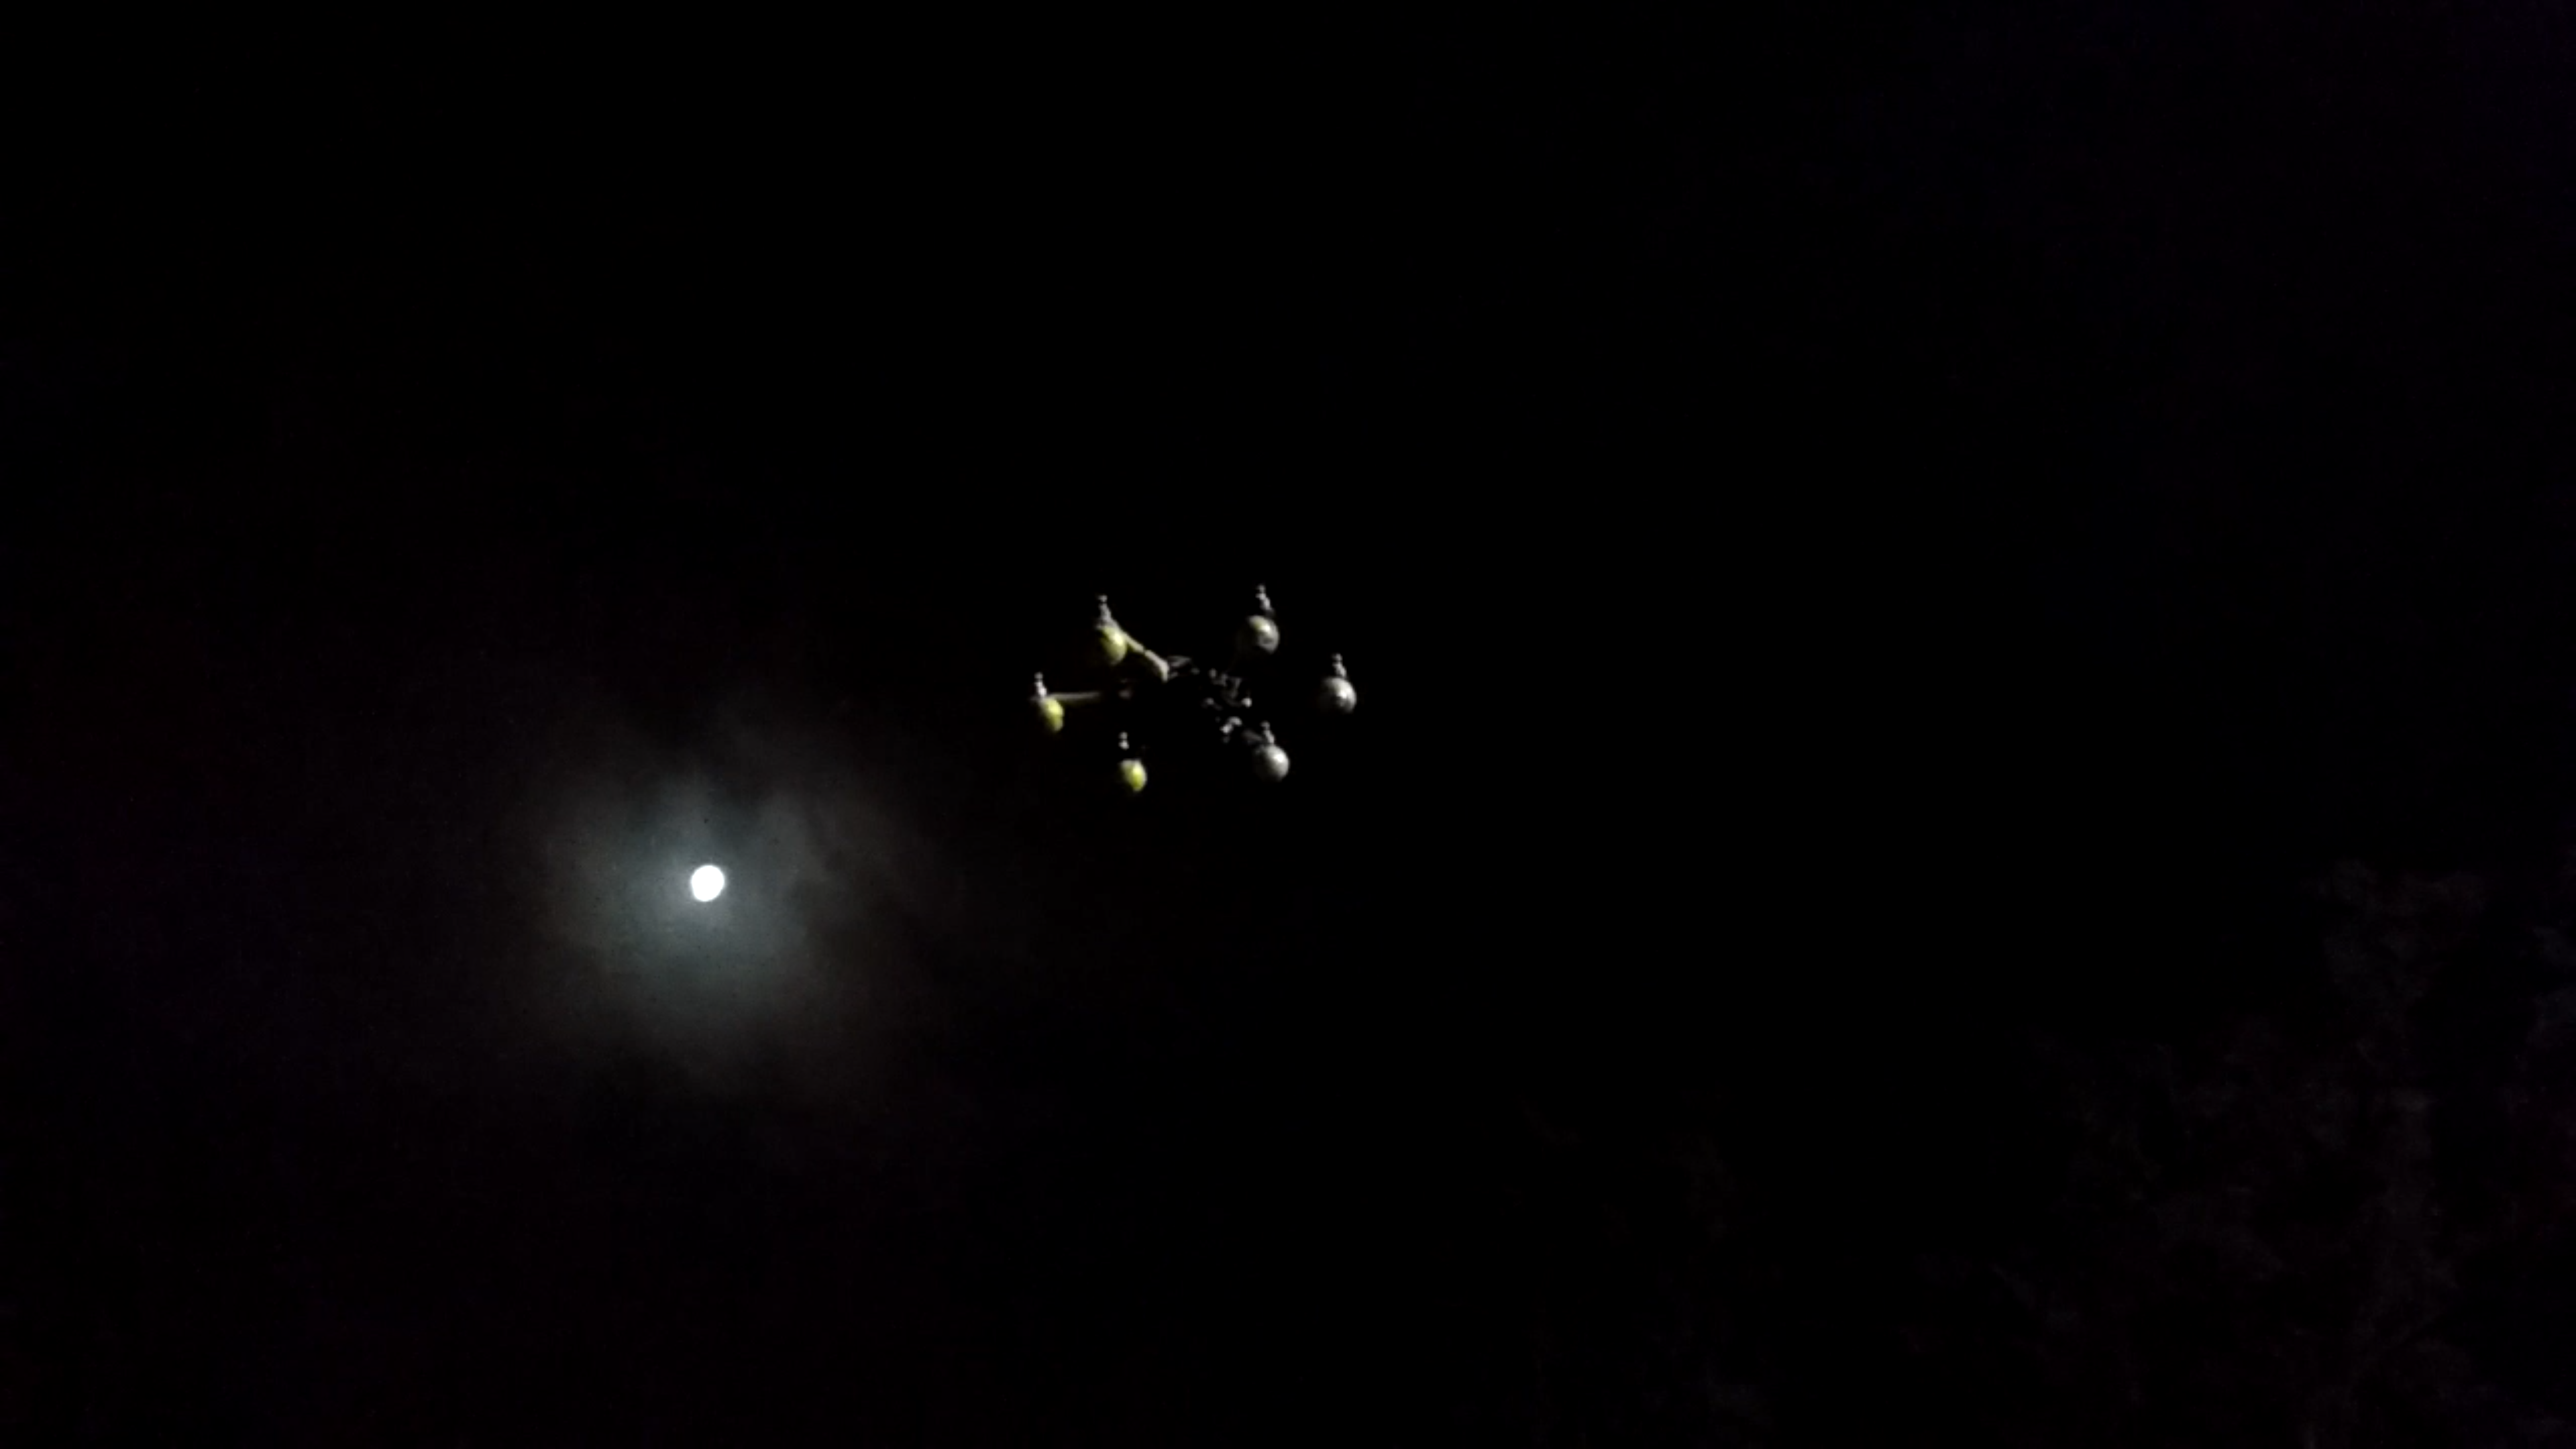
\includegraphics[width=0.48\linewidth]{auto_self_2}}
	\hfill
	\caption{\label{fig: auto_self_I}Flight test data (images) taken during night at Old CRC Lawns in SVNIT Campus}
\end{figure}

\begin{figure}[h]
	\hfill
	\subfigure[]{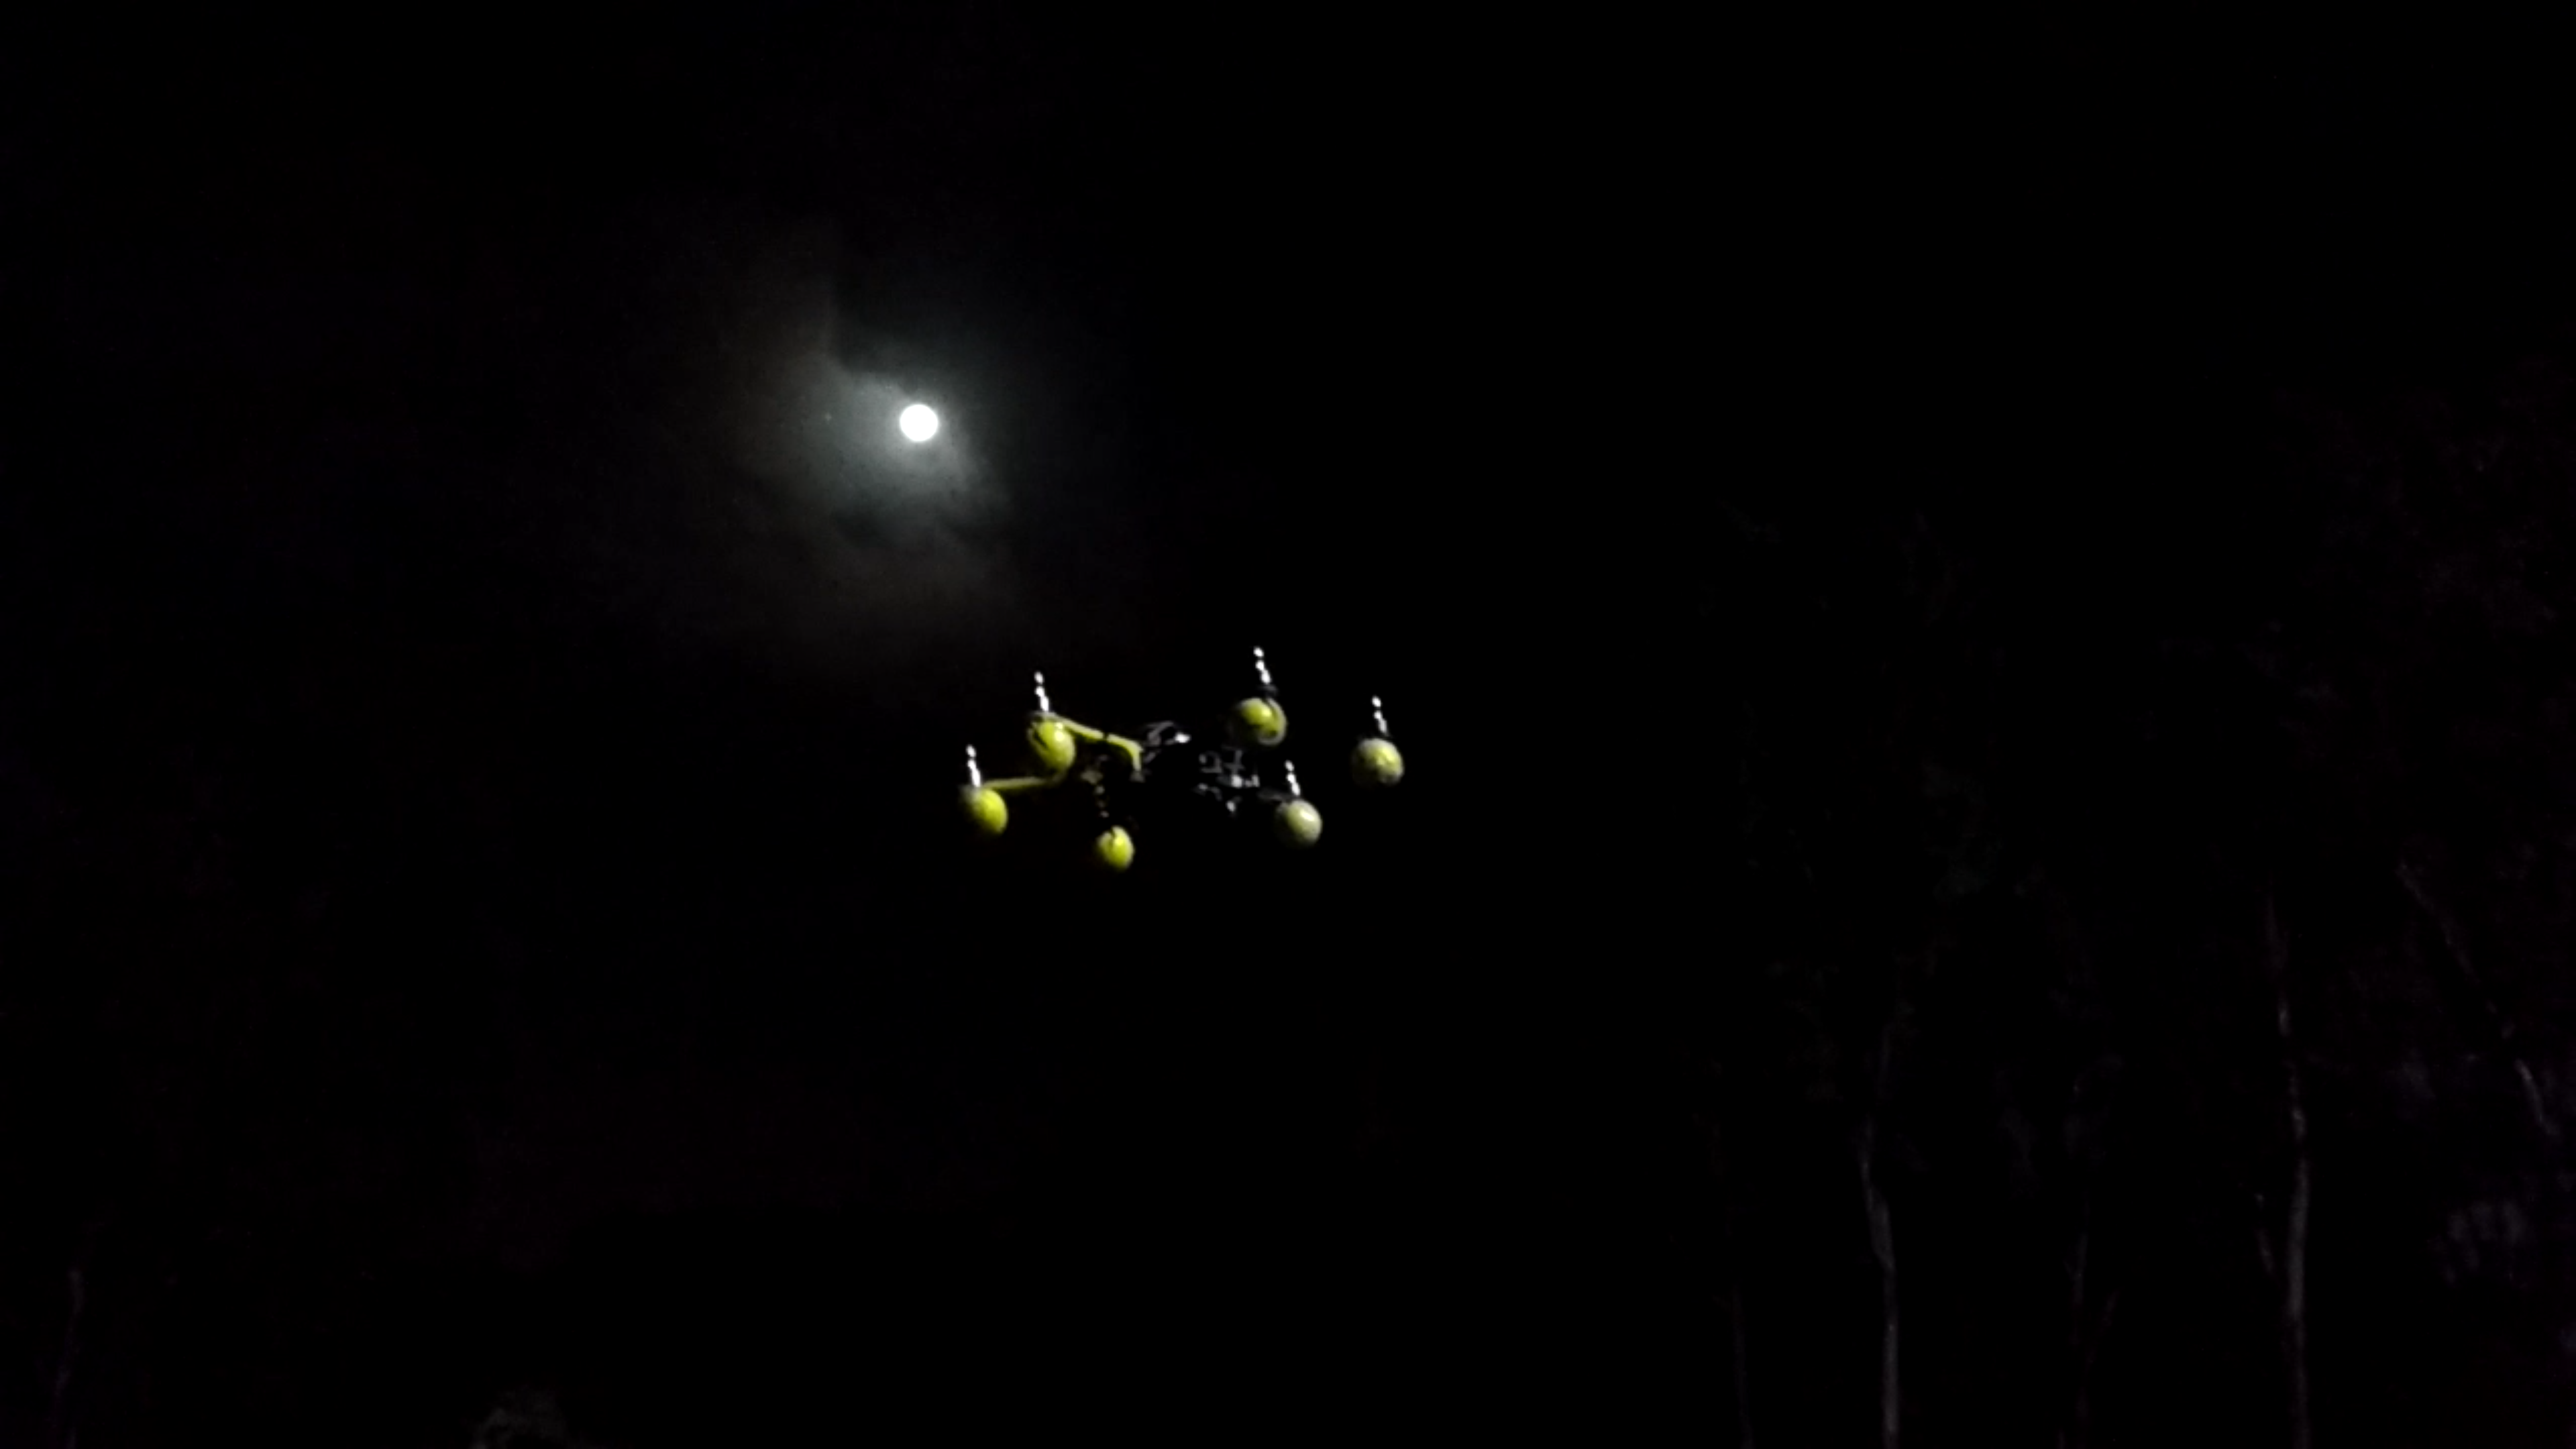
\includegraphics[width=0.48\linewidth]{auto_self_3}}
	\hfill
	\subfigure[]{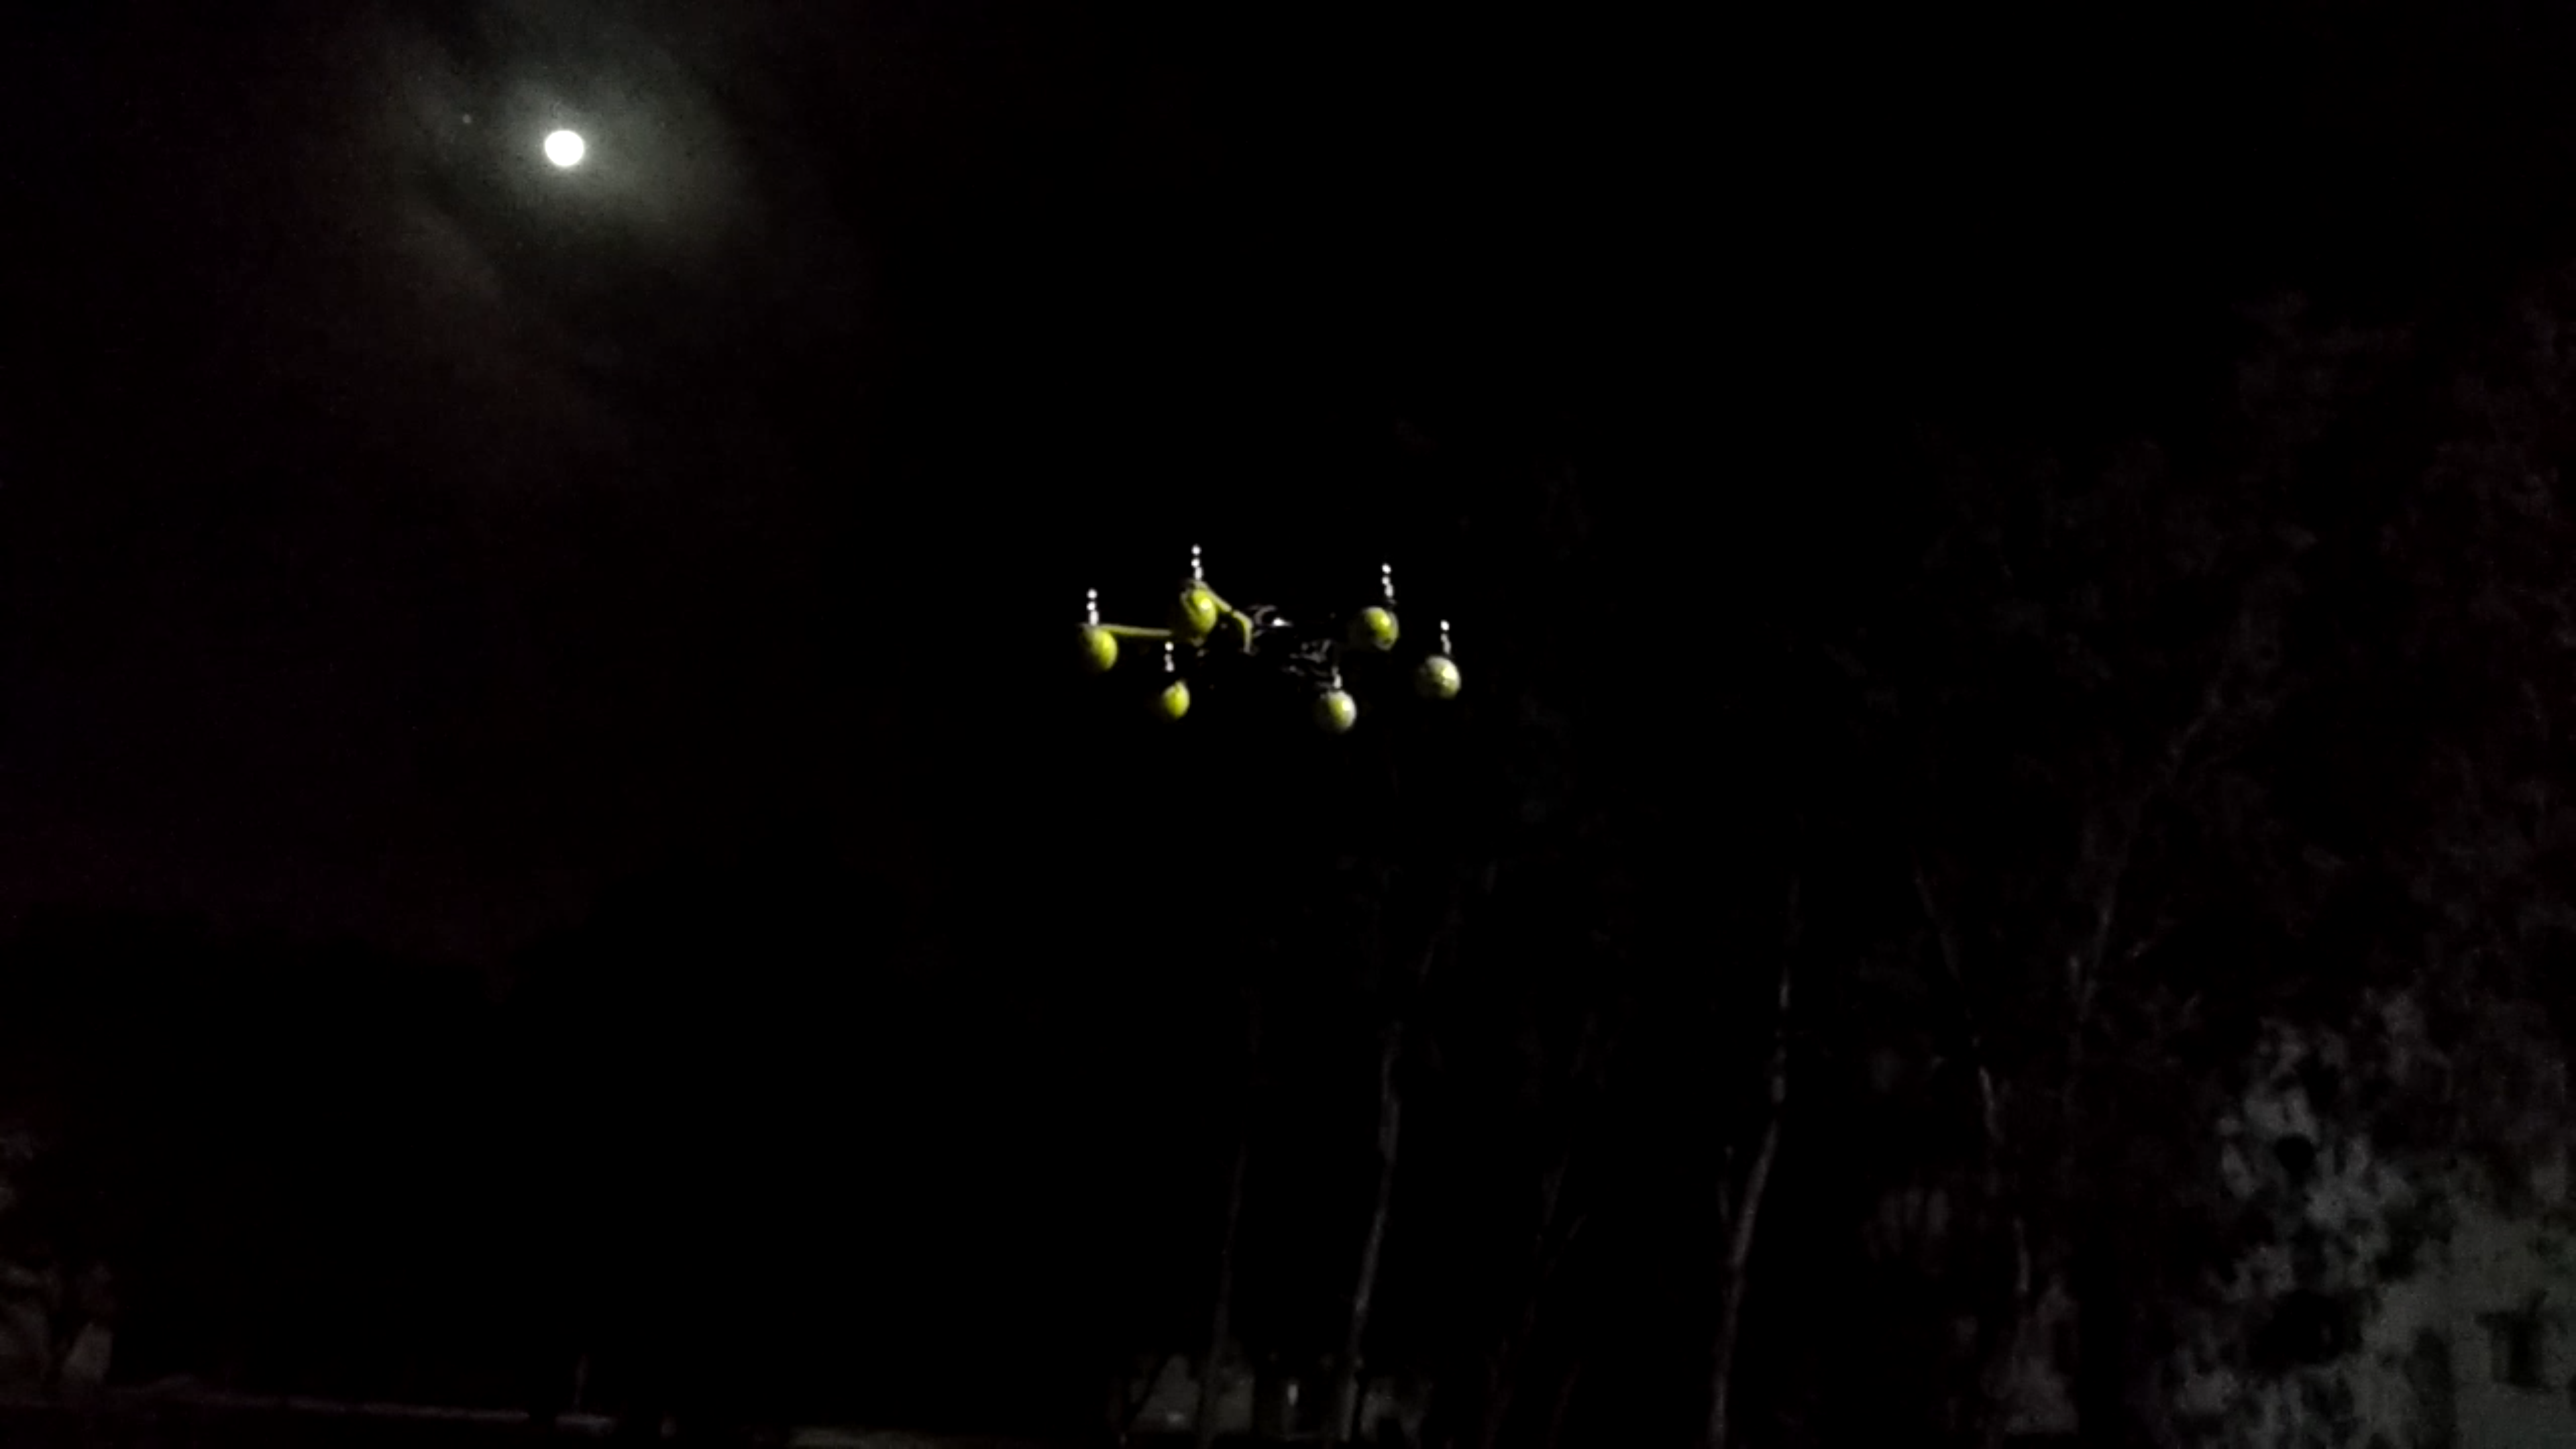
\includegraphics[width=0.48\linewidth]{auto_self_4}}
	\hfill
	\caption{\label{fig: auto_self_II}Flight test data (images) taken during night at Old CRC Lawns in SVNIT Campus}
\end{figure} 


\subsection{Planning a Mission with Waypoints and Events}

Home position, integral to our mission is needed to be set first. For that, the home position is set as the location where the copter was armed. This means if we execute an RTL in Copter, it will return to the location where it was armed, so we armed our copter in the location we wanted it to return to.
\begin{figure}[h]
	\includegraphics[width=1.0\linewidth]{svnit_auto_1}
	\centering
	\caption{\label{fig: svnit_auto_1}\textit{Arming the copter at the Old-CRC Lawns in our S.V.N.I.T. Campus}}
\end{figure}
As we can see in Fig.~\ref{fig: svnit_auto_1}, we initially armed our hex-copter near the Old-CRC lawns area in S.V.N.I.T. Campus. 

Then, as shown in Fig.~\ref{fig: svnit_auto_2}, a Copter mission starts with an auto takeoff to 5 meters attitude; then goes to WP 1, then waits 10 seconds; then the craft will proceed to WP 2 followed by WP 3, then returns to launch. After reaching the launch position, the craft will land. The mission assumes that the launch position is set at the home position.

\begin{figure}[h]
	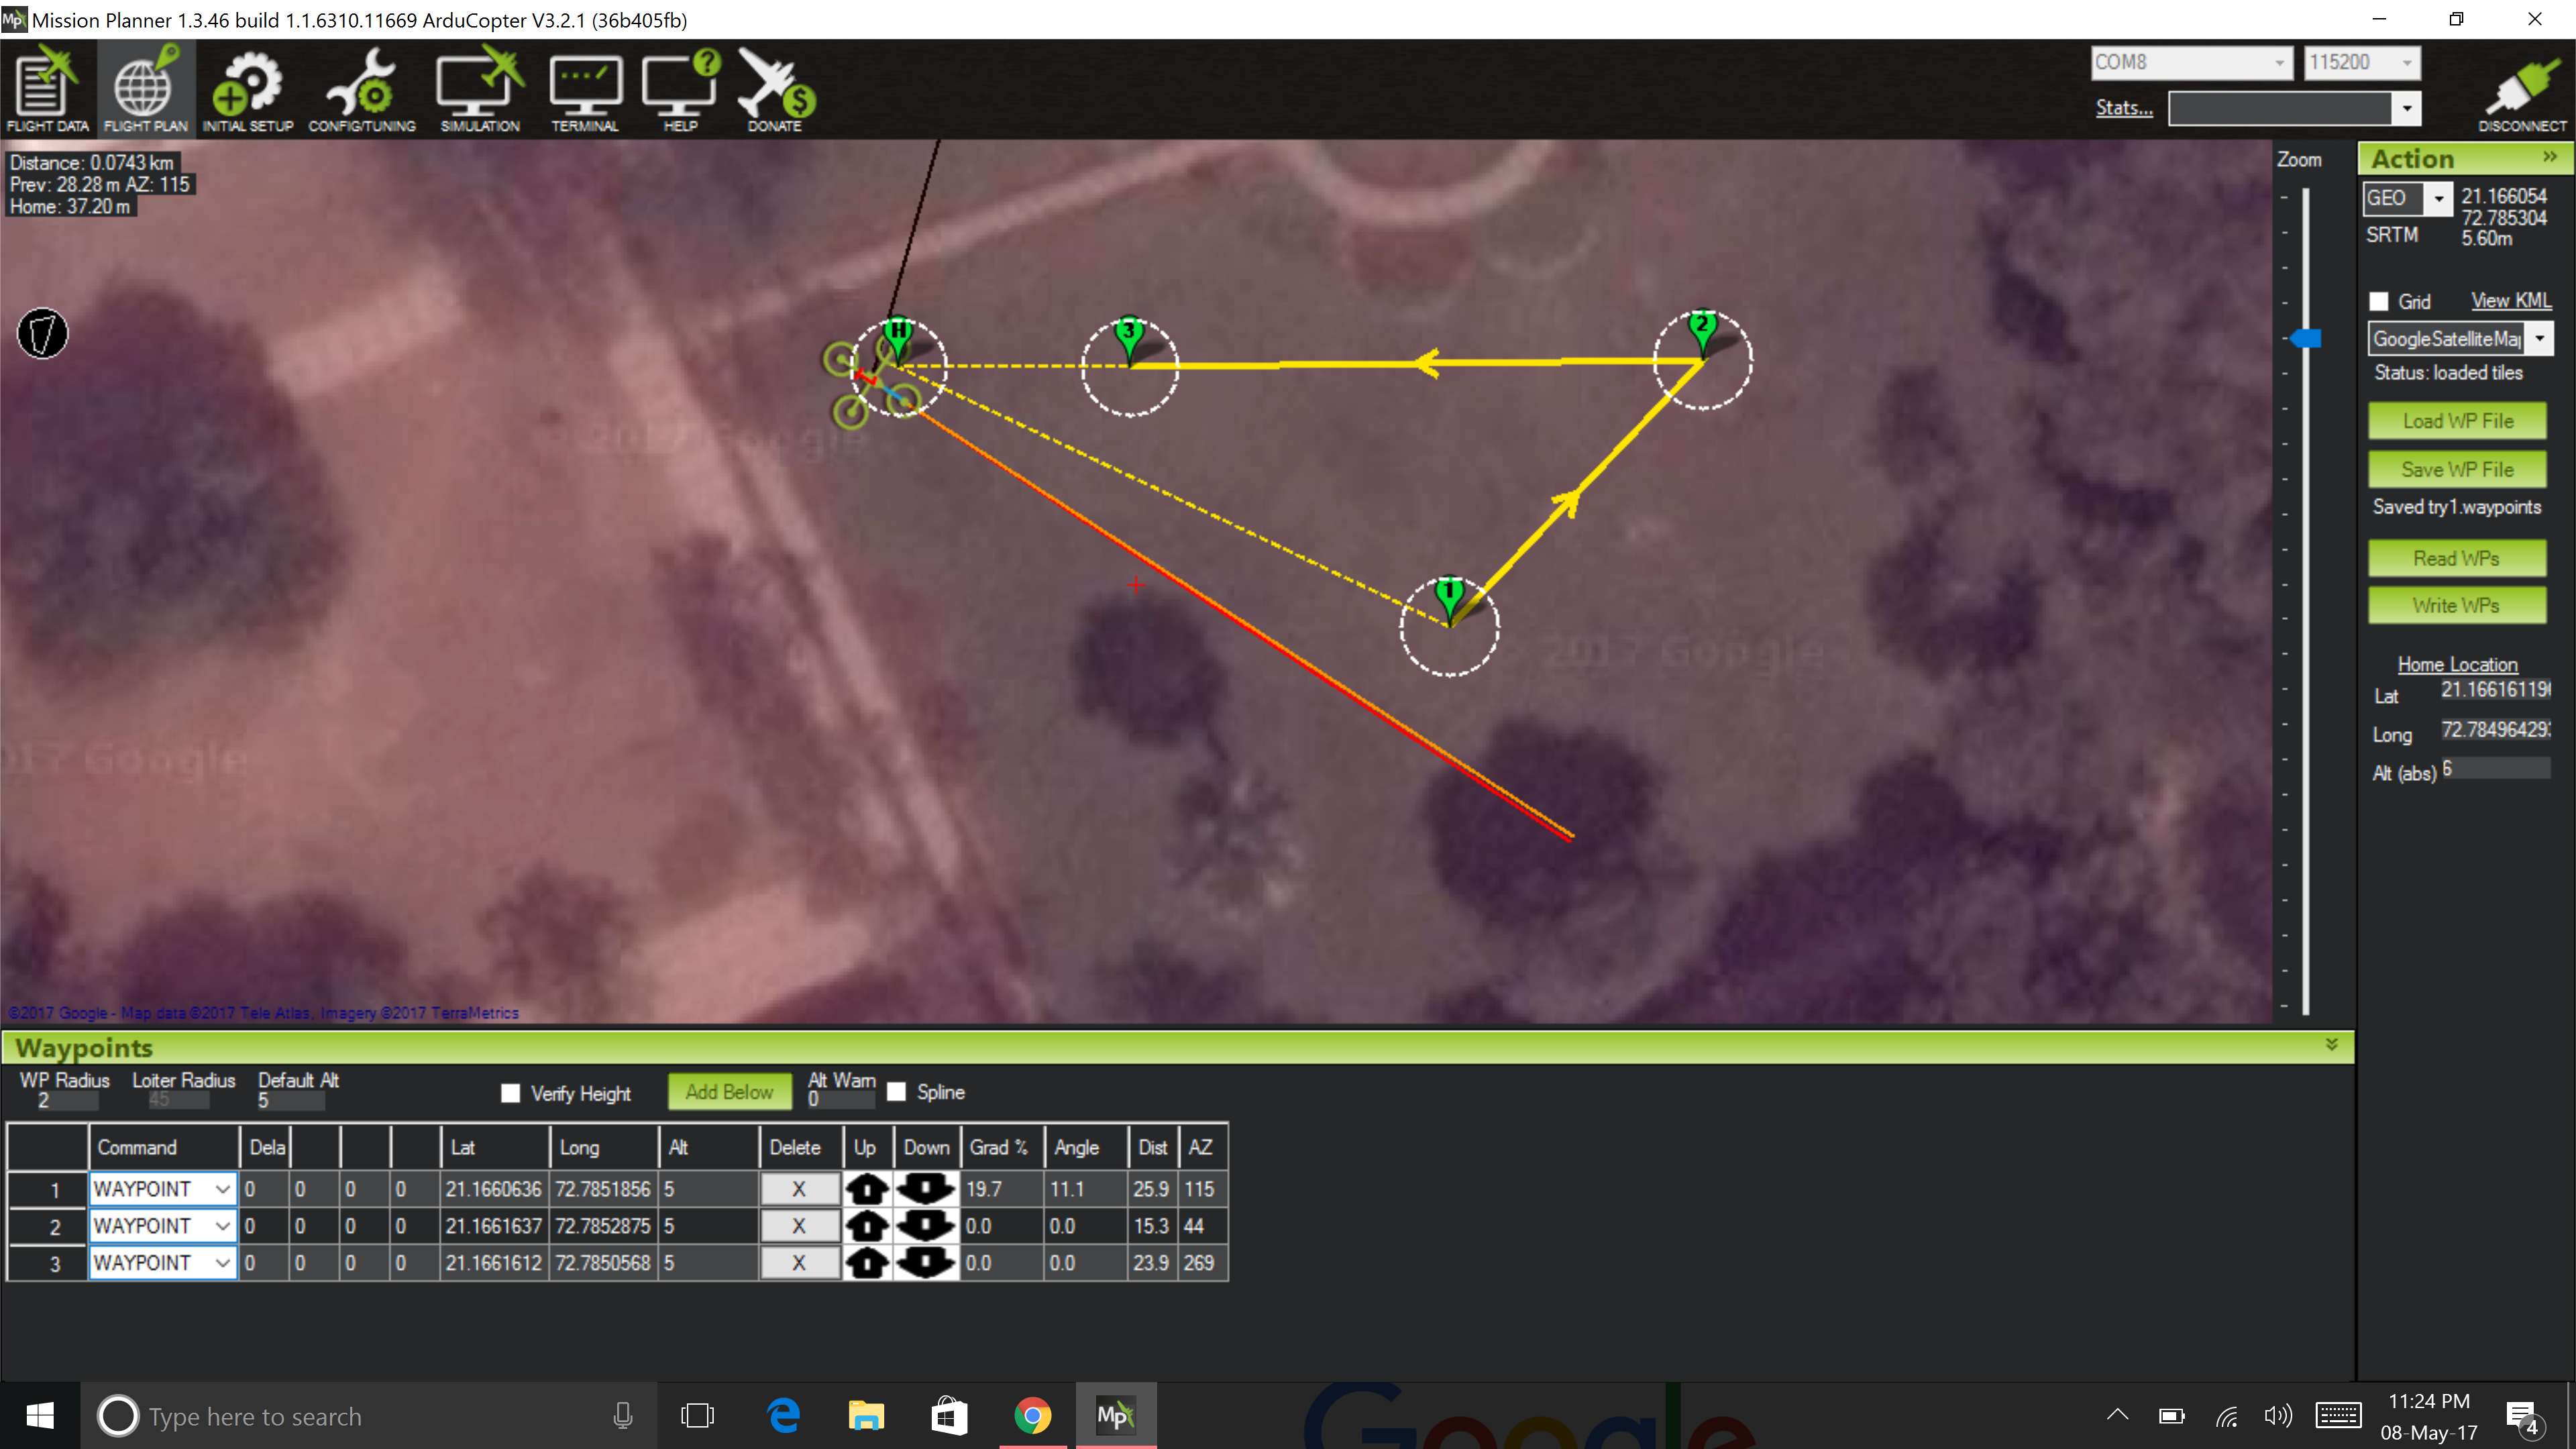
\includegraphics[width=1.0\linewidth]{svnit_auto_2}
	\centering
	\caption{\label{fig: svnit_auto_2}\textit{Planning a mission at CRC Lawns}}
\end{figure}

We can enter waypoints and other commands (see the Mission commands section below for more information). In the dropdown menus on each row, we can select the command we want. The column heading will change to show us what data that command requires. Lat and Lon can be entered by clicking on the map. Altitude is relative to our launch altitude/home position.

Once we are done with our mission, we would select Write and it will be sent to APM and saved in EEPROM. We can confirm that it’s as we wanted by selecting Read.

We can save multiple mission files to your local hard drive by selecting Save WP File or read in files with Load WP File in the right-click menu. 

\subsection{Auto grid}

To do something on the terms of precision farming needs, we know that we need our copter to fly a predetermined path obtained through GPS and survey/take available data of crops along the way. For this need, we can set such pattern in Auto grid. So we can have the Mission Planner create a mission for us, which is useful for function like mapping missions, where the aircraft should just go back and forth in a “lawnmower” pattern over an area to collect photographs (say in an agricultural field)


To do this, in the right-click menu we select Polygon and draw a box around the area you want to map. Then we select Auto WP, Grid. We then follow the dialog box process to select altitude and spacing. The Mission Planner will then generate a mission that looks something like this:
\begin{figure}[h]
	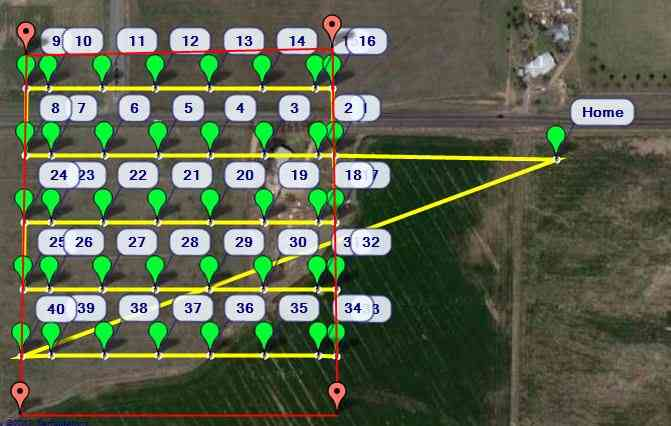
\includegraphics[width=1.0\linewidth]{mp_auto_mission_grid}
	\centering
	\caption{\label{fig: mp_auto_mission_grid}\textit{Mission pertaining to our need for precision farming application}}
\end{figure}



Below given is the detailed specification of autonomous flight accomplished in the SAC Ground, S.V.N.I.T. Campus, Surat, Gujarat, India. 

\begin{figure}[h]
	\hfill
	\subfigure[]{\includegraphics[width=0.48\linewidth]{finmis1}}
	\hfill
	\subfigure[]{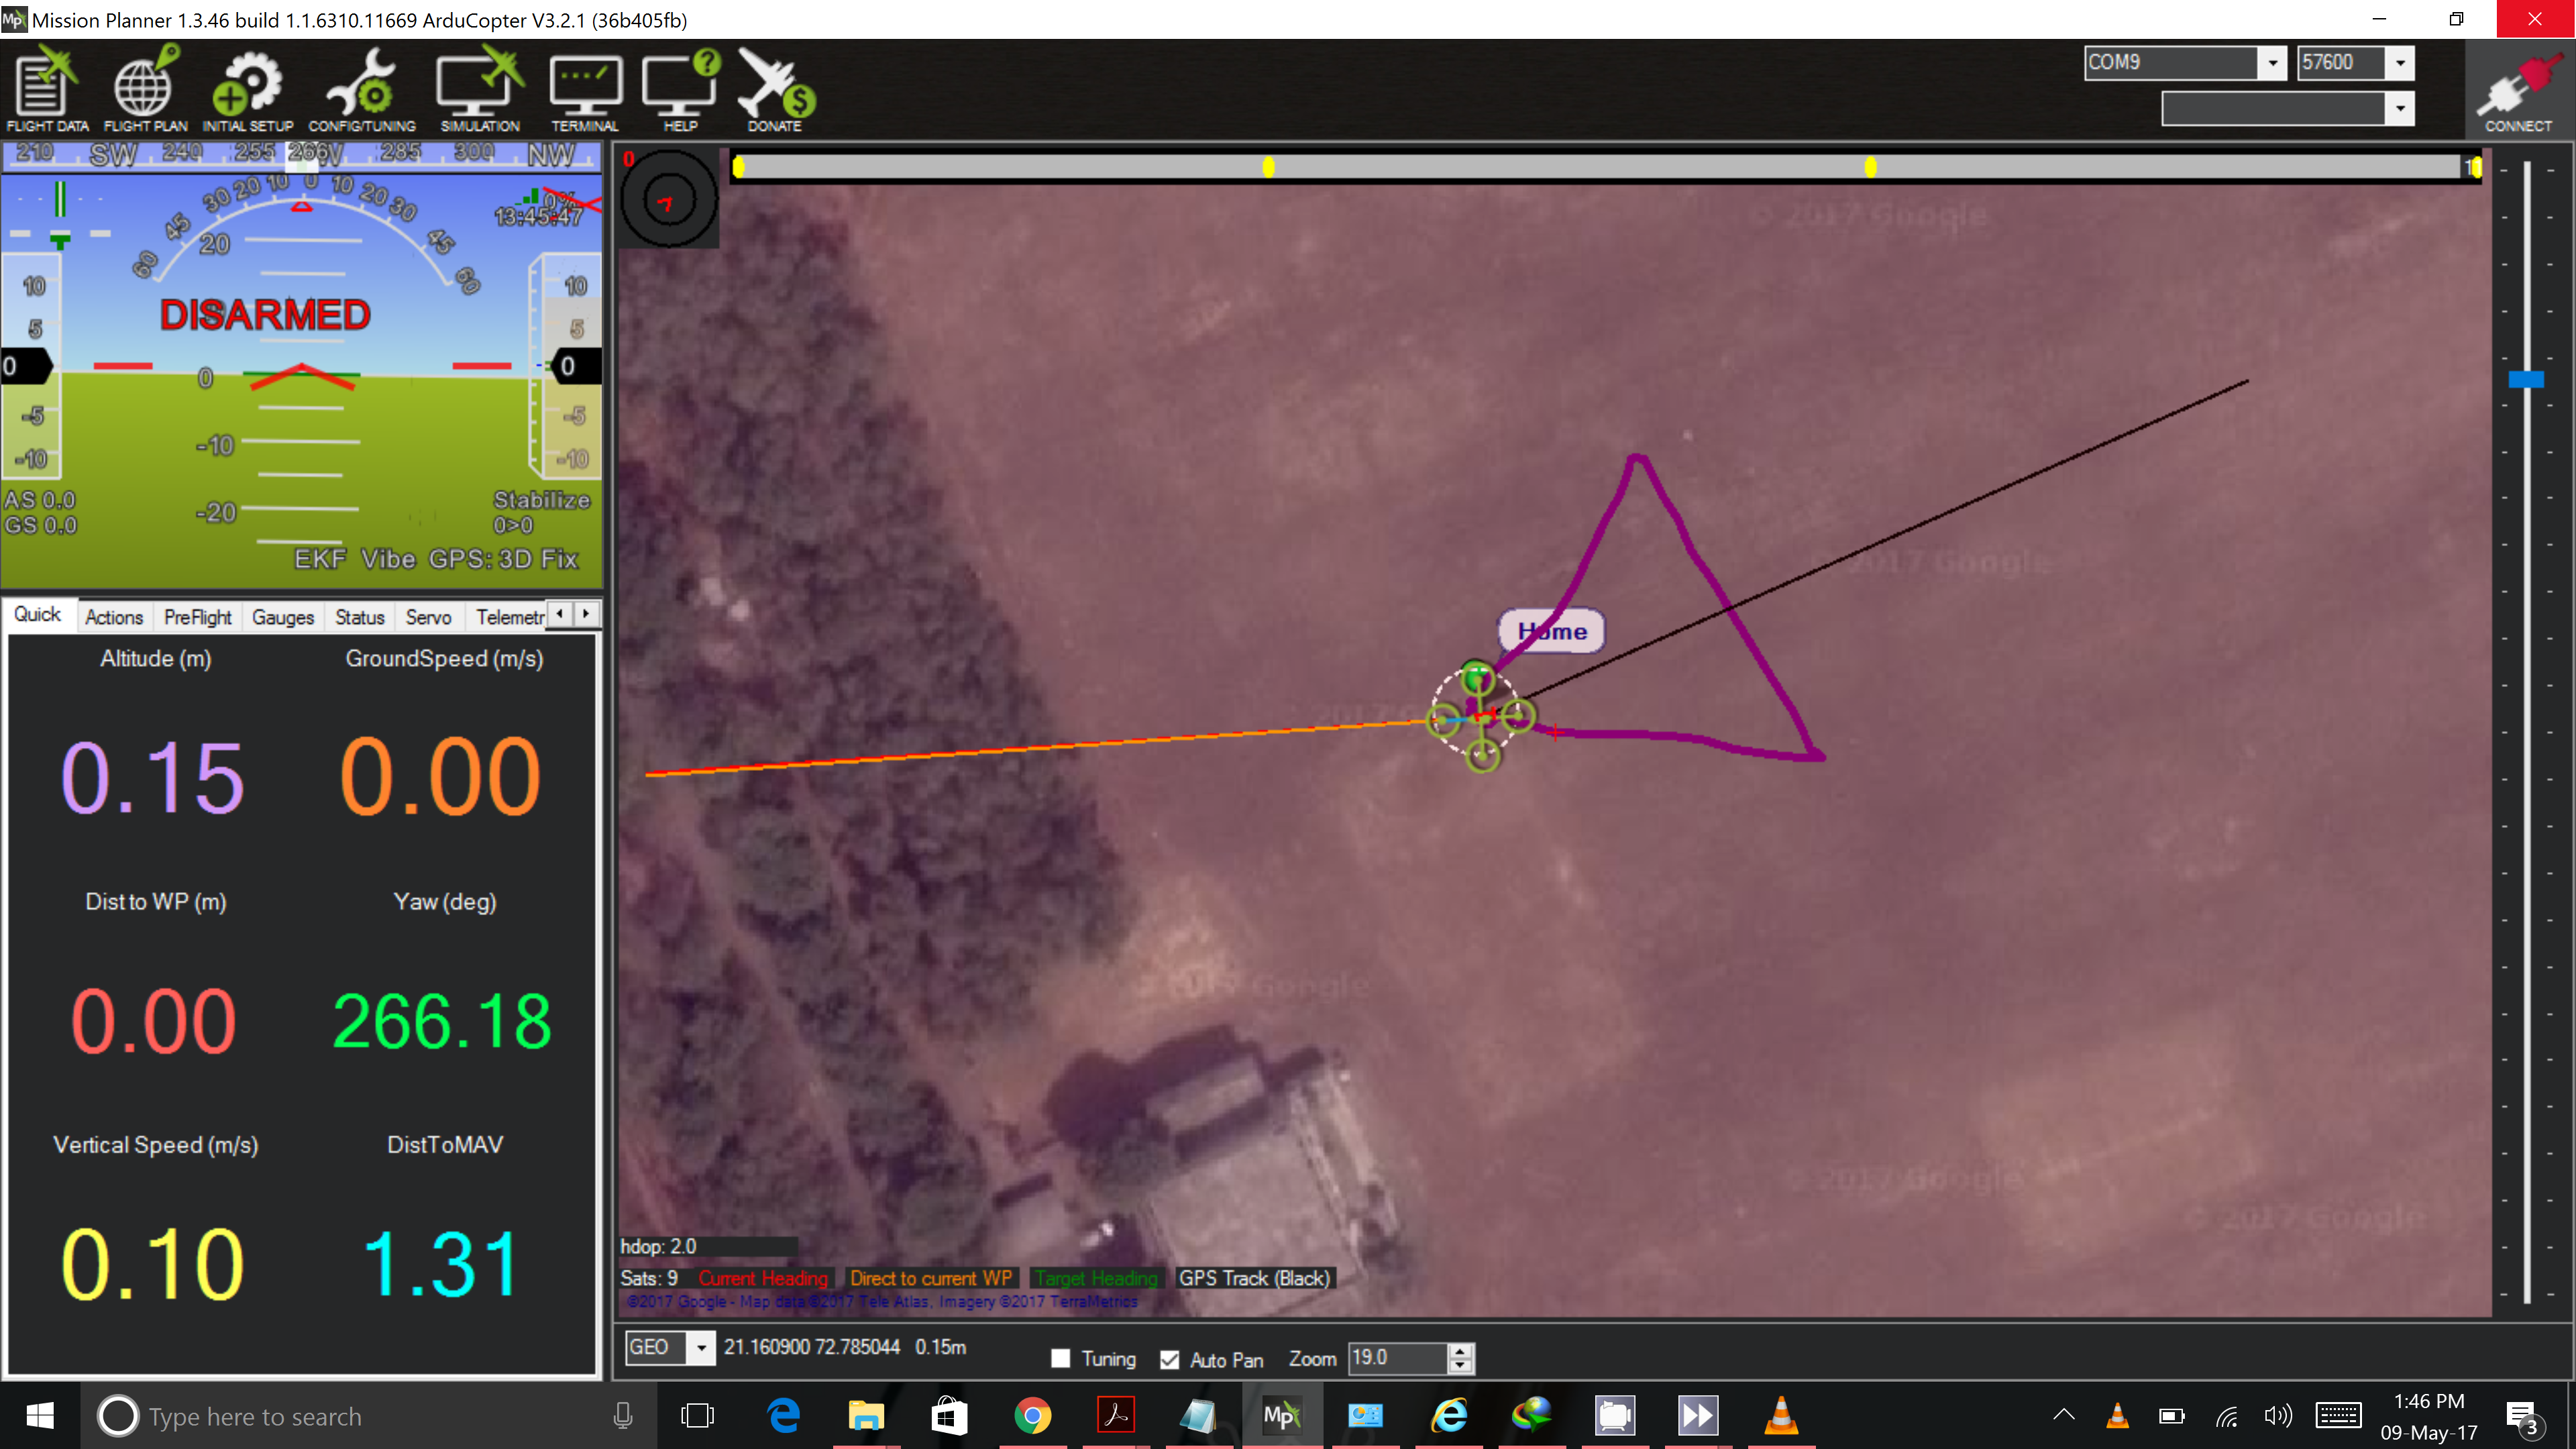
\includegraphics[width=0.48\linewidth]{finmis2}}
	\hfill
	\caption{\label{fig: fin_mis}Fig.(a) shows the desired path given by the user. Fig.(b) shows the actual traced trajectory in the autonomous mode by the hex-copter.}
\end{figure} 

Fig.~\ref{fig: fin_mis}(a) is showing the desired the path given by the GPS coordinates while Fig.~\ref{fig: fin_mis}(b) shows the actual traced trajectory by the hex-copter.

The screenshots of the autonomous flight are displayed in Fig.~\ref{fig: fin_mis_1}, Fig.~\ref{fig: fin_mis_2}, Fig.~\ref{fig: fin_mis_3} and Fig.~\ref{fig: fin_mis_4}.

\begin{figure}[!h]
	\hfill
	\subfigure[]{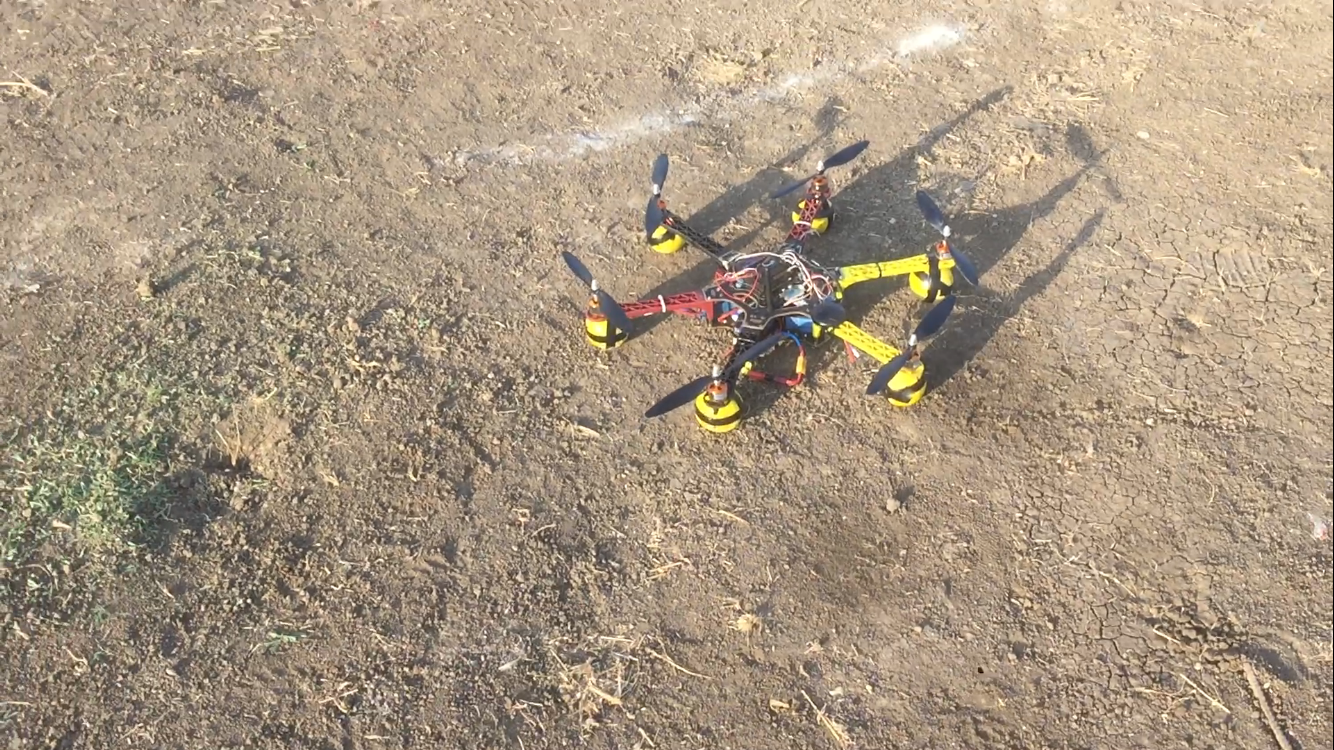
\includegraphics[width=0.48\linewidth]{finmis_1}}
	\hfill
	\subfigure[]{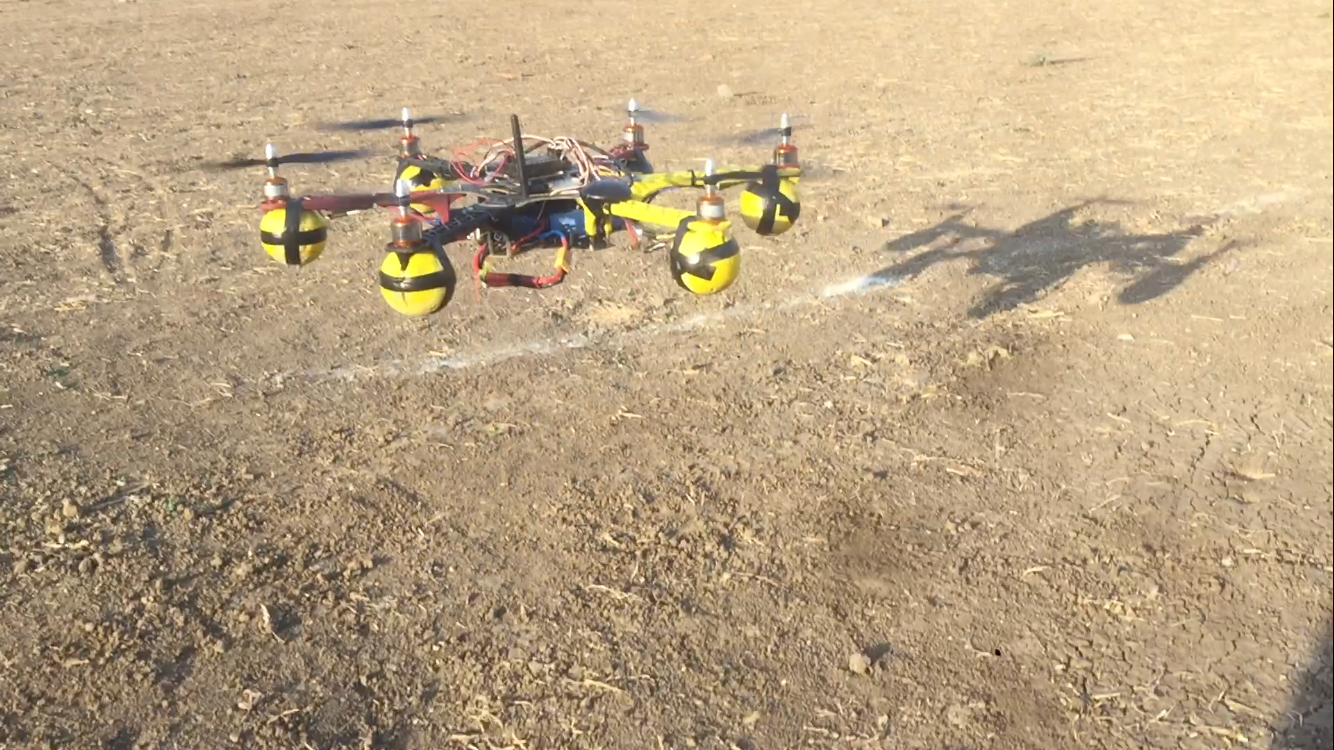
\includegraphics[width=0.48\linewidth]{finmis_2}}
	\hfill
	\caption{\label{fig: fin_mis_1}Different modes, including takeoff, hover and going to waypoints are shown above}
\end{figure} 


\begin{figure}[!h]
	\hfill
	\subfigure[]{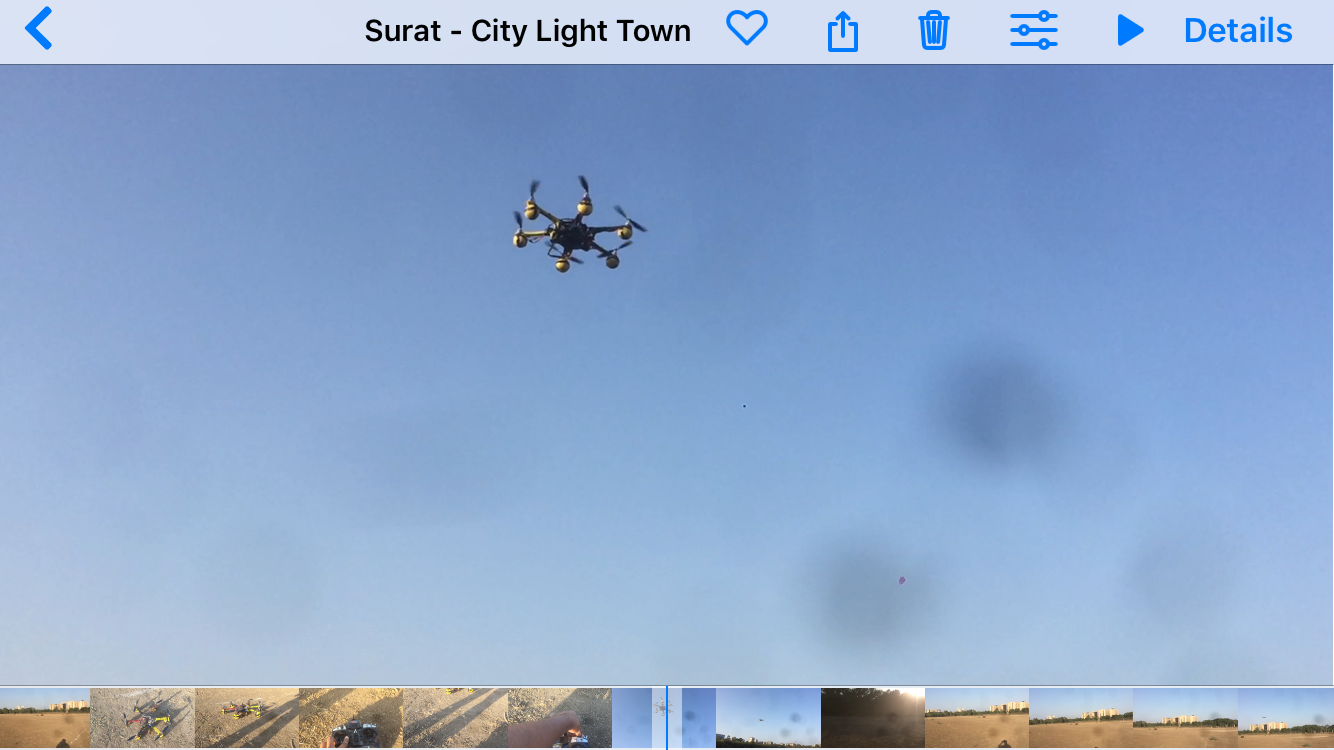
\includegraphics[width=0.48\linewidth]{finmis_3}}
	\hfill
	\subfigure[]{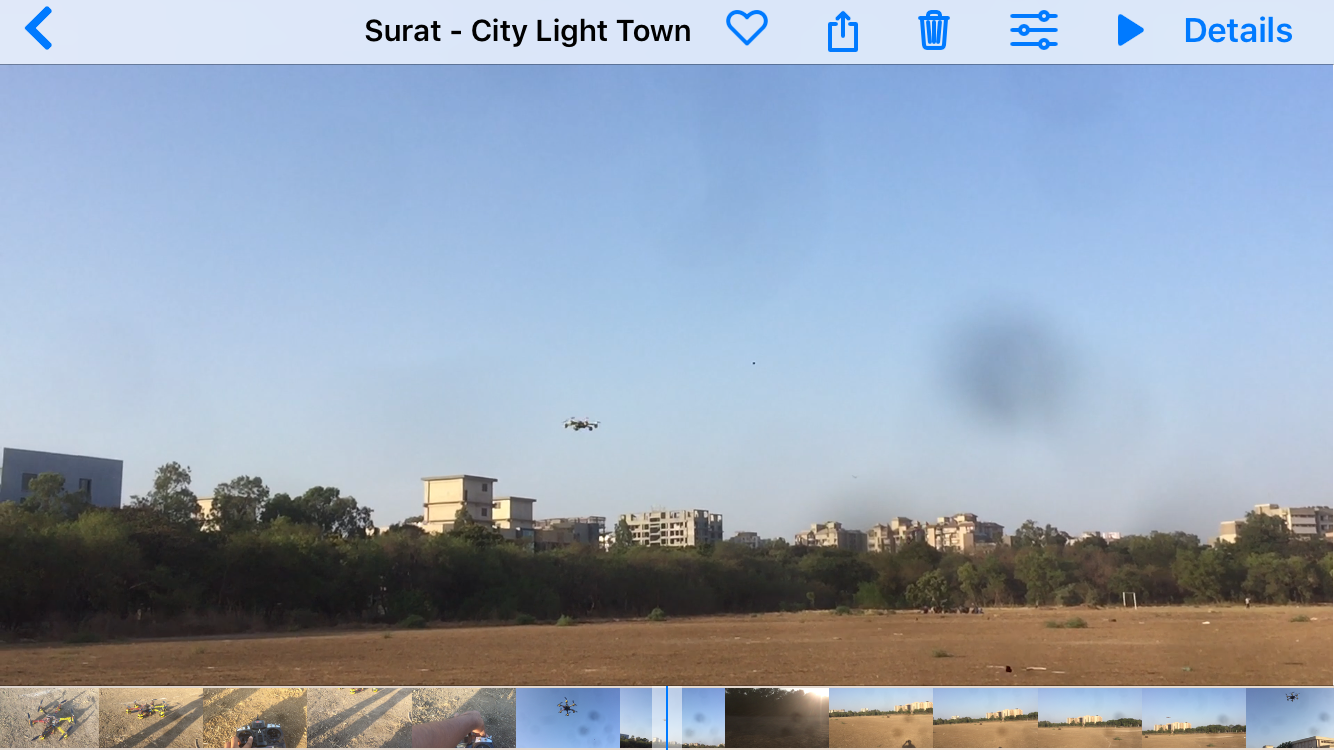
\includegraphics[width=0.48\linewidth]{finmis_4}}
	\hfill
	\caption{\label{fig: fin_mis_2}Different modes, including takeoff, hover and going to waypoints are shown above}
\end{figure} 


\begin{figure}[!h]
	\hfill
	\subfigure[]{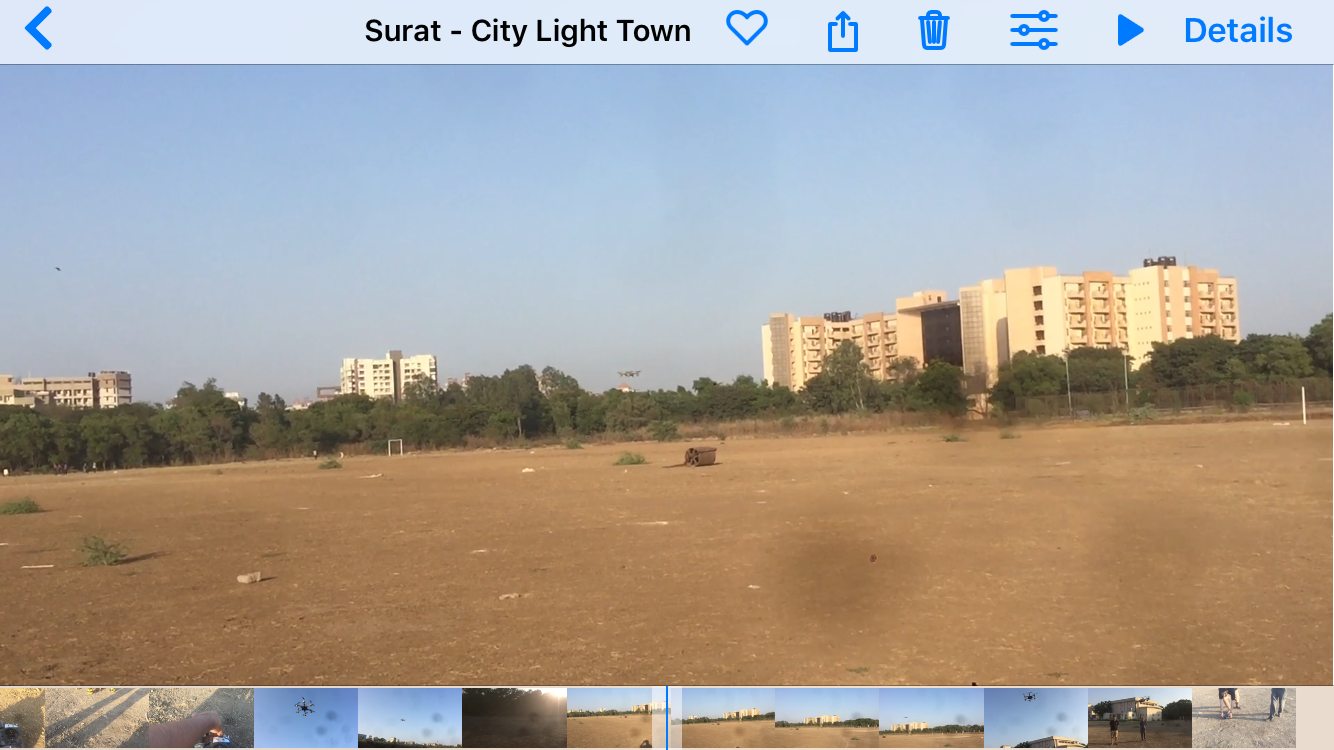
\includegraphics[width=0.48\linewidth]{finmis_5}}
	\hfill
	\subfigure[]{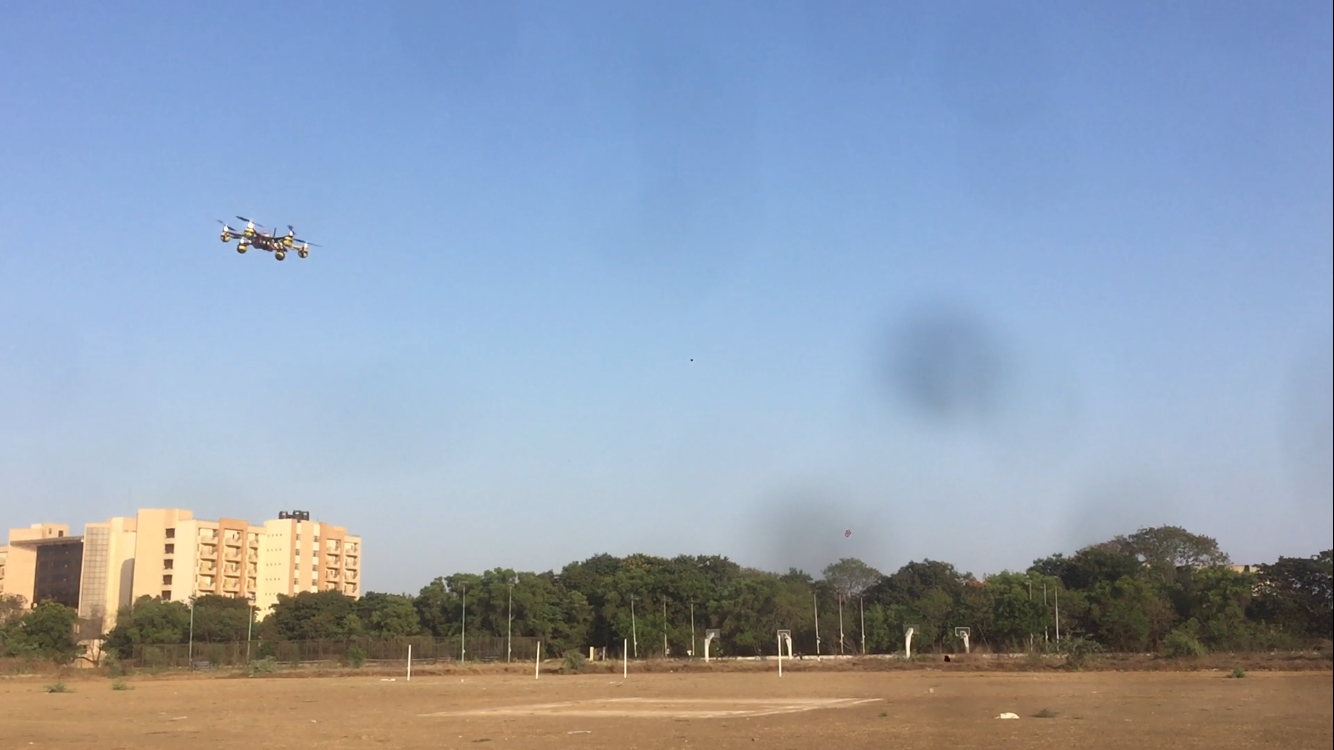
\includegraphics[width=0.48\linewidth]{finmis_6}}
	\hfill
	\caption{\label{fig: fin_mis_3}Different modes, including takeoff, hover and going to waypoints are shown above}
\end{figure} 


\begin{figure}[!h]
	\hfill
	\subfigure[]{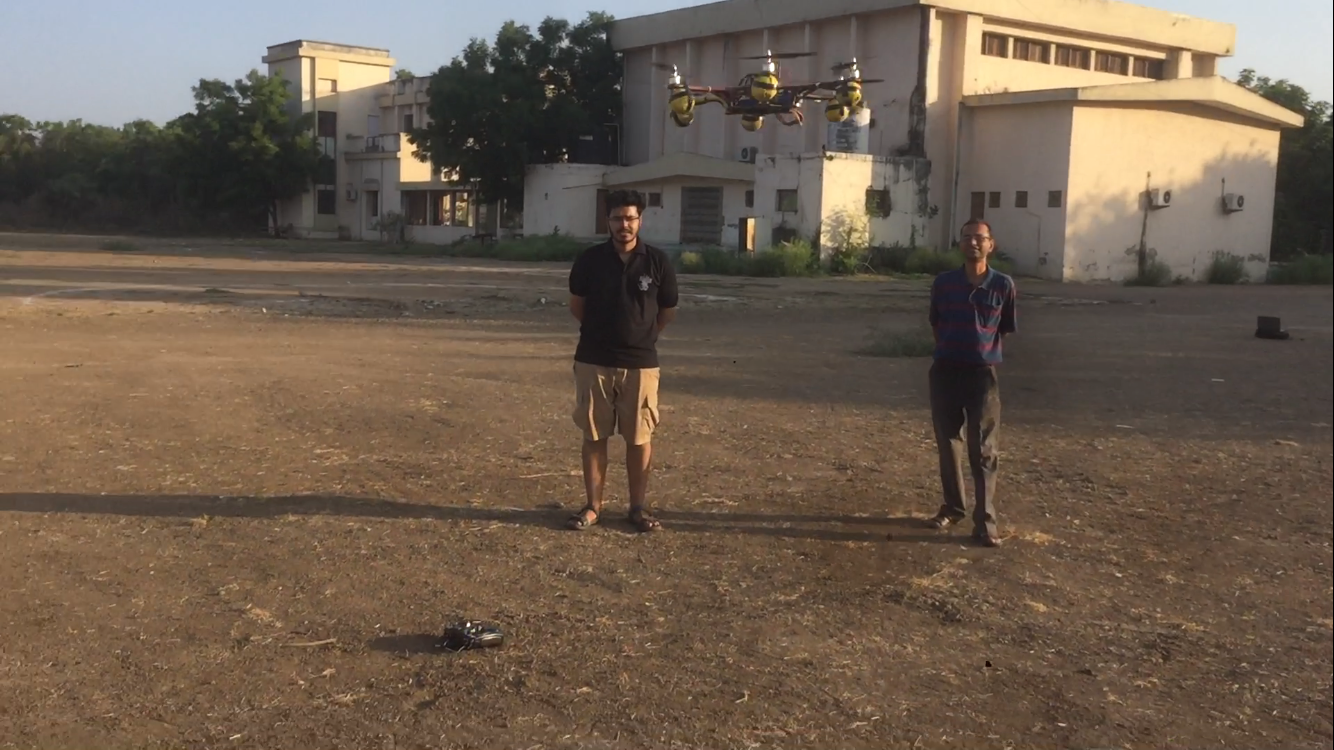
\includegraphics[width=0.48\linewidth]{finmis_7}}
	\hfill
	\subfigure[]{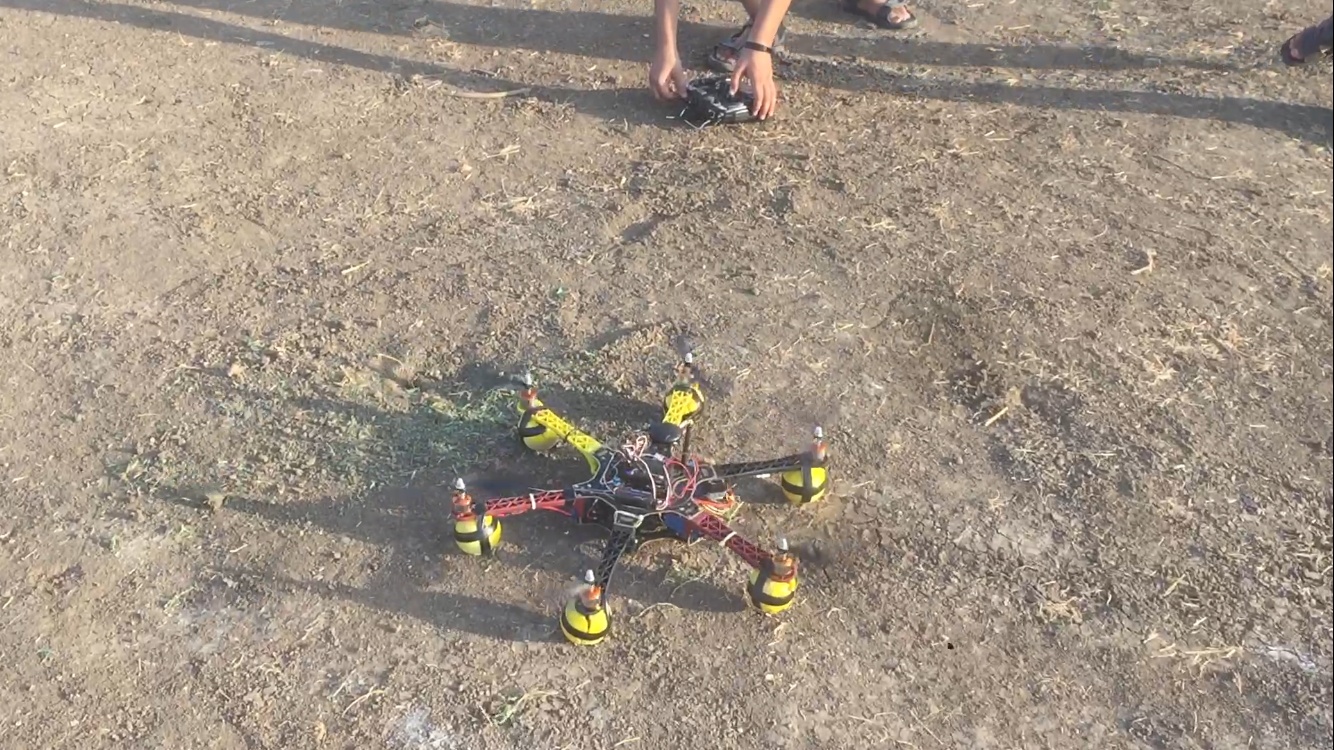
\includegraphics[width=0.48\linewidth]{finmis_8}}
	\hfill
	\caption{\label{fig: fin_mis_4}Different modes, including takeoff, hover and going to waypoints are shown above}
\end{figure} 



\section{Web Portal}

A web portal is built to facilitate the process of farm crop analysis. Web portal provides the functionality of uploading drone images for stitching process. Screenshots of the application portal are shown in Fig.~\ref{fig: web_p}, Fig.~\ref{fig: res-1} and Fig.~\ref{fig: res-2}.



\begin{figure}[h]
	\includegraphics[width=1\linewidth]{webhost_precision}
	\centering
	\caption{\label{fig: web_p}Web portal}
\end{figure}
\begin{figure}[h]
	\includegraphics[width=1\linewidth]{fin_img_15}
	\centering
	\caption{\label{fig: res-1}Image upload screen}
\end{figure}
\begin{figure}[h]
	\includegraphics[width=1\linewidth]{fin_img_16}
	\centering
	\caption{\label{fig: res-2}Dashboard for Image analysis}
\end{figure}


\subsection{Dataset for Image Stitching and NDVI Analysis}

We worked upon hyperspectral images taken from drone at Hayes Township Farm, Harrison, Michigan, USA.

Figure~\ref{fig: hyp_1}, ~\ref{fig: hyp_2} and ~\ref{fig: hyp_3} shows the hyperspectral images taken from drone. (Courtesy:6omvi.org).

Figure ~\ref{fig: hyp_4} shows the image of Hayes Township Farm, Harrison, Michigan, USA


\begin{figure}[!h]
	\hfill
	\subfigure[]{\includegraphics[width=0.48\linewidth]{fin_img_2}}
	\hfill
	\subfigure[]{\includegraphics[width=0.48\linewidth]{fin_img_3}}
	\hfill
	\caption{\label{fig: hyp_1}Hyperspectral images taken from drone (Courtesy:6omvi.org)}
\end{figure}


\begin{figure}[!h]
	\hfill
	\subfigure[]{\includegraphics[width=0.48\linewidth]{fin_img_4}}
	\hfill
	\subfigure[]{\includegraphics[width=0.48\linewidth]{fin_img_5}}
	\hfill
	\caption{\label{fig: hyp_2}Hyperspectral images taken from drone (Courtesy:6omvi.org)}
\end{figure}

\begin{figure}[!h]
	\includegraphics[width=0.5\linewidth]{fin_img_6}
	\centering
	\caption{\label{fig: hyp_3}Hyperspectral image taken from drone (Courtesy:6omvi.org)}
\end{figure}

\begin{figure}[h]
	\includegraphics[width=1.0\linewidth]{fin_img_7}
	\centering
	\caption{\label{fig: hyp_4}Hayes Township Farm,Harrison,Michigan,USA.}
\end{figure}

\subsection{Image Stitching}
Image stitching is done using OpenDroneMap (ODM) library which requires 60\% overlay between input images for accurate stitching. ODM generates a stitched image in .TIF and .PNG format which can be viewed on portal by clicking on View Image button as shown in Fig.~\ref{fig: res-3}.

\begin{figure}[h]
	\includegraphics[width=1\linewidth]{fin_img_17}
	\centering
	\caption{\label{fig: res-3}Stitched Image output}
\end{figure}

\subsection{NDVI Analysis}

In our application we calculated NDVI using QGIS (Quantum GIS) python programing language APIs. We use QgsRasterLayer class that provides QGIS with the ability to render raster (image) datasets onto the map canvas. From loaded raster we are extracting IR and Red bands for NDVI calculation. QgsRasterCalculator (expression, output file, ``GTiff'', extent, width, height, entries) class generates NDVI image with the help of QgsRasterCalculator .processCalculation () method. View NDVI button calculates the NDVI of the stitched image as shown in Fig.~\ref{fig: stitching}

\begin{figure}[h]
	\hfill
	\subfigure[]{\includegraphics[width=0.48\linewidth]{fin_img_9}}
	\hfill
	\subfigure[]{\includegraphics[width=0.48\linewidth]{fin_img_10}}
	\hfill
	\caption{\label{fig: stitching}\textbf{(a)} Input stitched image \& \textbf{(b)} NDVI output Image}
\end{figure}

\subsection{Clustering using K-Means}

We clustered the data into k = 4 classes depending upon the range of NDVI values as given by . This clustered data is used to train the SoftMax regression model.


\subsection{SoftMax Regression Model}

We built a softmax regression model using Google’s tensorflow and trained it upon the clustered dataset generated from above step. With 80\% training and 20\% test data we achieved an accuracy of about 70\%. This can be improved once we have better labelled dataset. The layered structure of the built model as visualized in TensorBoard is shown in Fig.~\ref{fig: softmax regression}

\begin{figure}[t]
	\includegraphics[width=1.0\linewidth]{fin_img_12}
	\centering
	\caption{\label{fig: softmax regression}Softmax Regression Model(Visualized in Tensorboard)}
\end{figure}

\textbf{Analysis 1 Tab}: Clicking on this button evaluates the newly created NDVI image via the Softmax Model to divide the input image into different colour coded regions as shown in Fig.~\ref{fig: res-4}

\begin{figure}[h]
	\hfill
	\subfigure[]{\includegraphics[width=0.48\linewidth]{fin_img_18}}
	\hfill
	\subfigure[]{\includegraphics[width=0.48\linewidth]{fin_img_19}}
	\hfill
	\caption{\label{fig: res-4}\textbf{(a)} Stitched image \& \textbf{(b)} Colour coded regions}
\end{figure}


Finally the image of the farm is overlaid over the Google Maps as shown in Fig.~\ref{fig: res-5}

\begin{figure}[h]
	\includegraphics[width=1\linewidth]{fin_img_20}
	\centering
	\caption{\label{fig: res-5}NDVI analysed image overlaid on Google Map}
\end{figure}



\subsection{Dataset for Deep Learning}

We used a public dataset~\cite{PlantVil94:online} of 54,306 images of diseased and healthy plant leaves collected under controlled conditions to identify 14 crop species and 26 diseases (or absence thereof).An example of leaf images form the PlantVillage dataset, representing 38 crop-disease pair is hsown in Fig.~\ref{fig: dataset_image}.

\begin{figure}[!h]
	\includegraphics[width=1\linewidth]{fin_img_1}
	\centering
	\caption{\label{fig: dataset_image}Example of leaf images from the PlantVillage dataset, representing every crop-disease pair used \textbf{(1)} Apple Scab, \textit{Venturia inaequalis} \textbf{(2)} Apple Black Rot, \textit{Botryosphaeria obtusa} \textbf{(3)} Apple Cedar Rust,  \textit{Gymnosporangium juniperi-virginianae} \textbf{(4)} Apple healthy \textbf{(5)} Blueberry healthy \textbf{(6)} Cherry healthy \textbf{(7)} Cherry Powdery Mildew, \textit{Podoshaera clandestine} \textbf{(8)} Corn Gray Leaf Spot, \textit{Cercospora zeae-maydis} \textbf{(9)} Corn Common Rust, \textit{Puccinia sorghi} \textbf{(10)} Corn healthy \textbf{(11)} Corn Northern Leaf Blight, \textit{Exserohilum turcicum} \textbf{(12)} Grape Black Rot, \textit{Guignardia bidwellii}, \textbf{(13)} Grape Black Measles (Esca), \textit{Phaeomoniella aleophilum, Phaeomoniella chlamydospora} \textbf{(14)} Grape Healthy \textbf{(15)} Grape Leaf Blight, \textit{Pseudocercospora vitis} \textbf{(16)} Orange Huanglongbing (Citrus Greening), \textit{Candidatus Liberibacter spp.} \textbf{(17)} Peach Bacterial Spot, \textit{Xanthomonas campestris} \textbf{(18)} Peach healthy \textbf{(19)} Bell Pepper Bacterial Spot, \textit{Xanthomonas campestris} \textbf{(20)} Bell Pepper healthy \textbf{(21)} Potato Early Blight, \textit{Alternaria solani} \textbf{(22)} Potato healthy \textbf{(23)} Potato Late Blight, \textit{Phytophthora infestans} \textbf{(24)} Raspberry healthy \textbf{(25)} Soybean healthy \textbf{(26)} Squash Powdery Mildew, \textit{Erysiphe cichoracearum} \textbf{(27)} Strawberry Healthy \textbf{(28)} Strawberry Leaf Scorch, \textit{Diplocarpon earlianum} \textbf{(29)} Tomato Bacterial Spot, \textit{Xanthomonas campestris pv. vesicatoria} \textbf{(30)} Tomato Early Blight, \textit{Alternaria solani} \textbf{(31)} Tomato Late Blight, \textit{Phytophthora infestans} \textbf{(32)} Tomato Leaf Mold, \textit{Passalora fulva} \textbf{(33)} Tomato Septoria Leaf Spot, \textit{Septoria lycopersici} \textbf{(34)} Tomato Two Spotted Spider Mite, \textit{Tetranychus urticae} \textbf{(35)} Tomato Target Spot, \textit{Corynespora cassiicola} \textbf{(36)} Tomato Mosaic Virus \textbf{(37)} Tomato Yellow Leaf Curl Virus \textbf{(38)} Tomato healthy.}
\end{figure}


\subsection{Crop Disease Prediction Using Deep Learning}

Using the deep convolutional neural network architecture, we trained the inception V-3 model on images of plant leaves with the goal of classifying both crop species and the presence and identity of disease on images that the model had not seen before. The images were resized to 256x256 pixels as required by the inception model. Within the PlantVillage data set of 54,306 images containing 38 classes of 14 crop species and 26 diseases (or absence thereof), and with 70\% training while 30\% validation datasets this goal has been achieved as demonstrated by the top accuracy of 99\% upon training till 3900 steps for 23 hours on 32GB RAM CPU with 8GB of NVIDIA GeForce 980M GTX graphics card. Thus, without any feature engineering, the model correctly classifies crop and disease from 38 possible classes in 990 out of 1000 images. Importantly, while the training of the model takes a lot of time (multiple hours on a high performance GPU cluster computer), the classification itself is very fast (less than a second on a CPU), and can thus easily be implemented on a smartphone.


\subsubsection{Limitations}
However, this approach helps the farmers to get prescription of the crop problems, there are certain limitations to it. In this experiment we are currently constrained to  the classification of single leaves, facing up, on a homogeneous background. While these are straightforward conditions, a real world application should be able to classify images of a disease as it presents itself directly on the plant. Indeed, many diseases don’t present themselves on the upper side of leaves  only (or at all), but on many different parts of the plant. Thus, new image collection efforts should try to obtain images from many different perspectives, and ideally from settings that are as realistic as possible. This way we can get better accuracies in practical problems.

\textbf{Analysis Tab 2}: Clicking on this button on the portal asks the user to upload an image of the crops (taken by smartphone) which is evaluated against the trained inception v-3 model.


Example input image as shown in Fig.~\ref{fig: res-6} gives the output:

\begin{figure}[!h]
	\includegraphics[width=0.5\linewidth]{fin_img_21}
	\centering
	\caption{\label{fig: res-6}Input image of crop}
\end{figure}

\textbf{Class 12: Grape Black Rot, \textit{Guignardia bidwellii} (crop-disease pair)}.

\textbf{Cause:} “Grape black rot is a fungal disease caused by an ascomycetous fungus, \textit{Guignardia bidwellii}, that attacks grape vines during hot and humid weather”

\textbf{Control:} A mixture of cultural and chemical control practices can manage grape black rot disease caused by Guignardia bidwellii. Cultural control aspects involve the basics in plant care and field sanitation as well as clean-up after an infectious outbreak. Chemical control has a large influence to eliminate disease.

A similar workflow in Android Application is shown in Fig.~\ref{fig: scr1andscr2} and Fig.~\ref{fig: scr3andscr4}.

\begin{figure}[!h]
	\hfill
	\subfigure[]{\includegraphics[height=0.48\linewidth]{scr-4}}
	\hfill
	\subfigure[]{\includegraphics[height=0.48\linewidth]{scr-3}}
	\hfill
	\caption{\label{fig: scr3andscr4}Fig.~\ref{fig: scr3andscr4}(a) describes Home Screen of Android Application. Fig.~\ref{fig: scr3andscr4}(b) shows Stitched image output}
\end{figure}


\begin{figure}[!h]
	\hfill
	\subfigure[]{\includegraphics[height=0.48\linewidth]{scr-2}}
	\hfill
	\subfigure[]{\includegraphics[height=0.48\linewidth]{scr-1}}
	\hfill
	\caption{\label{fig: scr1andscr2}Fig.~\ref{fig: scr1andscr2}(a) describes overlay of stitched image on Google Maps. Fig.~\ref{fig: scr1andscr2} describes prescription of crops in critical areas of the farm.}
\end{figure} % Experimental Results
	
	\chapter{Conclusions and Future Work}

We have successfully made an open-source end-user system which provides the farmer with all the functionalities to analyse and improve the farm health. The drone is made autonomous for surveying/scanning the farm. Image stitching is then done using OpenDroneMap library. Application of NDVI combined with SoftMax regression model gave us an accuracy of about 70\% in detecting critical areas on the farm. Analysis of the images taken by the smartphone of the critical areas on the farm is also done using Google’s Inception V-3 model receiving an accuracy of about 99\%. An easy to use web and android based application is also made to ease user’s access. Thus a low cost system for precision farming has been built using all open-source software and libraries with minimal proprietary cost. Since, we have made our own labelled dataset using clustering and trained our machine learning model on this data this creates inaccuracy in results which can be improved once we have a better labelled dataset. We can also make use of more VI methods like Soil Adjusted Vegetation Index (SAVI), Enhanced NDVI (ENDVI), etc. to improve the accuracy of our machine learning model. Also the limitations in the deep learning model can be removed once we have an improved dataset which includes pictures taken from various angles, having varied backgrounds, etc. so that the model becomes more feasible for practical scenarios. The application just now runs on localhost and needs to be deployed on a server.   % Conclusions and Future Work	
	
	%% ----------------------------------------------------------------
	% Now begin the Appendices, including them as separate files
	
	\addtocontents{toc}{\vspace{2em}} % Add a gap in the Contents, for aesthetics
	
	%\appendix % Cue to tell LaTeX that the following 'chapters' are Appendices
	
	%\chapter{An Appendix}

Add appendices here	% Appendix Title
	
	%\input{Appendices/AppendixB} % Appendix Title
	
	%\input{Appendices/AppendixC} % Appendix Title
	
	\addtocontents{toc}{\vspace{2em}}  % Add a gap in the Contents, for aesthetics
	\backmatter
	
	%% ----------------------------------------------------------------
	\label{Bibliography}
	\lhead{\emph{Bibliography}}  % Change the left side page header to "Bibliography"
	\bibliographystyle{IEEEtran}  % Use the "unsrtnat" BibTeX style for formatting the Bibliography
	%\bibliographystyle{../support/IEEEtran}
	\bibliography{Bibliography}  % The references (bibliography) information are stored in the file named "Bibliography.bib"
	
\end{document}  % The End
%% ----------------------------------------------------------------